\documentclass[a4paper,12pt,british]{memoir}
\usepackage[utf8]{inputenc}
\usepackage{babel}
\isopage
\checkandfixthelayout
\pagestyle{ruled}
%\raggedbottom
\usepackage[noamssymb,noamsthm,envcountsect]{beamerarticle}
\setjobnamebeamerversion{main.presentation}

\setfloatlocations{figure}{hbtp}
\setfloatlocations{table}{htbp}

% Lists
\usepackage{multicol}
\usepackage[inline]{enumitem}
\newlist{inlinelist}{enumerate*}{1}
\setlist[inlinelist]{label=(\roman*)}
\firmlists
\renewcommand*{\descriptionlabel}[1]{\hspace\labelsep\itshape #1 --}

% Epigraphcs and quotes
\setlength{\epigraphwidth}{.6\textwidth}

% Extra and background information boxes
\usepackage[most]{tcolorbox}
\usepackage{fontawesome}
%\usepackage{manfnt}
%\usepackage{lettrine}
%\newenvironment{extrainfo}{%
%  \color{red}\lettrine[lines=2]{\faFloppyO}{a}%
%}{}
\newtcolorbox{extrainfo}{
   title = {\faUniversity\quad Extra information},
   colframe = BorderColourExtraInfo,
   colback = white,
   breakable = true
}
%\newtcolorbox{backgroundinfo}{
%   title = {\faFloppyO\quad Background information},
%   colframe = BorderColourBackgroundInfo,
%   colback = white
%   }
  
% Figures and tables
\usepackage{caption}
\captionsetup{
    font={small,sf},
    labelfont={sc,color=labelcolor},
    labelsep=endash
    }
\captionsetup[table]{position=above}
\captionsetup[figure]{position=below}
\usepackage{subcaption}
\usepackage{graphicx}
\setkeys{Gin}{width=.75\textwidth} % from the graphicx package

\usepackage{csquotes}
\usepackage[backend=biber,style=reading,citestyle=authoryear,entrykey=false,sorting=tyn]{biblatex}
\DeclareFieldFormat{annotation}{\textsc{description}\addcolon\space #1}
\renewbibmacro*{entryhead:full}{%
  \printfield{labeltitle}%
  \hfill
  \printfield{usera}}
\renewcommand{\bibannotationprefix}{annotation-}
\addbibresource{bib/bibliography.bib}
\addbibresource{bib/rfc.bib}
% Display the "annotation" field in the bibliography
\renewbibmacro*{finentry}{%
  \iffieldundef{annotation}
    {\finentry}
    {\setunit{\finentrypunct\par\vspace{\bibitemsep}\nobreak}
     \printfield{annotation}%
     \finentry}}
% Sort by title
\DeclareSortingScheme{tyn}{
  \sort{
    \field{presort}
  }
  \sort[final]{
    \field{sortkey}
  }
  \sort{
    \field{sorttitle}
    \field{title}
  }
  \sort{
    \field{sortyear}
    \field{year}
  }
  \sort{
    \field{sortname}
    \field{author}
    \field{editor}
    \field{translator}
    \field{sorttitle}
    \field{title}
  }
  \sort{
    \field{volume}
    \literal{0}
  }
}
% RFCs
\newcommand{\rfc}[1]{\acs{RFC}~\cite{rfc#1}}

\usepackage{xparse}

% Fonts
\usepackage[T1]{fontenc}
\usepackage[mono=false]{libertine}
%\usepackage{libertinehologopatch}
\usepackage[supstfm=libertinesups]{superiors}
\usepackage{libertinust1math}
\usepackage{microtype}
\microtypesetup{tracking=smallcaps,letterspace=50}
\usepackage{textcomp}
%\usepackage[varqu,varl]{inconsolata}
\usepackage[scaled=1.05]{zlmtt}


\usepackage{listings}
\lstset{
    basicstyle       = \ttfamily\small,
    numbers          = left,
    numberstyle      = \tiny,
    xleftmargin      = 1em,
    numbersep        = .75em,
    columns          = fullflexible,
    breaklines       = true,
    keepspaces       = true,
    breakindent      = 1em,
    frame            = tb,
    framerule        = .8pt,
    rulecolor        = \color{listingrulecolor}
}
\usepackage{siunitx}

% TikZ
\usepackage{tikz}
\usepackage{pgf-pie}
\usetikzlibrary{arrows}
\usetikzlibrary{calc}

\definecolor{spot1}{cmyk}{.67,0  ,.36,0  } % green-blue (petrol)
\definecolor{spot2}{cmyk}{0  ,.89,.29,0  } % pink (magenta)
\definecolor{spot3}{cmyk}{1  ,.94,0  ,.50} % dark blue (indigo)
\definecolor{spot4}{RGB} {248,178,24}      % yellow
\definecolor{spot5}{cmyk}{.51,.38,.29,0  } % mid gray
\definecolor{spot6}{cmyk}{0  ,0  ,0  ,.95} % dark gray
\definecolor{spot7}{cmyk}{.3 ,.3 ,0  ,0  } % light gray

% These color names must be defined in every theme.
\colorlet{labelcolor}{black}
\colorlet{linkcolor}{spot2}
\colorlet{listingrulecolor}{spot3}

\colorlet{nodelinecolor}{spot3}
\colorlet{nodefillcolor}{white}

\colorlet{backgroundtitle}{spot2}
\colorlet{backgroundchapter}{spot1}
\colorlet{backgroundsection}{spot4}
\colorlet{slidesubtext}{spot2}
\colorlet{BorderColourExtraInfo}{spot2}
\colorlet{BorderColourBackgroundInfo}{spot3}
\newcommand{\Chapter}[1]{
\only<article>{\chapter{#1}}
\only<beamer>{\section{#1}}
{\setbeamercolor{background canvas}{bg=backgroundchapter}
\mode<beamer>{
\begin{frame}
\begin{center}
\Large\textbf{#1}
\end{center}
\end{frame}}
}}

\newcommand{\Section}[1]{
\only<article>{\section{#1}}
\only<beamer>{\subsection{#1}}
\mode<beamer>{
{\setbeamercolor{background canvas}{bg=backgroundsection}
\begin{frame}
\begin{center}
\Large\textbf{#1}
\end{center}
\end{frame}}
}}

\NewDocumentCommand{\Paragraph}{om}{
\only<article>{\paragraph{#2\IfNoValueF{#1}{ (#1)}}}
\mode<beamer>{
\begin{frame}
\begin{center}
\Large #2

\IfNoValueF{#1}{{\footnotesize\color{slidesubtext} #1}}
\end{center}
\end{frame}
}}

\newcommand{\slide}[2][]{
\mode<beamer>{
\begin{frame}
\begin{center}
\Large #2

{\footnotesize\color{slidesubtext} #1}
\end{center}
\end{frame}
}}

% Links
\usepackage{varioref}
\usepackage{hyperref}
\usepackage{cleveref}
\urlstyle{rm}
\hypersetup{colorlinks=true,allcolors=linkcolor,linktocpage}
\creflabelformat{equation}{#2\textup{#1}#3} % remove the brackets from an equation reference, i.e. "eq. 2.1" instead of "eq. (2.1)"

\title{Computer networks}
\author{Tom Marcoen}
\date{2021--2022}

\begin{document}

\mode<article>{
   \frontmatter
   \maketitle
   \thispagestyle{empty}
   \clearforchapter
   \tableofcontents
   \chapter{Preface}

This manual was written as a summary and companion guide to the course titled `Computernetwerken met \acs{TCP}/\acs{IP}'\footnote{This title translates to \emph{Computer networks with} \acs{TCP}/\acs{IP}.} that I teach at Syntra Bizz.
Although I teach that course in Dutch, this companion guide is written in English and this for two reasons.
First, this allows me to reach a wider audience with this manual.
Second, it is difficult to write a technology book in Dutch, given that so many terms are in English.
I found it too difficult to decide which technical terms to translate from English to Dutch and which to keep in English.
It is impossible to translate every technical term and translating none of them -- which is really the best option so that it would be easier to search for the terms online to find more resources on them -- would make the text a real mix of Dutch and English.
I decided it is better to write the complete text in English.

I teach the accompanying course in three days of six hours each for a total of eighteen hours of in-class training.
%Additionally I expect the students to make lab exercises at home.
%Should you consider doing these labs in class also, the course would take about forty hours.
The schedule for the course is given in \vref{tab:course-schedule}.

\begin{table}
   \sffamily
   \centering
   \begin{tabular}{rlll}
                       & \textbf{day 1} & \textbf{day 2}       & \textbf{day 3}   \\[1ex]
   \textit{a.m.}    & \cref{chap:introduction,chap:ip}  & \cref{chap:transport-layer} & \cref{chap:wires-wireless}  \\
   \textit{p.m.}  & \cref{chap:ip} \emph{(cont.)}  & \cref{chap:ethernet}       & \cref{chap:applications}     \\
   \end{tabular}
   \caption{In-class course schedule}
   \label{tab:course-schedule}
\end{table}

This manual consists of two parts.
The first part covers the topics that I teach in class and consists of chapters~1--6.
The second part contains examples and exercises, starting with \vref{chap:cisco-pt}.
I assume the students -- and thus also the reader -- have access to Cisco Packet Tracer but really any virtualisation or simulation software will do.
Other possible candidates include \href{https://www.eve-ng.net/}{eve-ng} and \href{https://www.gns3.com/}{\abbr{GNS3}}.%
\footnote{These software packages can be found at \href{https://www.eve-ng.net/}{www.eve-ng.net} and \href{https://www.gns3.com/}{www.gns3.com}.}

Most of the examples given are using Cisco's \gls{IOS} syntax but there are also examples for Juniper Networks' Junos.
Example configuration snippets for other products, such as HP ProCurve or the newer Aruba switches might be added in the future.
%, Aruba's ArubaOS and HP ProCurve.

Last but not least, I welcome constructive feedback at \href{mailto:info@marcoen.net}{info@\-marcoen.net} or create an issue on the \href{https://github.com/tommarcoen/computernetwerken}{github page}\footnote{The \acs{URL} is \url{https://github.com/tommarcoen/computernetwerken}.}.
   \mainmatter
}
\titleslide[an introduction]{Computer networks}


\chapter{Introduction}
\label{chap:introduction}

This course is focused on the subject of computer networks.
It is safe to presume that all participants have a basic understanding of what a computer is, despite the fact that many devices contain a computer without the user being aware of it.
For example, the \SC{ATM}%
   \footnote{Here \SC{ATM} stands for automated teller machine; in the rest of the notes it stands for \acl{ATM}.}
used to withdraw money from a bank account, the computer systems present in modern vehicles, and even studio mixers%
   \footnote{For example, \href{https://www.presonus.com/learn/technical-articles/How-To-Network-Studiolive-Digital-Mixers-for-Remote-Control}{this article} explains how to connect a PreSonus Studio\-Live~16 to the network for remote control. But it is also possible to send the audio over the network to the mixer.}
, which often feature a network interface, are all examples of computers.
% Dante for AV systems: https://www.audinate.com/meet-dante/what-is-dante
% Art-Net for lighting systems: https://art-net.org.uk
    
When you connect these computers together using network cables or using wireless network adapters, they form a network.
A computer network is used to exchange information between different computers.

In this introductory chapter we will discuss a few names used to talk about the geographic and organisational size of a network.
We will then take a look at some different topologies that can arise when connecting computers together in a network.
This includes both physical and logical topologies.

Next we will take a look at the history and evolution of computer networks and we differentiate between 
local networks and wide-area networks, of which the internet is the best-known example.

We then move on to a more theoretical part of the introduction where we will talk about the networking models and explain what a protocol is, as well as give some examples.
We also cover routing schemes.
We will ask some questions about how network communication works and circle back to the network models when we talk about encapsulation.
But first, we will talk about network symbols used in literature to create network diagrams.



\section{Network icons}
\label{sec:network-icons}

\Vref{fig:icons} shows the three basic network icons used most often in network drawings.
Many different variants exist for these icons, depending on taste or function (e.g.~a core switch versus an access switch).
There are more icons available for devices such as wireless \acs{LAN} controllers, acccess points, load balancers, and many more.
\begin{figure}
\begin{sidecaption}{Network icons for a router, a switch, and a firewall}[fig:icons]
   \centering
   \begin{subfigure}[b]{18mm}
   
\includegraphics[width=\textwidth]{images/introduction/router.jpg}
   \caption{router}
   \label{fig:icon-router}
   \end{subfigure}
   \qquad
   \begin{subfigure}[b]{18mm}
   
\includegraphics[width=\textwidth]{images/introduction/switch.png}
   \caption{switch}
   \label{fig:icon-switch}
   \end{subfigure}
   \qquad
   \begin{subfigure}[b]{18mm}
   
\includegraphics[width=\textwidth]{images/introduction/firewall.png}
   \caption{firewall}
   \label{fig:icon-firewall}
   \end{subfigure}
\end{sidecaption}
\end{figure}

If you want to see visually very pleasing diagrams take a look at \url{https://networkdiagram101.com/}.
He creates diagrams full of technical details yet very pleasing on the eyes.




\section{Network size}
\label{sec:network-size}

Networks may be characterised by many properties or features, such as physical capacity, organisational scope (\vref{sec:network-ownership}), user authorisation, access rights, and others.
Another distinct classification method is that of the physical extent or geographic scale.

\paragraph{\gls{LAN}}\iacs{LAN}
A computer network that interconnects computers within a limited area such as a residence, school, laboratory, or office building.

The term \gls{LAN} can be used both for a single \emph{broadcast domain} (see \vref{sec:ip-routing-schemes,sec:ip-routing}) or local network, similar to a \acs{WLAN} being a single wireless broadcast domain and a `\acs{VLAN}' being a virtual \gls{LAN} defined on a switch or group of switches;%
   \footnote{The terms \acs{VLAN} and \acs{WLAN} are explained in \vref{sec:ethernet-advanced-features} and \vref{sec:wireless} respectively.}
but the term `\gls{LAN}' can also mean the group of all of these local networks, forming the complete company or home network.
In that case, `local' refers to the geographic location (one building) instead of the physical property of the network (a single broadcast domain).

\paragraph{\gls{WAN}}\iacs{WAN}
   \index{telecommunication circuit}
   \index{leased line}
A telecommunications network that extends over a large geographic area.
Wide-area networks are often established with \emph{leased telecommunication circuits}.
These networks are mostly operated by \glspl{ISP}.

\paragraph{\gls{PAN}}\iacs{PAN}
A computer network for interconnecting electronic devices within an individual person's workspace.
One example is your mobile phone pairing wirelessly with your watch and ear buds.

\paragraph{\gls{CAN}}\iacs{CAN}
A computer network made up of an interconnection of local-area networks within a limited geographical area.
The networking equipment (switches, routers) and transmission media (optical fibre, copper plant, category~5 cabling, etc.) are almost entirely owned by the campus tenant or owner: an enterprise, university, government, etc.
A \acl{CAN} is larger than a \acl{LAN} but smaller than a \acs{MAN} or \gls{WAN}.

An example would be the High Tech Campus in Eindhoven.\index{High Tech Campus}
The buildings house different companies which are all interconnected using fibre optic cabling owned and maintained by the campus' \acs{IT} team.
The campus also has its own data centres and provides redundant connections to the internet.

\paragraph{\gls{MAN}}%
   \iacs{MAN}
A computer network that interconnects users with computer resources in a geographic region of the size of a metropolitan area.
The term \gls{MAN} is applied to the interconnection of local-area networks in a city into a single larger network which may then also offer efficient connection to a wide-area network.

\paragraph{\gls{SAN}}%
   \iacs{SAN}
This is a computer network that provides access to consolidated, block-level data storage.%
   \footnote{This term does not belong is this list as it says nothing about the size of the network but all about its purpose; the network exists to support storage traffic.}
\glspl{SAN} are primarily used to access data storage devices, such as disk arrays and tape libraries from servers so that the devices appear to the operating system as direct-attached storage.
A \gls{SAN} typically is a dedicated network of storage devices not accessible through the local-area network.
\Gls{NAS} is file-level storage such as Windows file shares using the \acs{SMB} protocol and is thus not the same as a \acs{SAN}.
\iacs{NAS}




\section{Network ownership}
\label{sec:network-ownership}

\paragraph{internet}%
   \index{internet}
   \index{internetwork}
An internetwork is the connection of multiple different computer networks to form a single network.

The internet is the largest example of an internetwork.
It is a global system of interconnected governmental, academic, corporate, public, and private computer networks.
Participants on the internet use a diverse array of methods of several hundred documented, and often standardised, protocols compatible with the \acl{IP} suite and an addressing system (\acs{IP} addresses).
Service providers and large enterprises exchange information about the reachability of their address spaces through the \acf{BGP}\iacs{BGP} (see \vref{sec:ip-routing}), forming a redundant worldwide mesh of transmission paths.

\paragraph{intranet}\index{intranet}
An intranet is a set of networks that are under the control of a single administrative entity.
The intranet uses the \gls{IP} and \gls{IP}-based tools such as web browsers and file transfer applications.
The administrative entity limits the use of the intranet to its authorised users.
Most commonly, an intranet is the internal \gls{LAN} of an organisation.
A large intranet typically has at least one web server to provide users with organisational information.
An intranet is also anything behind the router on a local-area network.

\paragraph{extranet}\index{extranet}
An extranet is a network that is also under the administrative control of a single organisation but supports a limited connection to a specific external network.
For example, an organisation may provide access to some aspects of its intranet to share data with its business partners or customers.
These other entities are not necessarily trusted from a security standpoint.
Network connection to an extranet is often, but not always, implemented via \gls{WAN} technology, such as IPsec \acs{VPN} tunnels.\index{VPN@\acs{VPN}!IPsec}

\paragraph{\gls{DMZ}}\iacs{DMZ}
A \gls{DMZ} is similar to an extranet but where an extranet only provides access to resources for a limited subnet of business partners or customers, services hosted in a \gls{DMZ} are generally accessible by anyone on the internet.
It is an isolated and heavily firewalled part of a company's intranet.


\section{Network topologies}
\label{sec:network-topologies}

The network \emph{topology} is the arrangement of the elements (links, nodes, etc.) of a communication network.
It can be used to define or describe the arrangement of various types of telecommunication networks, including computer networks.

Network topology is the topological structure of a network and may be depicted physically or logically.
The \emph{physical} topology describes how the components are physically connected together, while the \emph{logical} topology illustrates how data flows within a network.
Distances between nodes, physical interconnections, transmission rates, or signal types may differ between two different networks, yet their logical topologies may be identical.
A network's physical topology is a particular concern of the physical layer of the \gls{OSI} model (\vref{sec:network-models}).



\paragraph{point-to-point}
The simplest method of connecting two devices together in a network is to directly connect them together using a cable for transfering data.
This could be a network cable but can also be a serial or parallel cable.


\paragraph{ring}
   \index{topology (network)!ring}
Each node connects to exactly two other nodes, forming a single continuous pathway for signals through each node -- a ring.
Data travels from node to node, with each node along the way handling every packet.

Token Ring is an example of a \gls{LAN} technology that uses a logical ring topology.
The physical topology of a Token Ring network is a star as the devices are interconnected using a \ac{MAU}, a device similar to an Ethernet network switch.
The Telenet backbone is an example of interconnecting physical ring structures though the logical structure is a mesh of point-to-point links.


\paragraph{bus}

   \index{topology (network)!bus}
Nodes are directly connected to a common \emph{half-duplex}%
   \index{half duplex}%
\footnote{A half-duplex (\SC{HDX}) system provides communication in both directions, but only one direction at a time, not simultaneously in both directions.}
link called a bus.
An example of a physical bus structure, would be the old Ethernet networks using coaxial cable.
Connecting devices together using category~5-cable and a hub, results in a logical bus structure even though the physical structure is a star.

\paragraph{star}
   \index{topology (network)!star}
Every host is connected to a central hub.
In its simplest form, one central hub acts as a conduit to transmit messages.
The star network is one of the most common computer network topologies.


\paragraph{mesh}
   \index{topology (network)!mesh}
The infrastructure nodes connect directly, dynamically and non-hi\-er\-ar\-chi\-cal\-ly to as many other nodes as possible and cooperate with one another to efficiently route data to and from clients.
A \emph{full} mesh is a network where every node has a connection to every other node.
A \emph{partial} mesh is a network where some of the connects of a full mesh are missing.


\begin{figure}
\begin{sidecaption}%
   {Diagram of different network topologies}%
   [fig:network-topologies]
\centering
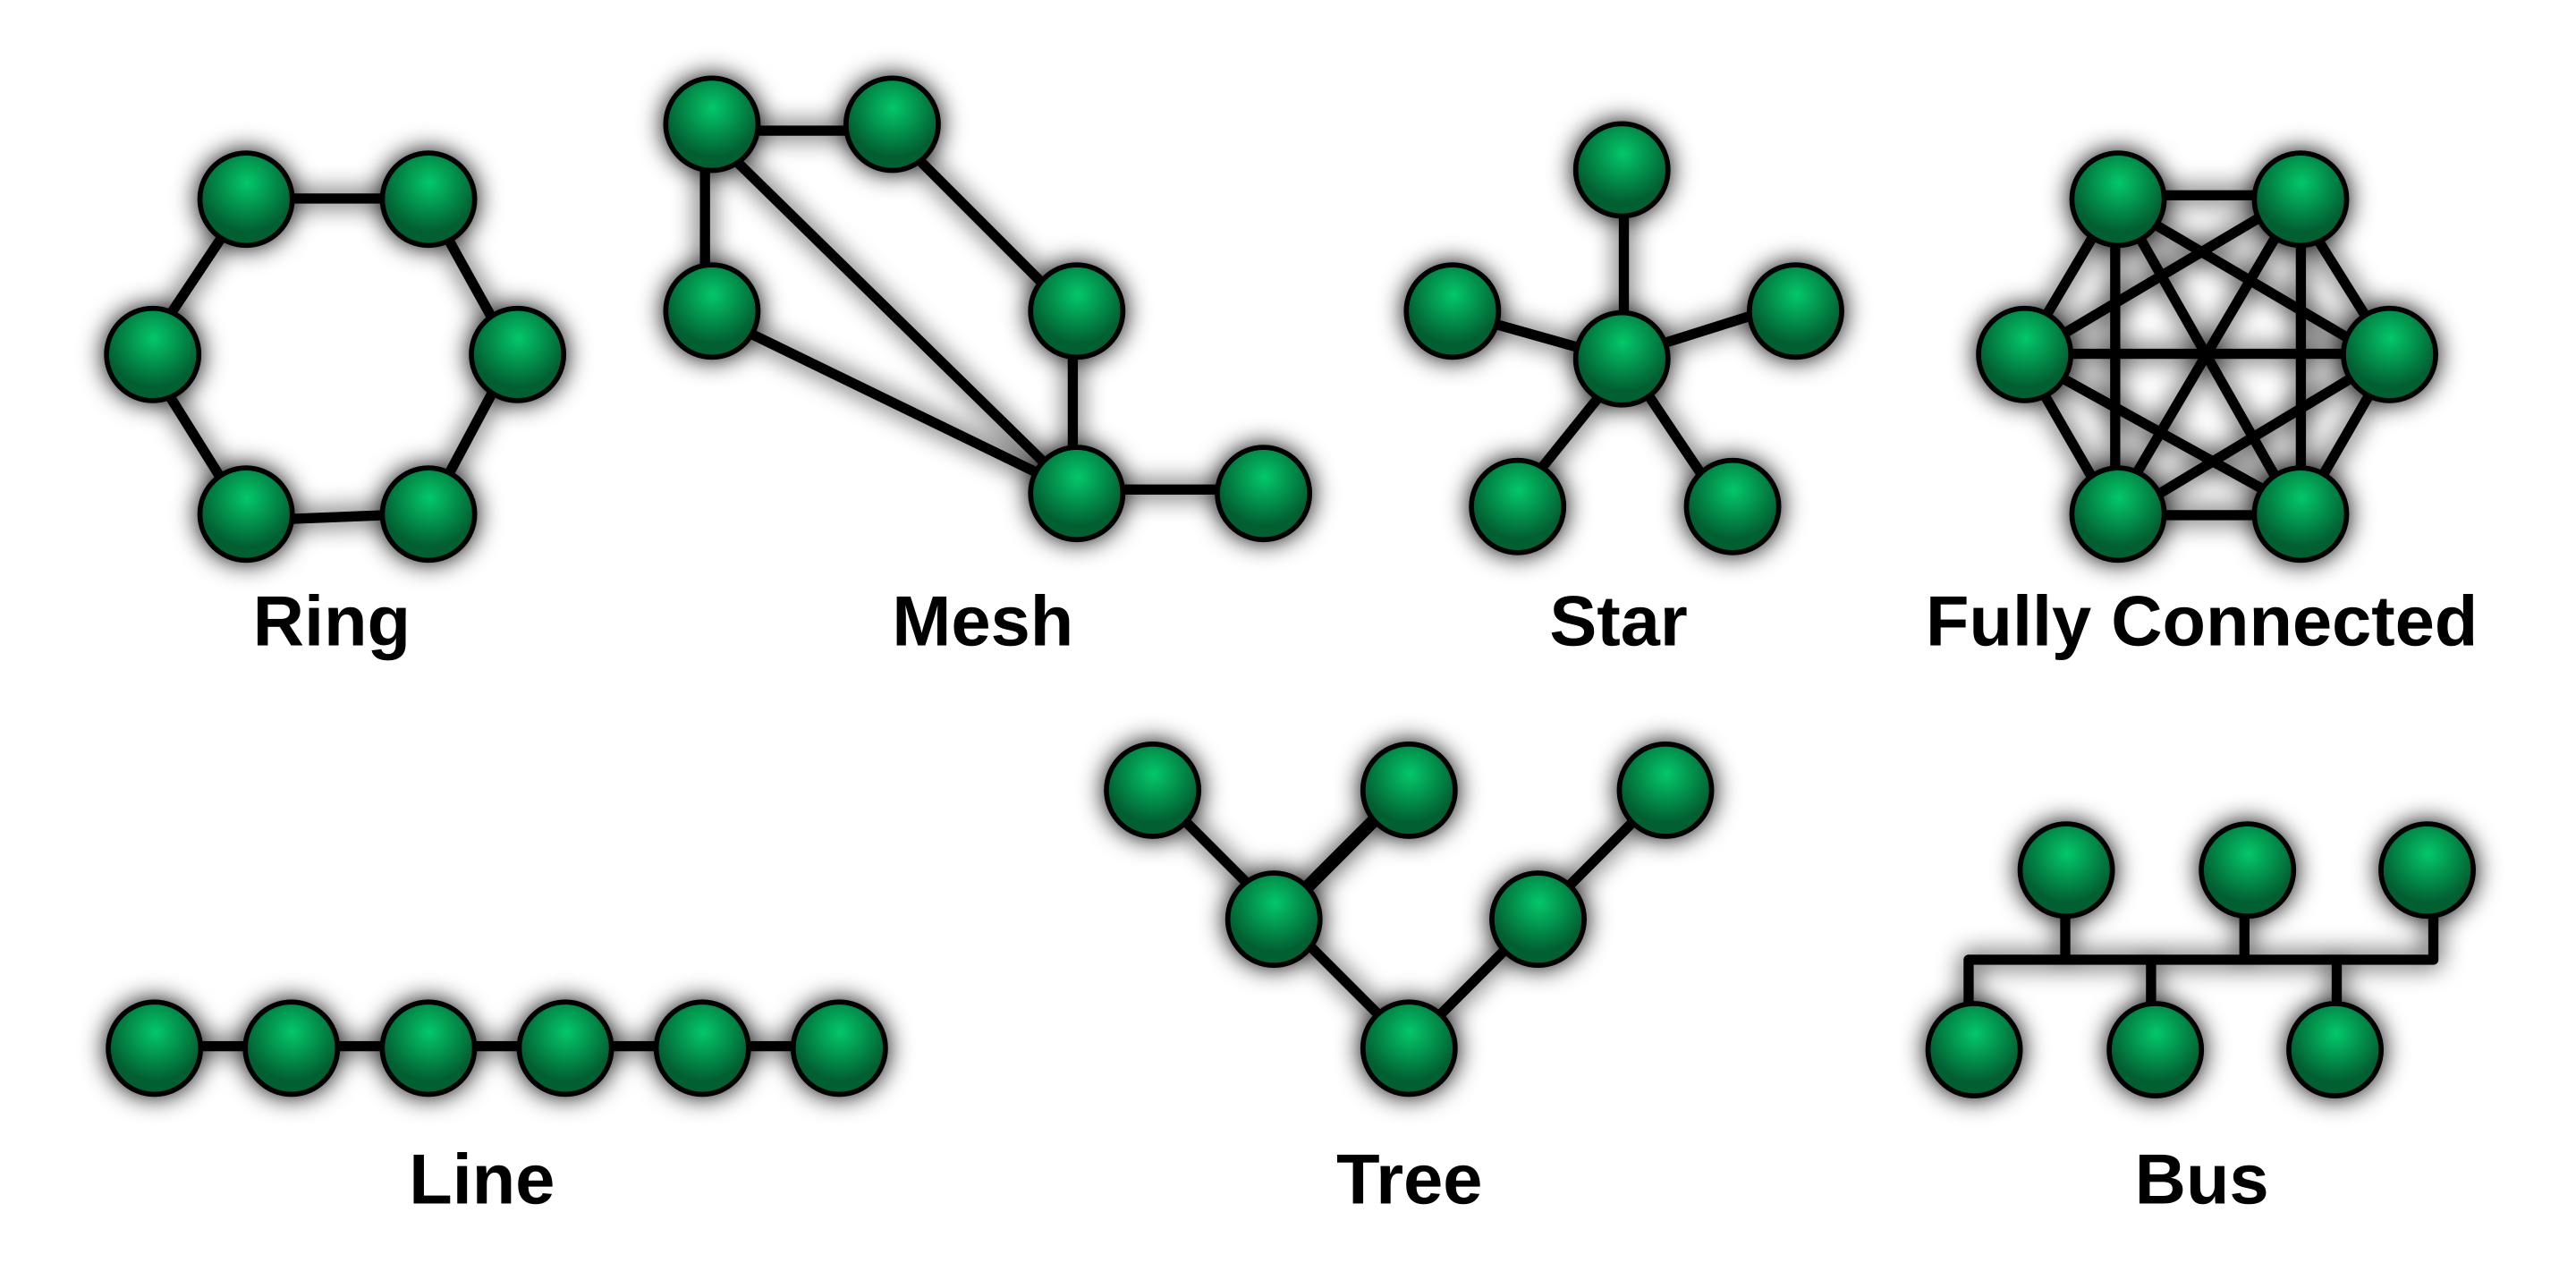
\includegraphics[width=\textwidth]{images/introduction/network-topologies.png}
\end{sidecaption}
\end{figure}



\section{Distributed computing architectures}

\emph{Distributed computing} is a field of computer science that studies distributed systems, defined as computer systems whose inter-communicating components are located on different networked computers.
We will briefly discuss two architectures, the client--server model and the peer-to-peer model.

\paragraph{client--server}
This models makes a clear distinction between the providers of resources or services, called the \emph{servers}, and the service requesters, called the \emph{clients}.
An example of the client--server model is the world-wide web with web browsers requesting the sources and the web server hosting a website, providing the service.

\paragraph{peer-to-peer}
Peers are equally-privileged participants in the network with all peers being both suppliers and consumers of resources.
An example would be the file sharing applications from yesteryear.




\section{Network evolution}
\label{sec:network-evolution}

Let's briefly examine the evolution of both local-area networks and wide-area networks.

\subsection{Local-area networks}
\label{sec:network-evolution-lan}

\paragraph{mainframe (1970)}%
   \index{mainframe}
By the early 1970s, many mainframes acquired interactive user terminals operating as time-sharing computers, supporting hundreds of users simultaneously along with batch processing.
Users gained access through keyboard or typewriter terminals%
   \index{terminal}
and specialised text terminal \gls{CRT} displays with integral keyboards, or later from personal computers equipped with terminal emulation software.

These terminals used proprietary cabling.
Replacing your mainframe with a model from a competitor thus also meant replacing all cables in the walls.
    
\paragraph{\acl{SNA} (1974)}
\Gls{SNA} is IBM's proprietary networking architecture, created in 1974.
It is a complete protocol stack for interconnecting computers and their resources.
\gls{SNA} describes formats and protocols and is, in itself, not a piece of software.
The implementation of \gls{SNA} takes the form of various communications packages, most notably \gls{VTAM}, the mainframe software package for \gls{SNA} communications.
    
\paragraph{thicknet (1980)}%
   \index{thicknet}%
   \index{10BASE5@\SC{10BASE5}}%
   \index{Ethernet!thick}%
   \index{coaxial cable}
% https://en.wikipedia.org/wiki/10BASE5
\SC{10BASE5} (also known as thick Ethernet or \emph{thicknet}) was the first commercially available variant of Ethernet.
The technology was standardised in 1982 as \acs{IEEE} 802.3.
\SC{10BASE5} uses a thick and stiff coaxial cable up to 500~metres in length.
Up to 100~stations can be connected to the cable using vampire taps and share a single collision domain with 10~Mbit/s%\SI{10}{\mega\bit\per\second}%
   \footnote{These units are often displayed as `Mbps' for megabit-per-second. In this case it is important to differentiate between a lowercase `b' for bit and an uppercase `B' for byte.}
of bandwidth shared among them.
The system is difficult to install and maintain.

\paragraph{Token Ring (1984)}%
   \index{Token Ring}%
   \index{token}
Token Ring is a computer networking technology used to build local-area networks.
It was introduced by IBM in 1984, and standardised in 1989 as \acs{IEEE} 802.5.

It uses a special three-byte frame called a \emph{token} that is passed around a logical ring of workstations or servers.
This token passing is a channel access method providing fair access for all stations, and eliminating the collisions of contention-based access methods.

Token Ring was a successful technology, particularly in corporate environments, but was gradually eclipsed by the later versions of Ethernet.

\paragraph{thinnet (1985)}%
   \index{thinnet}%
   \index{10BASE2@\SC{10BASE2}}%
   \index{Ethernet!thin}%
   \index{coaxial cable}%
   \index{connectors!BNC@\acs{BNC}}
\SC{10BASE2} (also known as cheapernet, thin Ethernet, \emph{thinnet}, and \emph{thinwire}) is a variant of Ethernet that uses thin coaxial cable terminated with \acs{BNC} connectors to build a local-area network.

During the mid to late 1980s this was the dominant Ethernet standard for 10~Mbit/s, %\SI{10}{\mega\bit\per\second}
but due to the immense demand for high speed networking, the low cost of category~5 cable, and the popularity of 802.11 wireless networks, both \SC{10BASE2} and \SC{10BASE5} have become increasingly obsolete.

\paragraph{Ethernet switches (1985)}%
   \index{switch (Ethernet)}%
   \index{bridge (Ethernet)}%
   \index{Kempf, Mark}%
   \index{collision domain}
% https://en.wikipedia.org/wiki/Network_switch
Ethernet switches are the most common form of network switch.
The first \acs{MAC} bridge was invented in 1983 by Mark Kempf, an engineer in the Networking Advanced Development group of \gls{DEC}.
The first two-port bridge product (LANBridge 100) was introduced by that company shortly after.
The company subsequently produced multi-port switches for both Ethernet and \acs{FDDI} such as GigaSwitch.
Digital decided to license its \acs{MAC} bridge patent in a royalty-free, non-dis\-crim\-i\-na\-tory basis that allowed \acs{IEEE} standardisation.
This permitted a number of other companies to produce multi-port switches, including Kalpana.
Ethernet was initially a shared-access medium, but the introduction of the \acs{MAC} bridge began its transformation into its most-common point-to-point form without a collision domain.
Switches also exist for other types of networks including Fibre Channel, \gls{ATM}, and InfiniBand.
    
\subsection{Wide-area networks}
\label{sec:network-evoluation-wan}

\paragraph{ARPAnet (1971)}%
   \index{ARPAnet}%
   \index{Telnet}%
   \iacs{FTP}%
   \index{PDP-11@\SC{PDP-11}}%
   \index{router}
The ARPAnet or Advanced Research Projects Agency network was the first wide-area packet-switched network with distributed control and one of the first networks to implement the \acs{TCP}/\acs{IP} protocol suite.
Both technologies became the technical foundation of the internet.
The first four nodes were designated as a testbed for developing and debugging the 1822 protocol, which was a major undertaking.
While they were connected electronically in 1969, network applications were not possible until the \gls{NCP}%
   \footnote{\acs{NCP} is the predecessor to \acs{TCP}.}
was implemented in 1970 enabling the first two host-to-host protocols, remote login (Telnet) and file transfer (\acs{FTP}) which were specified and implemented between 1969 and 1973.
The network was declared operational in 1971.
Network traffic began to grow once email was established at the majority of sites by around 1973.

Many of the earliest systems on the ARPAnet were \SC{PDP-11}s, see \vref{fig:thompson}.
%\footnote{\href{https://www.truecable.com/blogs/cable-academy/a-brief-history-of-network-technology}{https://www.truecable.com/blogs/cable-academy/a-brief-history-of-network-technology}}
The \SC{DECSA} communications server was a communications platform developed by \gls{DEC} based on a \SC{PDP-11/24}, with the provision for user installable \gls{IO} cards including asynchronous and synchronous modules.
This product was used as one of the earliest commercial platforms upon which networking products could be built, including \SC{X.25} gateways, \gls{SNA} gateways, routers, and terminal servers.%
\footnote{A terminal server connects devices with a serial port to a local-area network.}
Ethernet adapters were also available.

\begin{figure}
\begin{sidecaption}%
   [Thompson and Ritchie working on a \SC{PDP-11}]%
   {Ken Thompson (sitting) and Dennis Ritchie working on a \SC{PDP-11}, circa~1970. The picture was taken by Peter Hamer and the line drawing was made by \href{https://www.truecable.com/blogs/cable-academy/a-brief-history-of-network-technology}{truecable.com}.}%
   [fig:thompson]
\centering
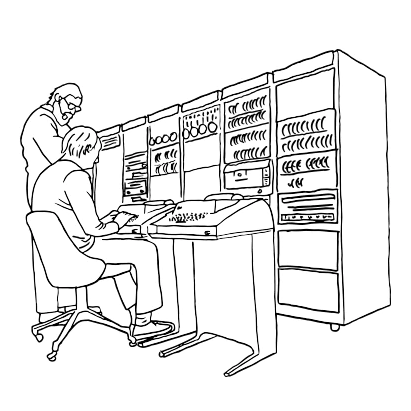
\includegraphics[width=\textwidth]{images/introduction/thompson.png}
\end{sidecaption}
\end{figure}

\paragraph{\SC{X.25} (1976)}%
   \index{X.25@\SC{X.25}}
\SC{X.25} is an \acs{ITU-T} standard protocol suite for packet-switched data communication in \aclp{WAN}.
Is is one of the oldest packet-switching communication protocols available; it was developed several years before \gls{IP} version~4 (1981) and the \gls{OSI} reference model (1984).
The protocol suite is designed as three conceptual layers, which correspond closely to the lower three layers of the seven-layer \gls{OSI} model.
It also supports functionality not found in the \gls{OSI} network layer.
% TODO: such as?
% Perhaps "The X.25 data link layer, LAPB, provides a reliable data path across a data link (or multiple parallel data links, multilink) which may not be reliable itself." (wikipedia)

\paragraph{Minitel (1984)}
   \index{Minitel}%
   \index{terminal}%
   \index{modem}
In the early 1980s the French launched the Minitel project, an ambitious plan to bring data networking into everyone's home.
Sponsored by the French government, the Minitel system consisted of a public packet-switched network, Minitel servers, and inexpensive terminals with built-in low-speed modems.
The Minitel became a huge success in 1984 when the French government gave away a free Minitel terminal to each French household that wanted one.
Minitel sites included free sites -- such as a telephone directory site -- as well as private sites, which collected a usage-based fee from each user.
At its peak in the mid 1990s, it offered more than twenty thousand services, ranging from home banking to specialised research databases.
The Minitel was in a large proportion of French homes ten years before most Americans had ever heard of the internet.

\paragraph{NSFnet (1985)}%
   \index{NSFnet}%
   \index{backbone (network)}
The NSFnet was a program of coordinated, evolving projects sponsored by the \gls{NSF} from~1985 to~1995 to promote advanced research and education networking in the United States.
The program created several nationwide backbone computer networks in support of these initiatives.
Initially created to link researchers to the \gls{NSF}-funded supercomputing centers, through further public funding and private industry partnerships it developed into a major part of the internet backbone.

The \acl{NSF} permitted only government agencies and universities to use the network until 1989 when the first commercial \acl{ISP} emerged.
By 1991, the \acs{NSF} removed access restrictions and the commercial \acs{ISP} business grew rapidly.

\paragraph{internet (1991)}%
   \index{internet}%
   \iacs{ISP}%
   \iacs{IXP}%
   \iacs{CDN}
The internet is a network interconnecting other networks in a partial mesh topology.
It consists of many \aclp{ISP}, \glspl{IXP}, \glspl{CDN}, companies, and other organisations.

\paragraph{IPsec virtual private networks (1995)}%
   \index{VPN@\acs{VPN}!IPsec}%
   \index{VPN@\acs{VPN}!MPLS@\acs{MPLS}}%
\Glspl{VPN} are private networks that run on top of a public network, either the internet in case of IPsec \gls{VPN} or the backbone of a service provider in case of \acs{MPLS} \gls{VPN}.
IPsec is used to encrypt the data sent over these virtual connections or tunnels and ensure confidentiality and integrity.

%\paragraph{MPLS virtual private networks (1999)}

\paragraph{cloud computing (2002)}%
   \index{cloud computing}
In July 2002, Amazon created subsidiary Amazon Web Services, with the goal to `enable developers to build innovative and entrepreneurial applications on their own.'
In March 2006 Amazon introduced its Simple Storage Service (\SC{S3}), followed by Elastic Compute Cloud (\SC{EC2}) in August of the same year.
These products pioneered the usage of server virtualisation to deliver IaaS at a cheaper and on-demand pricing basis.

\paragraph{YouTube (2005)}
Google launched YouTube on February 14, 2005 and was the beginning of ubiquitous video and massive amounts of user-generated content.




\section{Routing schemes}
\label{sec:ip-routing-schemes}
Routing schemes differ in how they deliver messages.
Unicast is the dominant form of message delivery on the internet.

\paragraph{unicast}
   \index{routing scheme!unicast}
Unicast is a one-to-one transmission from one point in the network to another point (\cref{fig:unicast}); that is, one sender and one receiver, each identified by a network address.


\begin{marginfigure}
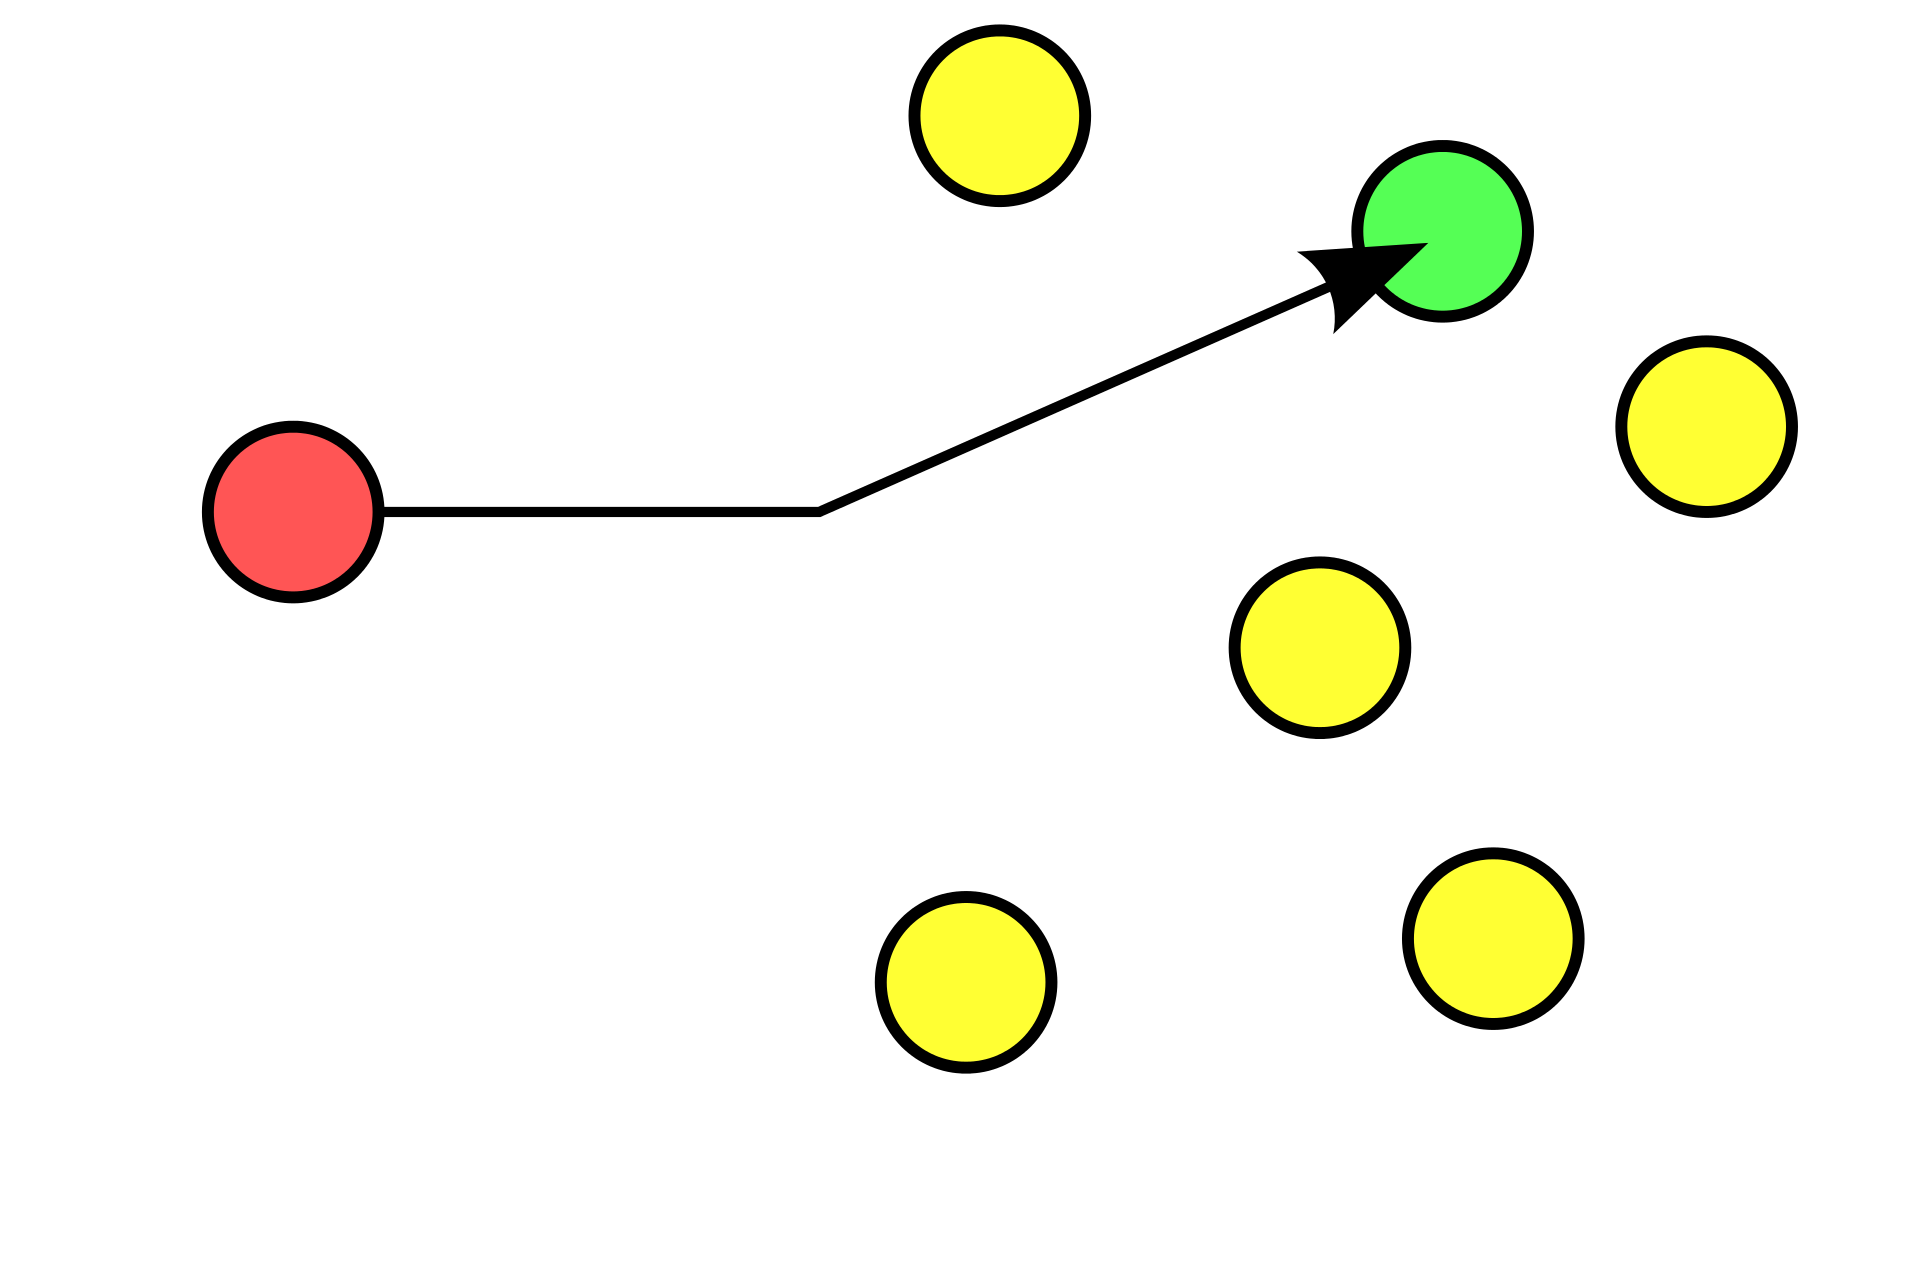
\includegraphics[width=\textwidth]{images/introduction/unicast.png}
\caption[Unicast routing scheme]{Unicast routing}
\label{fig:unicast}
\end{marginfigure}

% \begin{figure}
% \begin{minipage}{.4\textwidth}
% 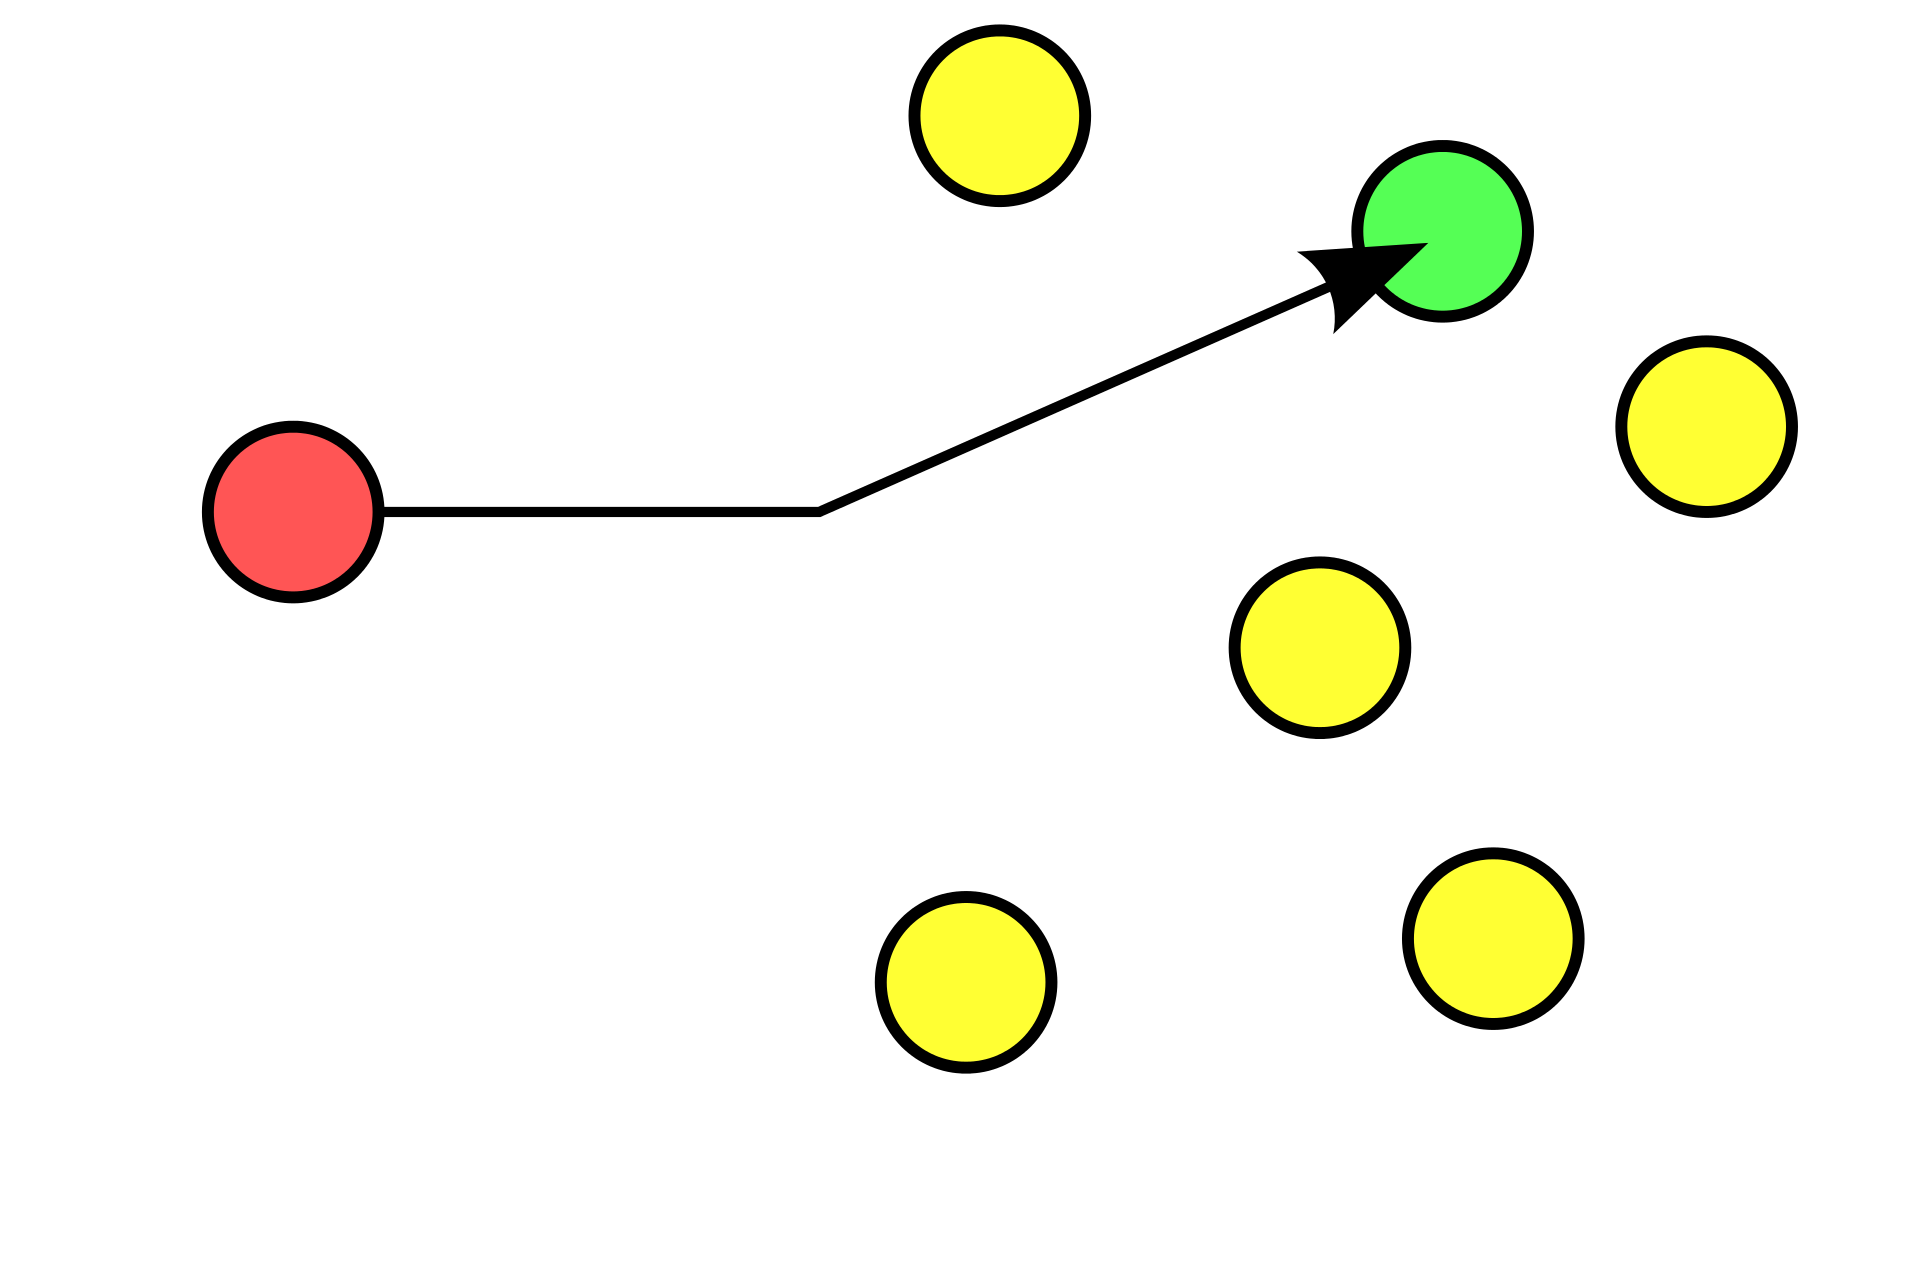
\includegraphics[width=\textwidth]{images/introduction/unicast.png}
% \caption[Unicast routing scheme]{Unicast routing}
% \label{fig:unicast}
% \end{minipage}
% \hfill
% \begin{minipage}{.4\textwidth}
% 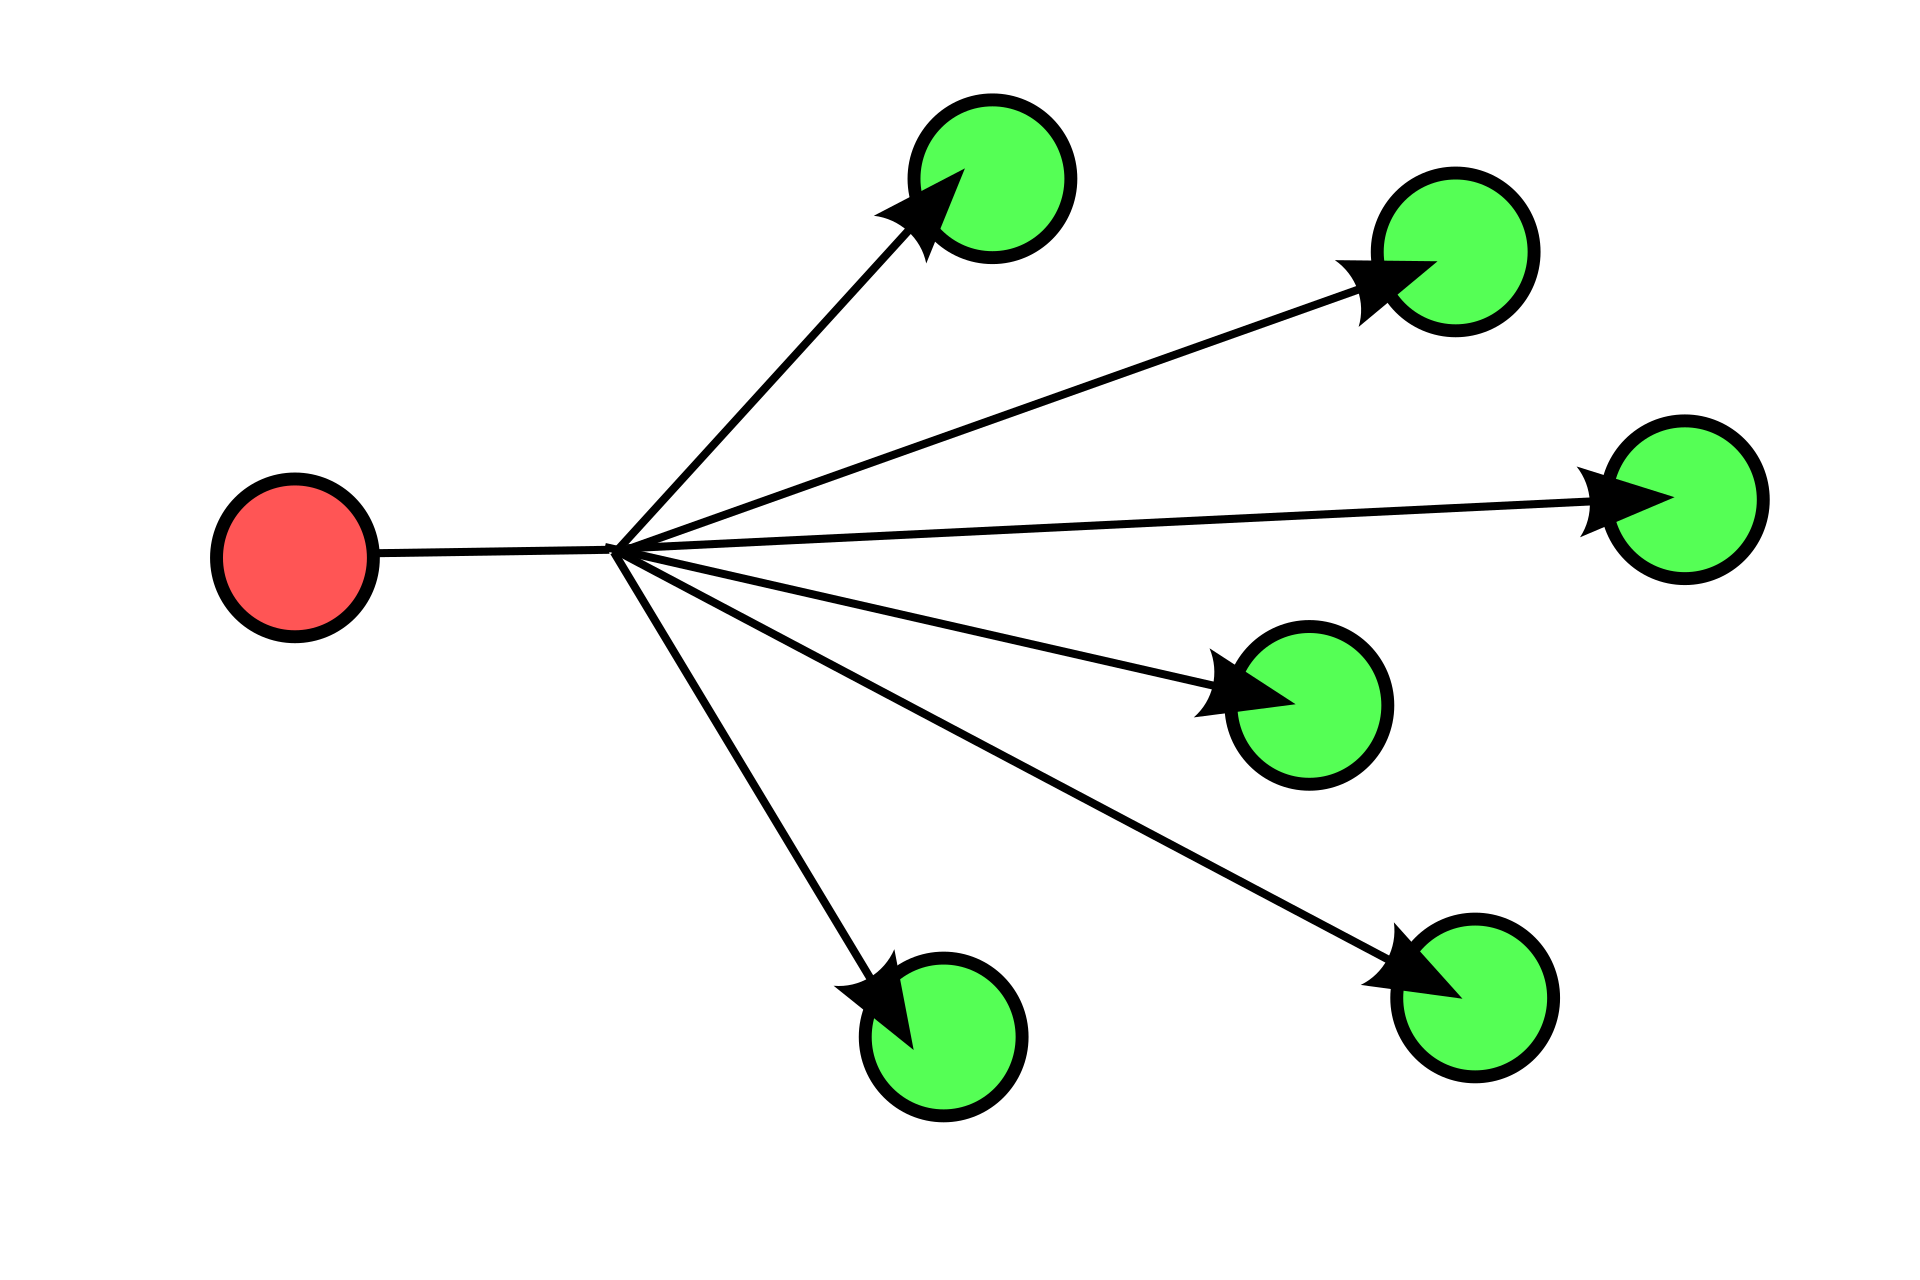
\includegraphics[width=\textwidth]{images/introduction/broadcast.png}
% \caption[Broadcast routing scheme]{Broadcast routing}
% \label{fig:broadcast}
% \end{minipage}
% \end{figure}

\paragraph{broadcast}
   \index{routing scheme!broadcast}
Broadcasting is a method of transferring a message to all recipients simultaneously (\cref{fig:broadcast}).
Broadcasting can be performed as a high-level operation in a program, or it may be a low-level networking operation, for example broadcasting on Ethernet.

\begin{marginfigure}
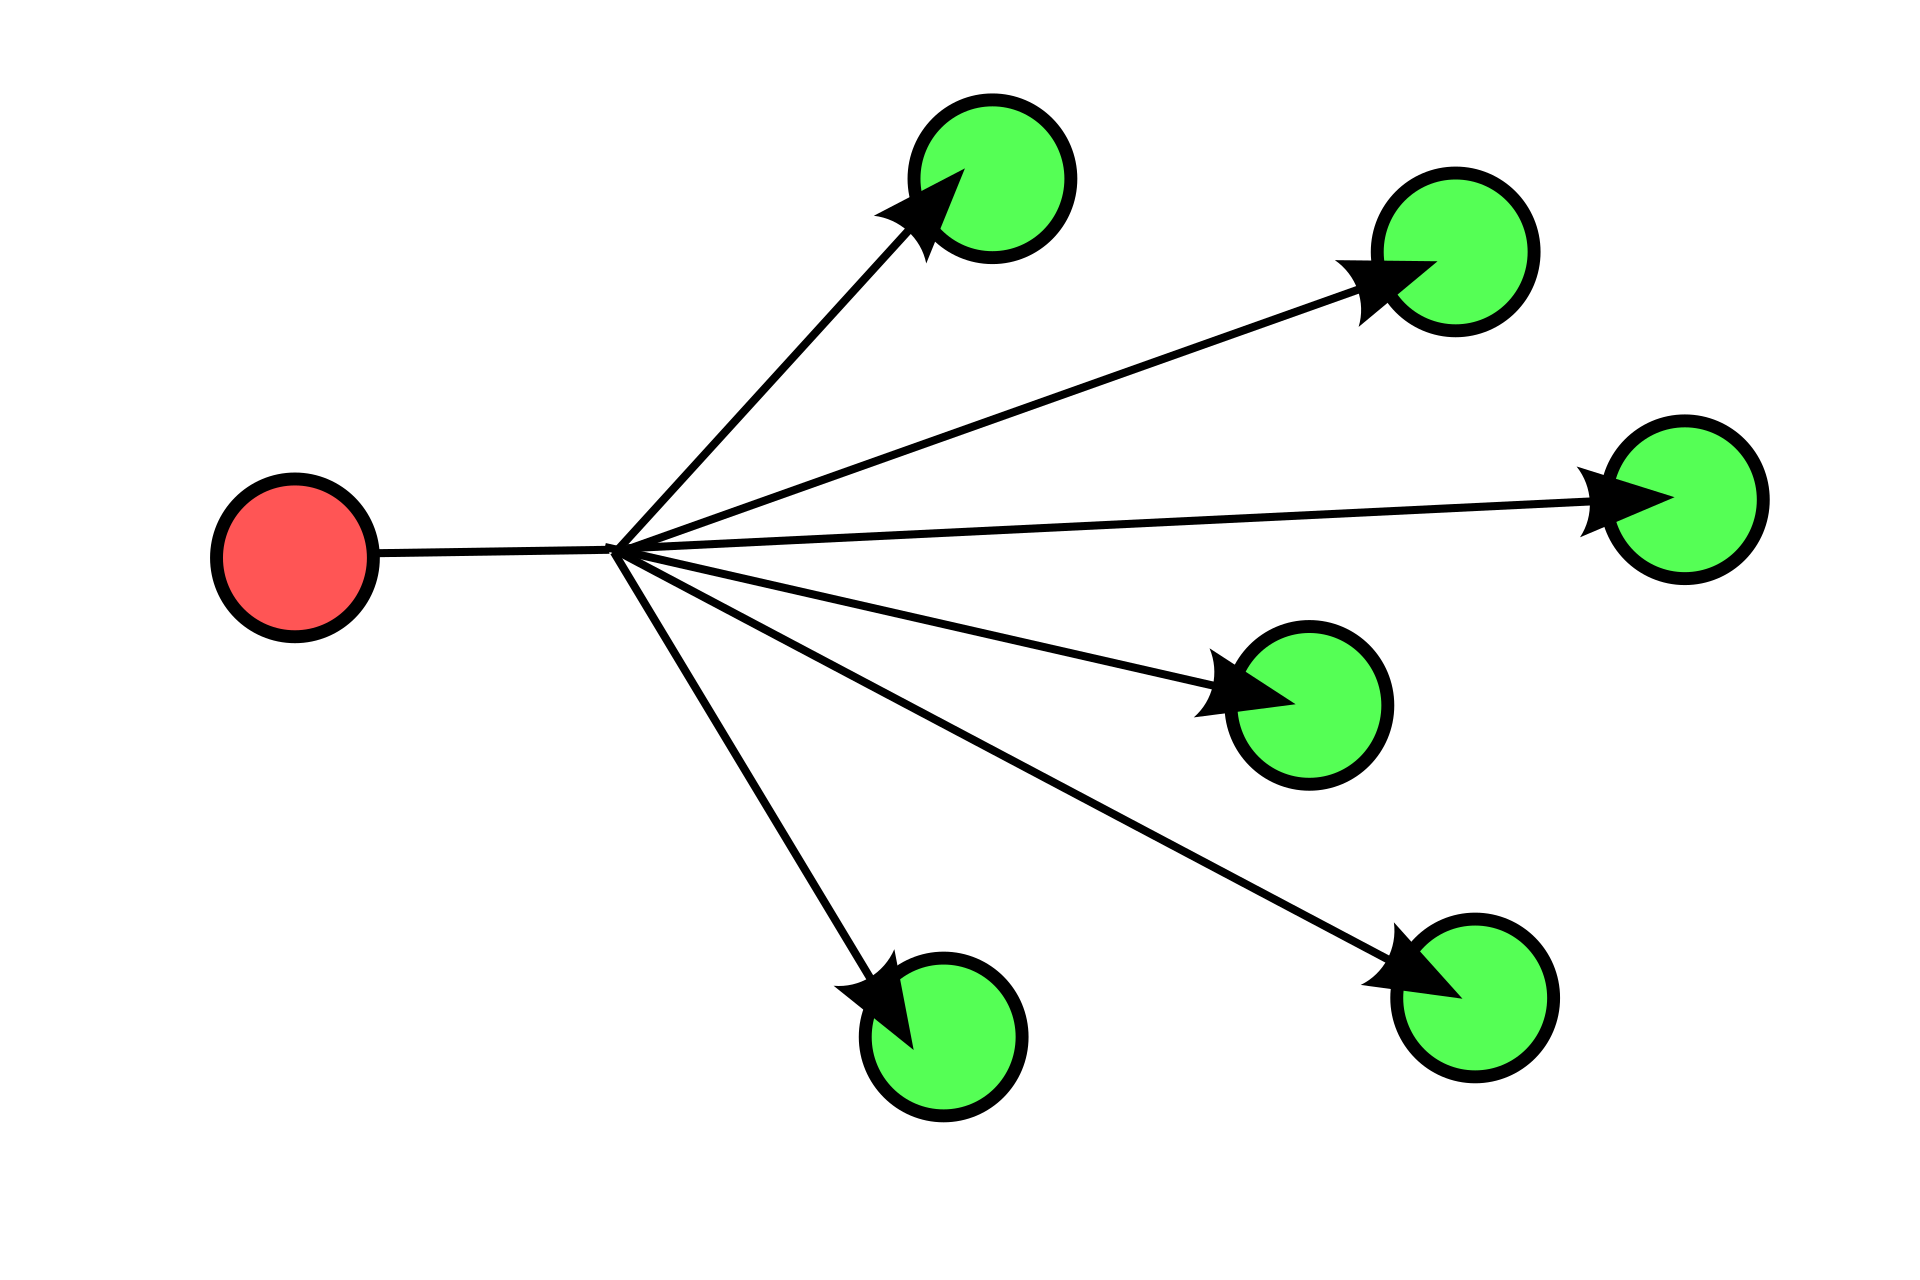
\includegraphics[width=\textwidth]{images/introduction/broadcast.png}
\caption[Broadcast routing scheme]{Broadcast routing}
\label{fig:broadcast}
\end{marginfigure}
   

\paragraph{multicast}
   \index{routing scheme!multicast}
Multicast is group communication where data transmission is addressed to a group of destination computers simultaneously (\cref{fig:multicast}).
Multicast can be one-to-many or many-to-many distribution.

\begin{marginfigure}
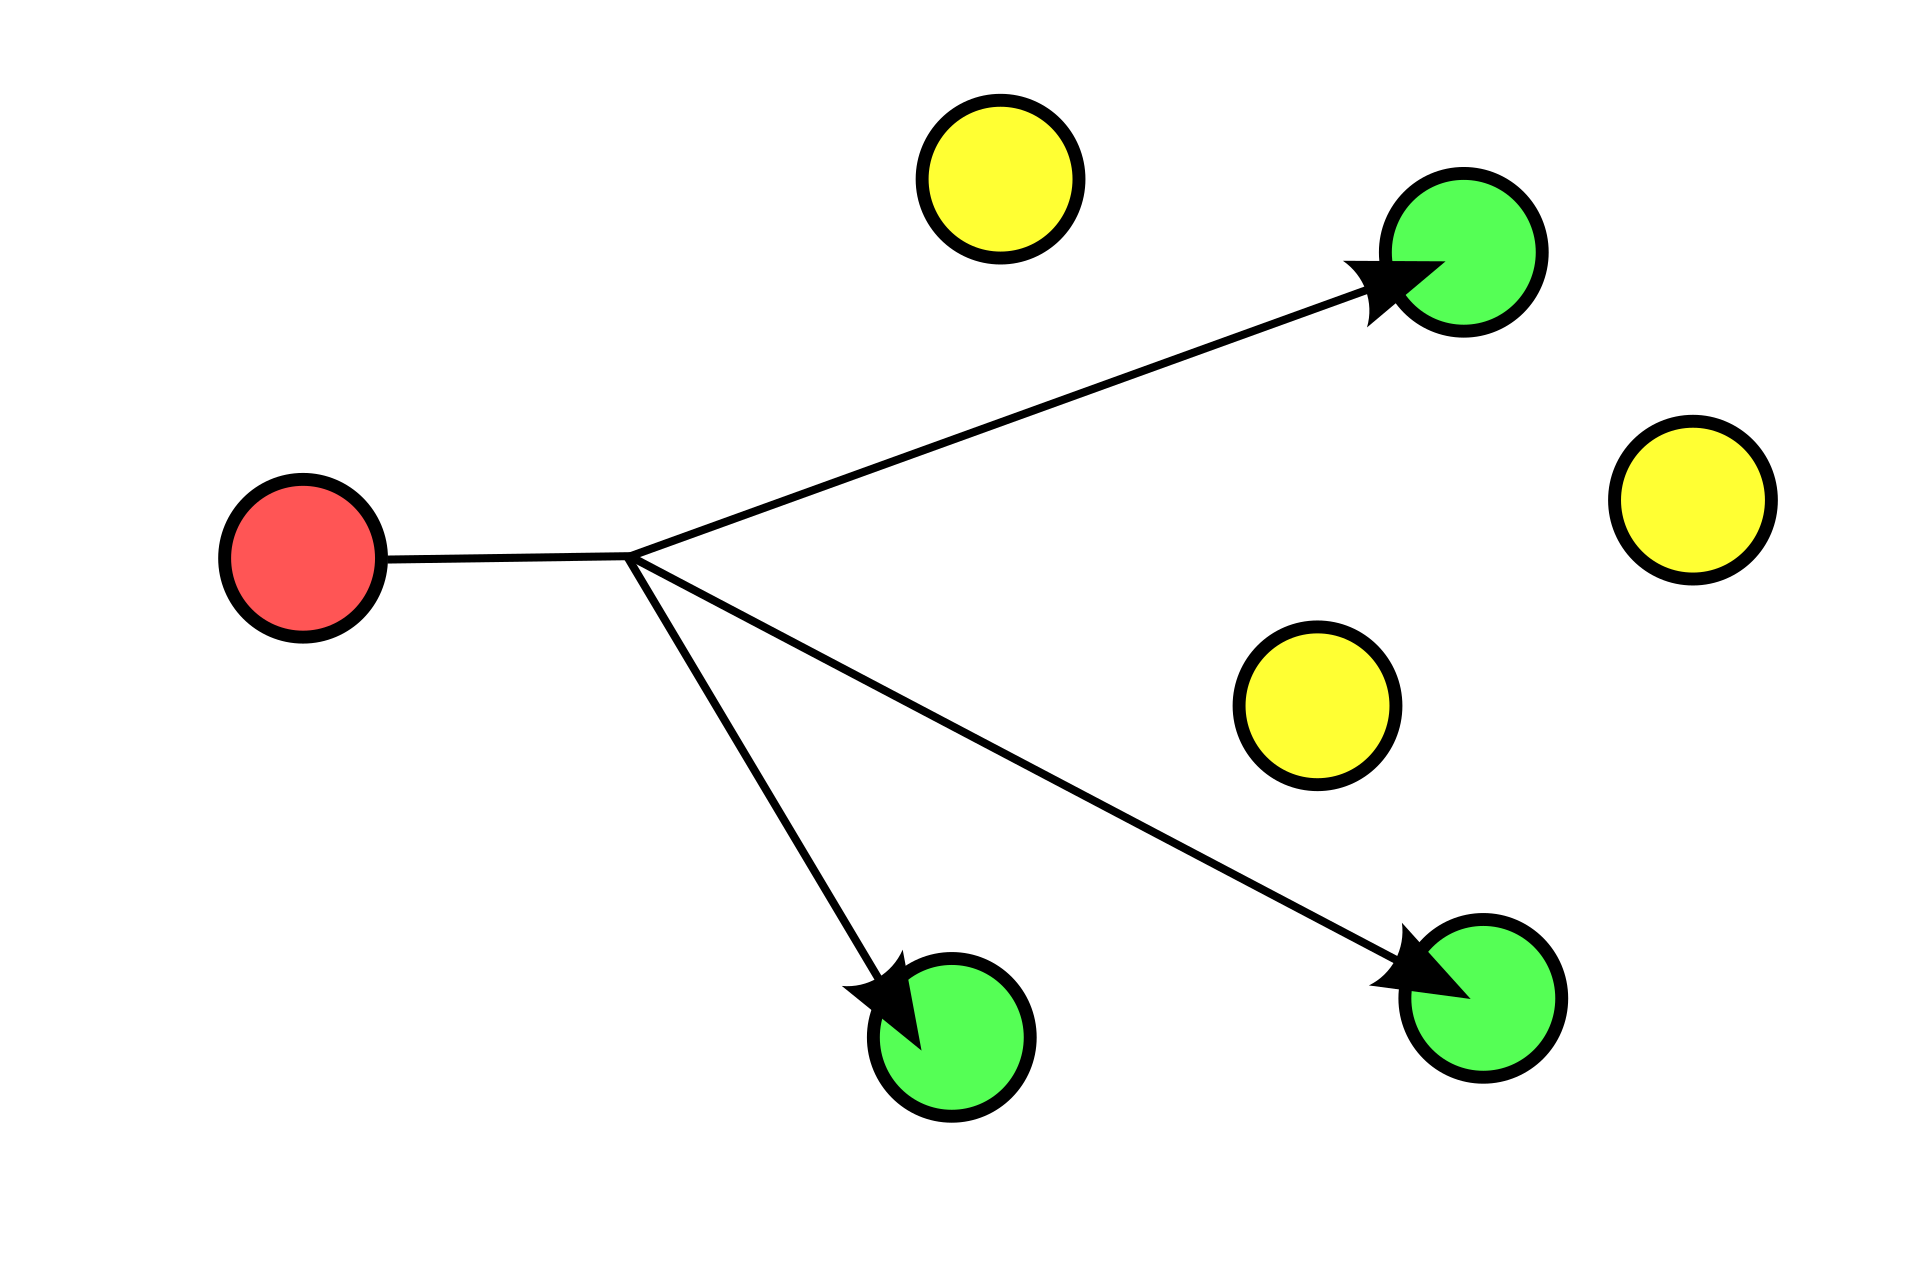
\includegraphics[width=\textwidth]{images/introduction/multicast.png}
\caption[Multicast routing scheme]{Multicast routing}
\label{fig:multicast}
\end{marginfigure}

\paragraph{anycast}
   \index{routing scheme!anycast}
   \iacs{CDN}
Anycast is a network addressing and routing methodology in which a single destination IP address is shared by devices (generally servers) in multiple locations (\cref{fig:anycast}).
Routers direct packets addressed to this destination to the location nearest the sender, using their normal decision-making algorithms, typically the lowest number of \gls{BGP} network hops.
Anycast routing is widely used by \acf{CDN} such as web and \acs{DNS} hosts, to bring their content closer to end users.

It can also be used to distribute \ac{DDoS} attacks and reduce their effectiveness.
As traffic is routed to the closest node, a process over which the attacker has no control, the \ac{DDoS} traffic flow will be distributed amongst the closest nodes.
Thus, not all nodes might be affected. 

%\begin{figure}
%\begin{minipage}{.4\textwidth}
%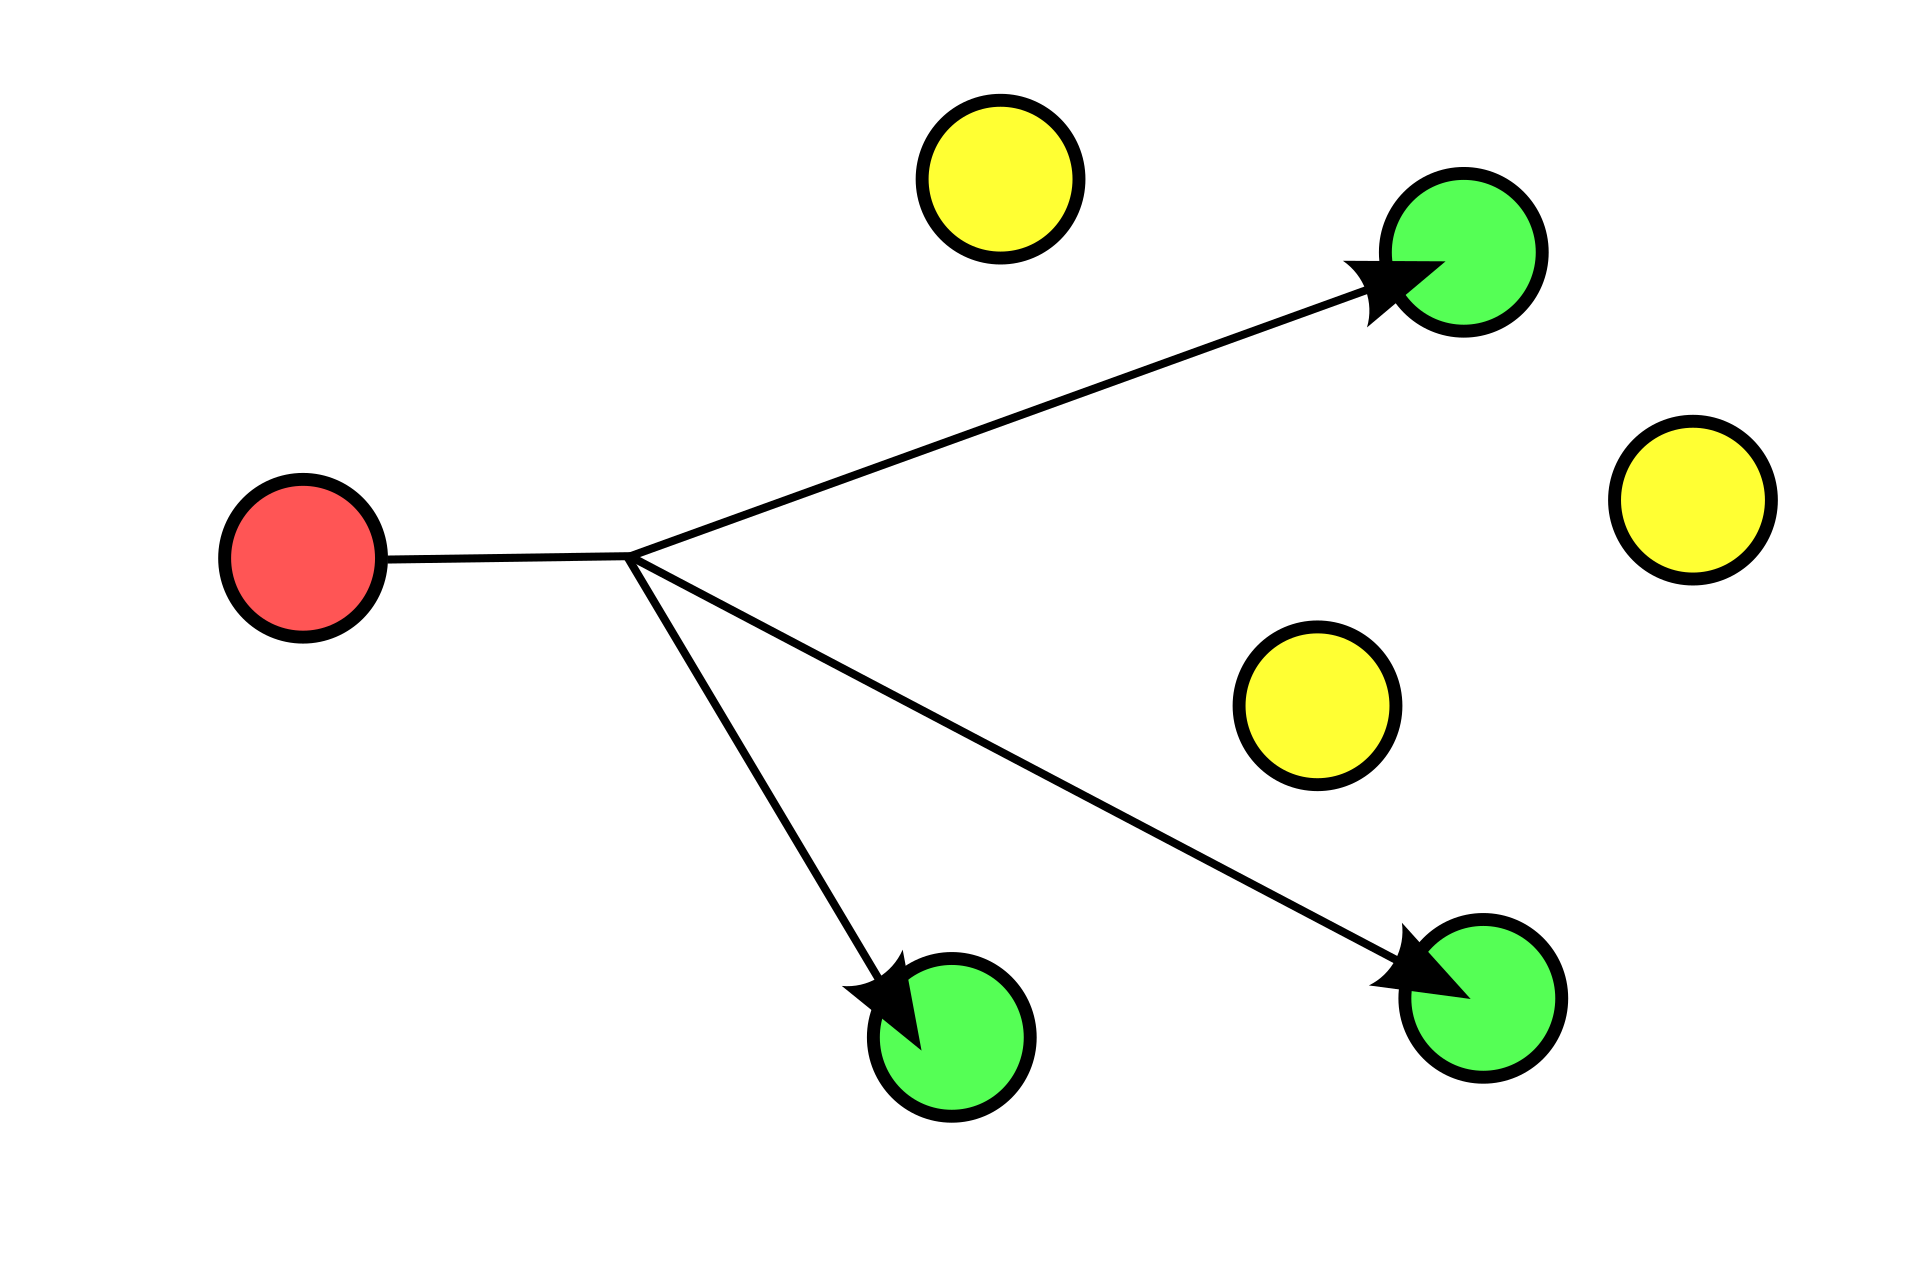
\includegraphics[width=\textwidth]{images/introduction/multicast.png}
%\caption[Multicast routing scheme]{Multicast routing}
%\label{fig:multicast}
%\end{minipage}
%\hfill
%\begin{minipage}{.4\textwidth}
%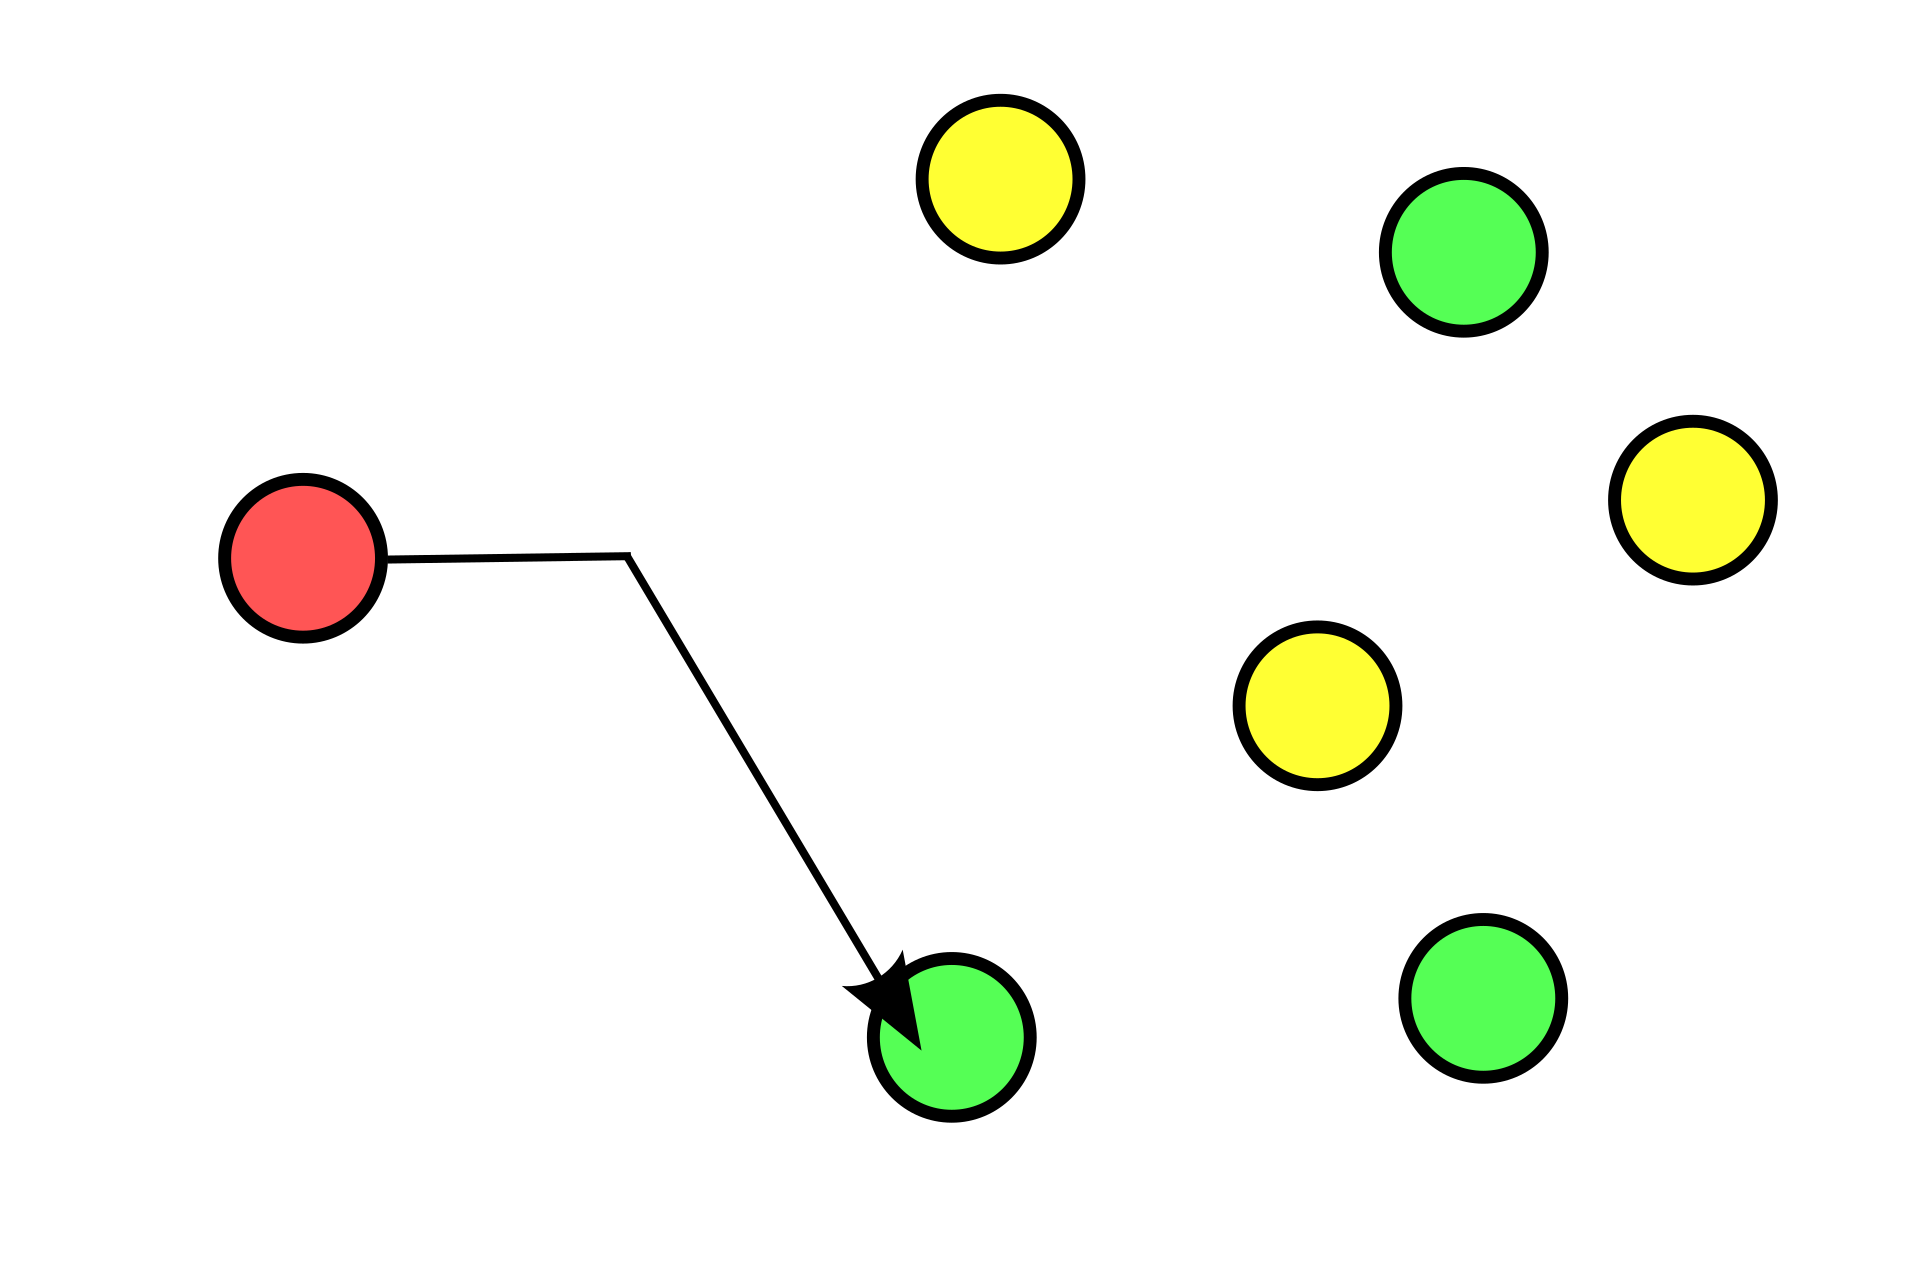
\includegraphics[width=\textwidth]{images/introduction/anycast.png}
%\caption[Anycast routing scheme]{Anycast routing}
%\label{fig:anycast}
%\end{minipage}
%\end{figure}

\begin{marginfigure}
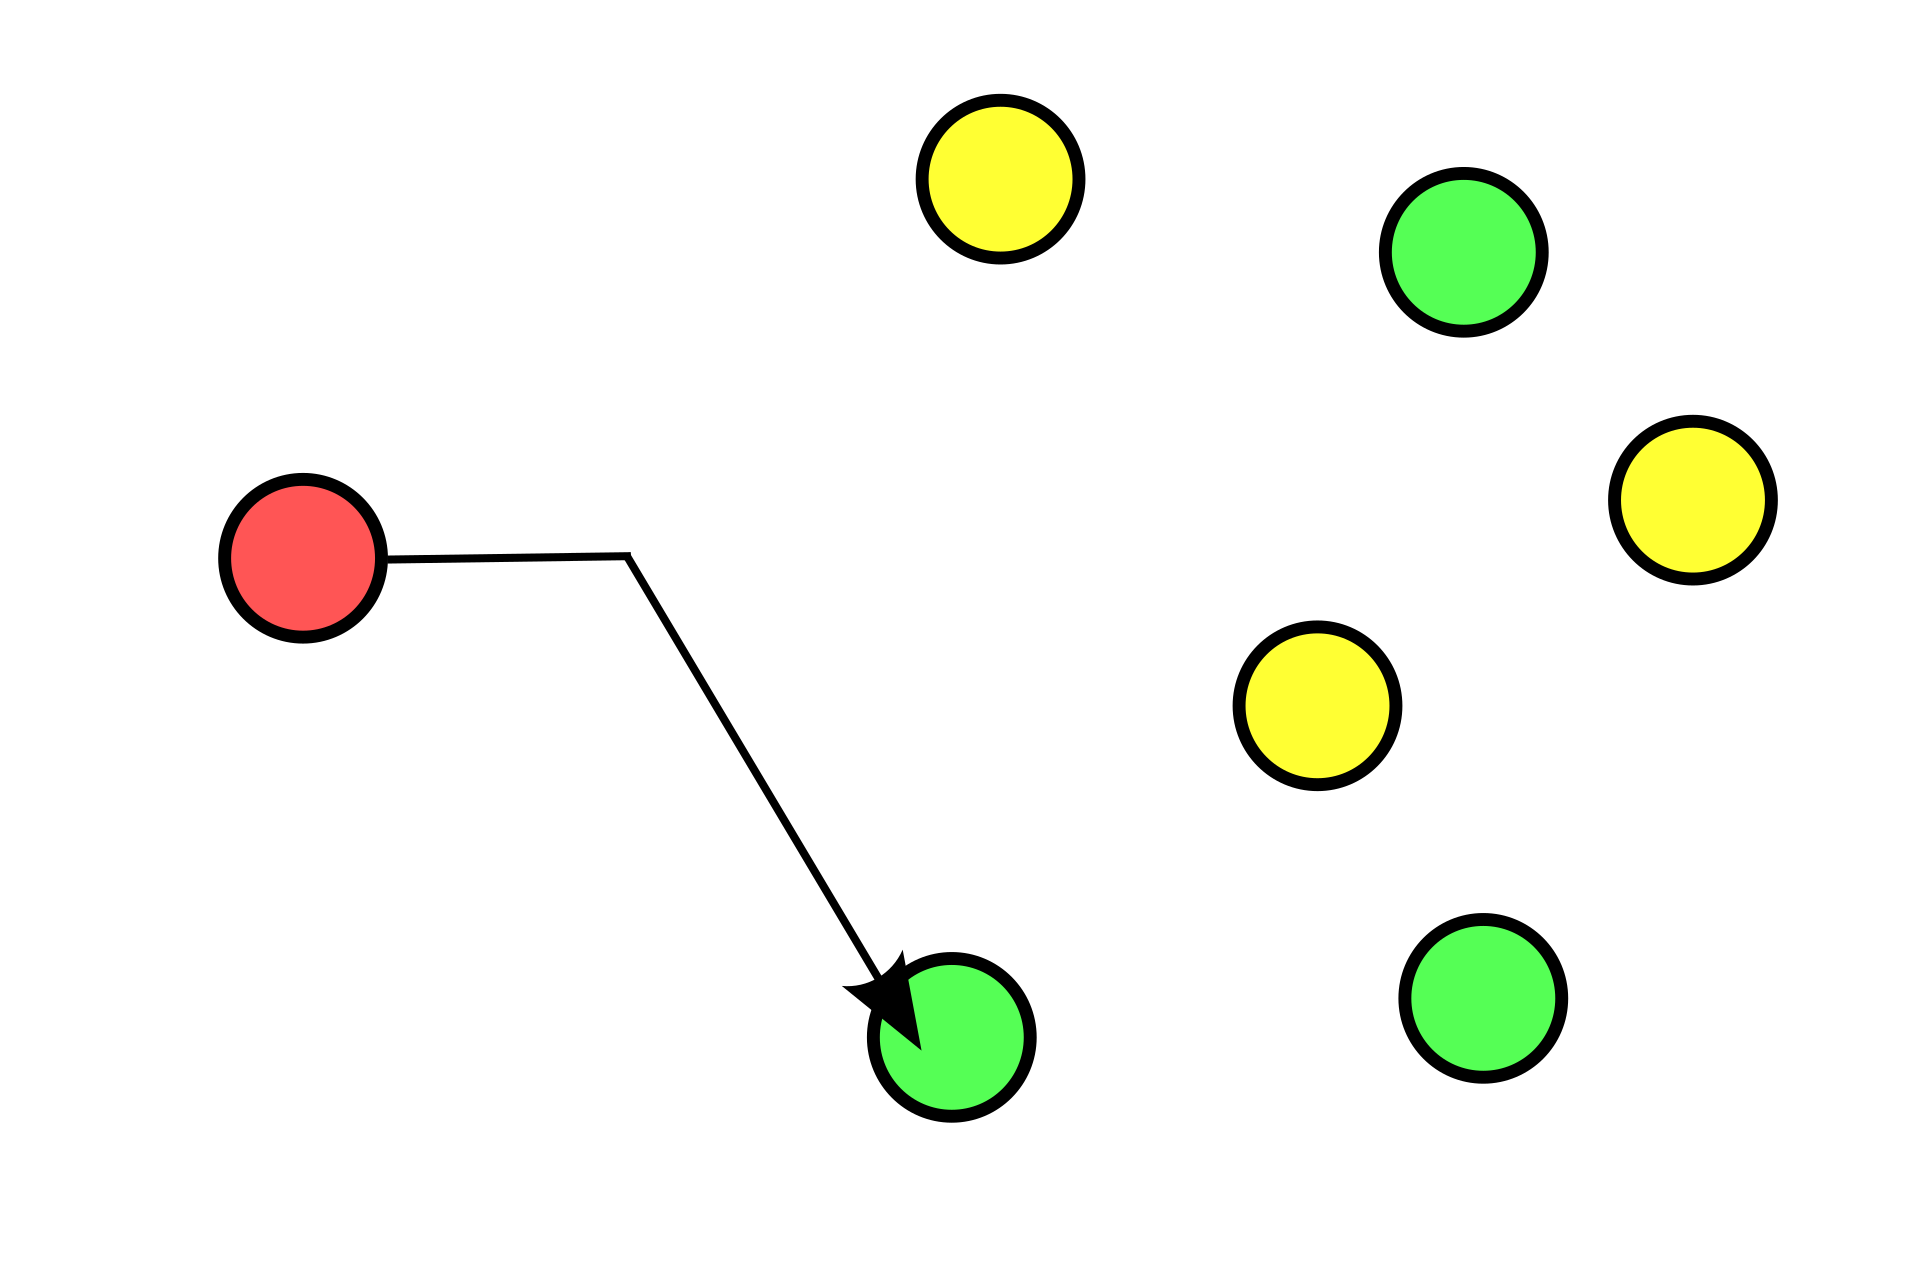
\includegraphics[width=\textwidth]{images/introduction/anycast.png}
\caption[Anycast routing scheme]{Anycast routing}
\label{fig:anycast}
\end{marginfigure}


In this course we will only cover unicast and broadcast.
Multicast and anycast are only used in very specific networks.


\section{Network models}
\label{sec:network-models}

\paragraph{\acs{OSI} model}
      \index{network model!OSI model@\acs{OSI}}
The \acf{OSI} model  (see \vref{fig:network-models}) is a conceptual model that describes the universal standard of communication functions of a telecommunication system or computing system, without any regard to the system's underlying internal technology and specific protocol suites.


\paragraph{\acs{TCP}/\acs{IP} model}
      \index{network model!TCP/IP model@\acs{TCP}/\acs{IP}}
      \index{network model!DoD@\acs{DOD}}
The \acs{TCP}/\acs{IP} model is also known as the DoD model because the development of the networking method was funded by the United States Department of Defense through \acs{DARPA}.
The \acl{IP} suite predates the \gls{OSI} model, a more comprehensive reference framework for general networking systems.


\paragraph{hybrid model}
      \index{network model!hybrid}
\textcite[53]{comer}, \textcite[129]{kozierok}, \textcite[70]{tanenbaum}, and others use a hybrid, five-layer model, which I also prefer to use.
The upper layers (session, presentation, and application) are not important for a network engineer, nor are they clearly separated.
It is advisable to keep the bottom two layers separate. The data link layer comprises Ethernet switches, and it falls under the domain of network engineers, whereas the physical layer is the responsibility of network cabling technicicans.


\begin{figure}
\begin{sidecaption}%
   [The \acs{OSI}, \acs{TCP}/\acs{IP}, and hybrid networking models]%
   {The three network models}%
   [fig:network-models]
\centering
\tikzstyle{box}=[
    minimum width=25mm,
    minimum height=8mm,
    font=\small\sffamily,
    text=black,
    node distance=8mm
]
\tikzstyle{upper}=[
    box,
    draw=spot4,
    fill=spot4!20
]
\tikzstyle{middle}=[
    box,
    draw=spot1,
    fill=spot1!20
]
\tikzstyle{lower}=[
    box,
    draw=spot2,
    fill=spot2!20
]

\begin{tikzpicture}

% OSI model
\node[upper]  (OSI7) [label=left:7.]               {application};
\node[upper]  (OSI6) [label=left:6.,below of=OSI7] {presentation};
\node[upper]  (OSI5) [label=left:5.,below of=OSI6] {session};
\node[middle] (OSI4) [label=left:4.,below of=OSI5] {transport};
\node[middle] (OSI3) [label=left:3.,below of=OSI4] {network};
\node[lower]  (OSI2) [label=left:2.,below of=OSI3] {data link};
\node[lower]  (OSI1) [label=left:1.,below of=OSI2] {physical};
\node         (OSI)  [below of=OSI1,node distance=12mm,minimum height=16mm]               {\small(\textsc{a}) OSI model};

% TCP/IP model
\node[upper]  (TCPIP4) [label=left:4.,right of=OSI6,%
                    node distance=35mm,minimum height=24mm]  {application};
\node[middle] (TCPIP3) [label=left:3.,below of=TCPIP4,
                    node distance=16mm]                      {transport};
\node[middle] (TCPIP2) [label=left:2.,below of=TCPIP3]       {internet};
\node[lower]  (TCPIP1) [label=left:1.,below of=TCPIP2,
                    node distance=12mm,minimum height=16mm]  {link};
\node         (TCPIP)  [below of=TCPIP1,node distance=16mm,minimum height=16mm]  {\small(\textsc{b}) TCP/IP model};

% hybrid model
\node[upper]  (hybrid5) [label=left:5.,right of=TCPIP4,
                    node distance=35mm,minimum height=24mm]  {application};
\node[middle] (hybrid4) [label=left:3.,below of=hybrid5,
                    node distance=16mm]                      {transport};
\node[middle] (hybrid3) [label=left:2.,below of=hybrid4]     {network};
\node[lower]  (hybrid2) [label=left:2.,below of=hybrid3]     {data link};
\node[lower]  (hybrid1) [label=left:1.,below of=hybrid2]     {physical};
\node         (hybrid)  [below of=hybrid1,node distance=12mm,minimum height=16mm]               {\small(\textsc{c}) hybrid model};
\end{tikzpicture}
\end{sidecaption}
\end{figure}


\section{Network communication}
\label{sec:network-communication}

\paragraph{How to reach the server?}
You will need the \acs{IP} address of the computer you want to communicate with.
We can get this address using the \acl{DNS} (see \vref{chap:applications}) and we can use a search engine to find the domain names of the websites we want to access.


\paragraph{Which application is the data for?}
We will use \emph{port numbers} (see \vref{chap:transport}) to indicate which application the data is for.


\paragraph{How to send a lot of data?}
   \iacs{MTU}
   \index{fragmentation}
Not all protocols allow us to send the same amount of data.
For example, Ethernet limits the packet size to 1522~bytes while \gls{ATM} had a limit of 53~bytes per packet.
This means that, depending on the protocol in use, we will have to \emph{fragment} our data in smaller pieces and the destination will need to piece back these pieces together.


\paragraph{What if something goes wrong?}
Data can get corrupted or lost in transit.
Different protocols will deal differently with these issues.
Ethernet (\vref{chap:ethernet}) only has an error detection code while \acf{TCP} (\vref{sec:tcp}) garanties correct delivery of data.


\section{Encapsulation}
\label{sec:encapsulation}

\Vref{fig:encapsulation} shows the five layers of the hybrid model and the different headers (and trailer) which get added by each layer.
When data gets send from the host on the left to the host on the right, the application passes the data to the operating system's kernel to be sent on the network.
For each layer of the protocol stack a header gets added so that the corresponding layer on the receiver's side knows what the data is for.
That is, the transport layer on the sender's side communicates with the transport layer on the receiver's side and the network layer on the sender's side communicates with the corresponding layer on the receiver's side.

\begin{figure}
\begin{sidecaption}%
   [Encapsulation and decapsulation of packets]{%
   Data encapsulation at the source and decapsulation at the destination.
   Each layer adds its own header, but the data link layer also adds a trailer.
   }%
   [fig:encapsulation]
\centering
\tikzstyle{layer}=[
    minimum width=25mm,
    minimum height=8mm,
    inner sep=0mm,
    font=\small\sffamily,
    text=black,
    node distance=12mm,
    draw=spot1,
    fill=spot1!20
]
\tikzstyle{arrow}=[->,>=stealth',semithick]
\tikzstyle{red arrow}=[arrow,very thick,spot2]
\tikzstyle{packet data}=[
    rectangle,
    draw=spot4,
    fill=spot4!20,
    text=black,
    thin,
    minimum height=8mm,
    minimum width=12mm,
    inner sep=0mm
]
\tikzstyle{packet header}=[
    rectangle,
    draw=spot5,
    fill=spot5!20,
    text=black,
    thin,
    node distance=8mm,
    minimum size=8mm,
    inner sep=0mm
]
\begin{scaletikzpicturetowidth}{\textwidth}
\begin{tikzpicture}[scale=\tikzscale]

% two network stacks
\node[layer] (a1)               {application};
\node[layer] (t1) [below of=a1] {transport};
\node[layer] (n1) [below of=t1] {network};
\node[layer] (d1) [below of=n1] {data link};
\node[layer] (p1) [below of=d1] {physical};

\node[layer] (a2) [right of=a1,node distance=90mm]  {application};
\node[layer] (t2) [below of=a2]                     {transport};
\node[layer] (n2) [below of=t2]                     {network};
\node[layer] (d2) [below of=n2]                     {data link};
\node[layer] (p2) [below of=d2]                     {physical};

\draw[arrow] (a1) -- (t1);
\draw[arrow] (t1) -- (n1);
\draw[arrow] (n1) -- (d1);
\draw[arrow] (d1) -- (p1);

\draw[arrow] (t2) -- (a2);
\draw[arrow] (n2) -- (t2);
\draw[arrow] (d2) -- (n2);
\draw[arrow] (p2) -- (d2);

\draw[red arrow] (a1) to node[packet data] {data} (a2);
\draw[red arrow] (t1) to node[packet data] (dt) {data}
                         node[packet header,left of=dt,node distance=10mm] {t}
                         (t2);
\draw[red arrow] (n1) to node[packet data] (dn) {data}
                         node[packet header,left of=dn,node distance=10mm] (hn1) {t} node[packet header,left of=dn,node distance=18mm] (hn2) {n}
                         (n2);
\draw[red arrow] (d1) to node[packet data] (dd) {data}
                         node[packet header,left of=dd,node distance=10mm] (hd1) {t} node[packet header,left of=dd,node distance=18mm] (hd2) {n} node[packet header,left of=dd,node distance=26mm] (hd3) {d} node[packet header,right of=dd,node distance=10mm] (td) {d}
                         (d2);
\end{tikzpicture}
\end{scaletikzpicturetowidth}
\end{sidecaption}
\end{figure}

The data combined with the transport layer header is called a \emph{segment};
a segment and the network layer header is called a \emph{packet};
a packet and the data link header and trailer is called a \emph{frame}.

\paragraph{port numbers}
The segment header at the transport layer adds port numbers to indicate which application the data is destined for and which application the data came from.


\paragraph{\acs{IP} addresses}
The packet header at the network layer adds \acs{IP} addresses indicating which host the data is destined for and which host it came from.


\paragraph{\acf{DNS}}
\acs{DNS} is used to find the \acs{IP} address of the destination host.
See \vref{chap:applications} for more details.


\paragraph{\acs{MAC} addresses}
At the data link layer \acs{MAC} addresses are added to the frame header.
They are used to deliver the frame on the local network.
See \vref{chap:ethernet} for further details.

\paragraph{\acf{ARP}}
The \acl{ARP} is used to translate \IP\ addresses into \acs{MAC} addresses required for communication on the local network.
We will discuss this protocol in \vref{chap:ethernet}.
%Note that these \acs{MAC} addresses are only used on Ethernet networks; Frame Relay uses addresses known as \acf{DLCI}.
%Token Ring also uses \acs{MAC} addresses.
%   \index{Frame Relay}

\section{Review questions}
\begin{enumerate}
\item
   In which of the following routing schemes, there is only one receiver?
   \begin{multicols}{2}
   \begin{enumerate}
   \item broadcast
   \item anycast
   \item unicast
   \item multicast
   \end{enumerate}
   \end{multicols}
\item
   Which of the following are layers in the \acs{TCP}/\IP\ model?
   Select three options.
   \begin{multicols}{2}
   \begin{enumerate}
   \item application
   \item internet
   \item session
   \item transport
   \item data link
   \item physical
   \end{enumerate}
   \end{multicols}
\item
   When data is encapsulated, which is the correct order?
   \begin{enumerate}
   \item data, frame, packet, segment, bit
   \item segment, data, packet, frame, bit
   \item data, segment, packet, frame, bit
   \item data, segment, frame, packet, bit
   \end{enumerate}
\item
   Both an Ethernet hub and a Token Ring \acs{MAU} have a central device to which all computers connect.
   Both have thus a physical star topology.
   Why does the hub have logical bus topology while the \acs{MAU} has a logical ring topology?
\end{enumerate}

\section{Practice questions}
\begin{enumerate}
\item
   When writing software or configuraton network services, you can often use the protocol name instead of the \acs{TCP} or \acs{UDP} port number.
   The operating system needs to translate this name into a number and uses a lookup table for this.
   On Unix-based system you can find this file in \emph{/etc/services};
   on Windows this file is located in \emph{C:\textbackslash{}Windows\textbackslash{}System32\textbackslash{}drivers\textbackslash{}etc\textbackslash{}services}.
   Open this file with a text editor and look up the port numbers used by \acs{HTTP} and \acs{SSH}.
\end{enumerate}
\chapter{Internet Protocol}
\label{chap:ip}

\section{\acs{IP} addresses}
\label{sec:ip-addresses}
   
\paragraph{32 bits}
An \acs{IP} version~4 address is a 32-bit number meaning the computer uses 32~bits or four octets to store the \acs{IP} version~4 address in memory.
What these four octets mean, depends on how we want to interpret them.
For example, the following 32~bits can be interpreted as the number \numprint{1113945185}.%
   \footnote{You can also interpret these four octets as the string `Beta' when using the \acs{ASCII} character table for the conversion.}
\begin{center}
\lstinline{0100 0010}\quad\lstinline{0110 0101}\quad\lstinline{0111 0100}\quad\lstinline{0110 0001}
\end{center}     

\paragraph{four octets}
   \index{octet}
To make this 32-bit number more manageable to humans, we group the 32 bits into four sets of eight bits, called \emph{octets}.%
\footnote{%
   Currently all bytes are also eight bits so the words octet and byte are interchangeable.
   However, the size of the byte has historically been hardware-dependent and no definitive standards existed that mandated the size.
   Sizes from 1~to~48 bits have been used.
   For example, the \SC{PDP-7}, a predecessor of the \SC{PDP-11}, was an 18-bit machine.\index{PDP-07@\SC{PDP-7}}\index{PDP-11@\SC{PDP-11}}
}
\begin{center}
$\underbrace{\mbox{\lstinline{0100 0010}}}_{\mbox{octet 1}}$\quad%
$\underbrace{\mbox{\lstinline{0110 0101}}}_{\mbox{octet 2}}$\quad%
$\underbrace{\mbox{\lstinline{0111 0100}}}_{\mbox{octet 3}}$\quad%
$\underbrace{\mbox{\lstinline{0110 0001}}}_{\mbox{octet 4}}$
\end{center} 

\paragraph{dotted decimal}
   \index{dotted decimal}
We then convert these octets into decimal and separate the four octets with a dot.
This turns the number \numprint{1113945185} into the more human-friendly format 66.101.116.97.
Each of these four numbers is an octet (eight bits) to the computer.
The lowest value is 0 when all bits are zero and the highest possible value is 255 when all eight bits are set to one.%
   \footnote{%
      We can use a bit of mathematics here.
      Each bit has two possible values, 0 or 1.
      Eight bits then give us $2^8 = 256$ possible combinations or the values from 0 to 255.
      The format of an \acs{IP} address thus is $x_1.x_2.x_3.x_4$ with $x_i \in [0,255]$.
   }

It is important to remember that these \acs{IP} addresses are still just numbers to the computer and thus one \acs{IP} address is either higher or lower than a second address.
If you add 1 to the address 10.149.12.251, you get the next address, being 10.149.12.252.
If you add 1 to the address 10.149.12.255, you get the address 10.149.13.0, and adding 1 to the \acs{IP} address 10.149.255.255 gives the address 10.150.0.0.

\paragraph{hierarchy}
Similar to a street address, \acs{IP} addresses also have an hierarchy.
While a street address is structured as country, city, street, and house number, an \acs{IP} address is structured using \emph{supernetting}, \emph{subnetting}, and the division between the network and the host part.

\paragraph{network part}
Each \acs{IP} address consists of two parts.
The first, left, part uniquely identifies the local network to which the address belongs.
This is the network part or \emph{network number}.%
   \index{network number}
All computers attached to the same local network need an \acs{IP} address with the same network number.

\begin{margintable}
\footnotesize
\begin{tabular}{@{}rl@{.}r@{}}
\textcolor{spot5}{\acs{IP} address} & \textcolor{spot1}{192.0} & \textcolor{spot2}{2.7} \\
\textcolor{spot5}{subnet mask}      & 255.255                  & 0.0                    \\
\textcolor{spot5}{network number}   & \textcolor{spot1}{192.0} &                        \\
\textcolor{spot5}{host identifier}  &                          & \textcolor{spot2}{2.7} \\
\end{tabular}
\caption{The subnet mask determines where to split the \acs{IP} address into its network number and host identifier}
\label{tab:network-host-part}
\end{margintable}

\paragraph{host part}
The \emph{host identifier}%
   \index{host identifier}
is the second part, on the right of the network number, which uniquely identifies the node on the network.

\paragraph{subnet mask}
   \index{subnet mask}
The subnet mask is also a 32-bit number consisting of two parts.
Starting from the left, there is a set of ones for the network part of the \acs{IP} address.
This is followed by a set of zeros for the host part.
For example, the subnet mask 255.255.255.0 consists of 24 ones followed by eight zeros.
This means that the first 24 bits -- or first three octets -- indicate the network, while the last 8 bits are used to uniquely identify hosts within the network.
This means there can be up to $2^8=256$ hosts in the network.
\Vref{tab:network-host-part} uses a subnet mask with 16 ones and 16 zeros.
This allows for a total of $2^{16}=65536$ hosts in that network.

\begin{margintable}
\footnotesize
\begin{tabular}{
   @{}r
   p{5mm}@{ }
   p{4mm}@{ }
   p{4mm}@{ }
   p{4mm}@{ }
   p{3mm}@{ }
   p{3mm}@{ }
   p{3mm}@{ }
   p{3mm}@{}
}
value & 128 & 64 & 32 & 16 & 8 & 4 & 2 & 1 \\
\midrule
  255 &   1 &  1 &  1 &  1 & 1 & 1 & 1 & 1 \\
   99 &   0 &  1 &  1 &  0 & 0 & 0 & 1 & 1 \\
   61 &   0 &  0 &  1 &  1 & 1 & 1 & 0 & 1 \\
\end{tabular}
\caption{A few decimal numbers and their binary representation}
\end{margintable}

\paragraph{prefix length}
   \index{prefix!length}
The prefix length is the size of the prefix in number of bits.
It translates directly to the subnet mask.
The prefix length is the number of ones in the subnet mask.
The subnet mask 255.255.255.0 contains 24 ones followed by eight zeros.
The prefix length thus is 24.
A second example could be 255.255.255.192.
Converting these octets to binary gives us 26 consecutive ones followed by 6 zeros.
This means that the first 26~bits of the accompanying \acs{IP} address are the network number and the last six bits are the host identifier.

\paragraph{prefix}
   \index{prefix}
The network prefix is the first part of the \acs{IP} address, identifying the network.
The term is often used interchangeably with \emph{network address} but technically the prefix is only the network part.

\paragraph{network address}
   \index{network address}
Each network requires two special addresses that can not be assigned to hosts.
The first is the network address.
It is the first \acs{IP} address in the network, i.e.~the \acs{IP} address where the host part consists of only zeros.

\begin{margintable}
\footnotesize
\begin{tabular}{@{}rl@{.}r@{}}
\textcolor{spot5}{\acs{IP} address}  & \textcolor{spot1}{198.51.100}  & 13 \\
\textcolor{spot5}{subnet mask}       & 255.255.255 &  0 \\
\textcolor{spot5}{network addr.}     & \textcolor{spot1}{198.51.100}  & \textcolor{spot2}{0}   \\
\textcolor{spot5}{broadcast addr.}   & \textcolor{spot1}{198.51.100}  & \textcolor{spot2}{255} \\
\end{tabular}
\caption{The network address is the first address, the broadcast address is the last address}
\label{tab:network-broadcast-address}
\end{margintable}

Let's take the \acs{IP} address 198.51.100.13 as an example, using the subnet mask 255.255.255.0.
As there are 24~ones, the first 24~bits -- or three octets -- of the \acs{IP} address are the network number.
The last 8~bits of the subnet mask are zero so the last octet of the \acs{IP} address is the host identifier.
The network address is the very first (lowest) address using this network number.
In this example, the network address is 198.51.100.0; the first three bytes must be identical for it to be the same network.
The host part -- the last 8~bits -- must be all zeros to give the lowest possible address.


\paragraph{broadcast address}
   \index{broadcast address}
The second special \acs{IP} address is the broadcast address.
It is the last \acs{IP} address in the network, i.e.~the \acs{IP} address where the host part consists of only ones.%
\footnote{%
   Even though I was always told the first address is the network address and the last address is the broadcast address, in fact both the first and the last address once were used as the broadcast address for the network by \href{https://github.com/schoen/unicast-extensions/blob/master/LOWEST.md}{4.2\SC{BSD}}, an operating system from 1983.
   This makes sense as the broadcast address has a practical purpose -- to reach every host in the given network -- while the network address is not used for anything.
}

To continue with the previous example, the broadcast address of this network would be 198.51.100.255 (\vref{tab:network-broadcast-address}).
Again the network number -- the first three octets -- must remain identical.
With the host part -- the last octet -- all binary ones, these eight ones give the decimal number~255.

\paragraph{local broadcast address}
   \index{broadcast address!local}
Every network has its own broadcast address as the last \acs{IP} address in the range.
There is a second broadcast address, 255.255.255.255, which is a link-local broadcast address.
It can only be used to communicate on the local network as routers do not forward packets with this destination address onto other networks.

\paragraph{default gateway}
   \index{default gateway}
The default gateway is not a special address.
It is just the \acs{IP} address of the router that connects your local network to the other networks.
Most of the time it is either the first \emph{available}
\acs{IP} address in the network or the last.%
   \footnote{As the first and last addresses are reserved as the network and broadcast addresses, the first available address would be 198.51.100.1 and the last available address would be 198.51.100.254.}
But this is not a requirement and it can be any available address in the network.



\paragraph{\Acl{VRRP}\protect\marginsymbol}
To increase the fault tolerance of networks, they are often set up with two default gateways.
To make this work in case of a failure, they both share a \emph{virtual} \IP\ address.


\paragraph{loopback address}
   \index{loopback address}
All \acs{IP} addresses starting with 127 are reserved as loopback address.%
   \footnote{In \acs{IP} version~6 there is only a single loopback address, namely ::1 or 127 binary zeros followed by a single binary one.}
   \footnote{
      There are people in the industry who want to free up a large chunk of these addresses for public use and only keep the 127.0.0.0/16 range for loopback addresses --
      See \href{https://github.com/schoen/unicast-extensions}{The \acs{IP} version~4 cleanup project} on GitHub.
      All other \acs{IP} addresses will become publicly available.
      However, this might take a few more years to become a reality, if it will happen at all.      
   }
When communicating with the loopback address, the computer connects back to itself.
For example, a web designer could install a web server on his own laptop which serves the website he is developing.
He can limit the web server to only allow access from the loopback address so that he alone can see the website, not making it available to the rest of the network.

A production web server might have both a web server and a database application installed.
The web server will listen on a public \acs{IP} address and accept incoming requests from everywhere while the database application will only listen on the loopback address.
Nobody should access the database directly accept for the web server software running on the local machine.


\section{A bit of history}
\label{sec:ip-history}

\paragraph[1980]{\SC{N.H.H.H}}
At first there were only 256 networks (the first octet) and each network could contain over 16 million hosts (24~bits for the host identifier gives $2^{24}$ or \numprint{16777216} addresses for devices in that network).
With both the 0 and 255 network reserved, in reality only 254 networks can be used.

\paragraph[1981]{classful addressing (1981)}
   \index{classful addressing}
As the internet community quickly realised 254 networks were not enough, they kept the networks that were already assigned to companies and created a new system based on classes.
The first octet of the \acs{IP} address determined that class of \acs{IP} address and the class determined the size of the network, i.e.~which part is used for the network and which part is used for the host address.
\Vref{tab:classful-addressing} shows the different classes, their subnet mask and the number of hosts per network.
An \acs{IP} address belongs to a certain class if the first octet falls into the given range.
For example, the \acs{IP} address 198.51.100.37 falls into the class~c range as the number~198 lies between~192 and~223. Thus, the first three octets determine the network and the fourth octet identifies the host within the given network.

\begin{table}
\begin{sidecaption}{Classful addressing}[tab:classful-addressing]
\centering
\begin{tabular}{crllr}
%\toprule
class & {range} & {format} & {subnet mask} & {\# addresses} \\
\midrule
a & 0--127   & \SC{N.H.H.H} & 255.0.0.0 & \numprint{16777216} \\
b & 128--191 & \SC{N.N.H.H} & 255.255.0.0 & \numprint{65536} \\
c & 192--223 & \SC{N.N.N.H} & 255.255.255.0 & \numprint{256} \\
d & 224--239 & \textit{multicast} & -- & -- \\
e & 240--255 & \textit{reserved} & -- & -- \\
%\bottomrule
\end{tabular}
\end{sidecaption}
\end{table}

This can be gathered from the third (format) and fourth (subnet mask) columns.
The third column indicates that the first three octets indicate the network number~(\SC{N}) while the fourth octet is the host identifier~(\SC{H}).
The fourth column translates this into something the computer can use with an \SC{AND} operation.
The subnet mask contains binary ones when the corresponding bits of the \acs{IP} address are used to indicate the network number.
The subnet mask contains binary zeros when those corresponding bits are used for the host identifier.

Note that the subnet mask did not exist when these classes were introduced.
The subnet mask only came to be with the concept of \emph{subnetting} but the mask is included in \cref{tab:classful-addressing} for completeness and reference.

\paragraph{subnetting (1985)}
   \index{subnetting}
%A subnetwork or subnet is a logical subdivision of an \acs{IP} network.
%The practice of dividing a network into two or more networks is called subnetting.
%Computers that belong to the same subnet are addressed with an identical most-significant bit-group in their \acs{IP} addresses.
%This results in the logical division of an \acs{IP} address into two fields: the \emph{network number} or \emph{routing prefix} and the \emph{rest field} or \emph{host identifier}.
%The rest field is an identifier for a specific host or network interface.
Subnetting is the process of taking a block of \acs{IP} addresses from \vref{tab:classful-addressing} and dividing it into smaller blocks in order to prevent wasting \acs{IP} addresses.
For example, the network 14.0.0.0 belongs to class~a and thus has a subnet mask of 255.0.0.0.
\Cref{tab:classful-addressing} teaches us there are over 16~million \acs{IP} addresses%
   \footnote{%
      The first \IP\ address is 14.0.0.0 and the last one is 14.255.255.255.
      When we convert both \acs{IP} addresses back to a single large 32-bit number, we get \numprint{234881024} and \numprint{251658239}.
      The difference between these numbers is about 16~million or exactly $2^24$.
   }
in this network though there is no way anyone would want (or can) build a network this large.
We will discuss subnetting in detail in \vref{sec:ip-subnetting}.

\paragraph{supernetting (1992)}
   \index{supernetting}
A supernetwork, or supernet, is an \acs{IP} network that is formed by combining multiple networks (or subnets) into a larger network.
The new routing prefix for the combined network represents the constituent networks in a single routing table entry.
The process of forming a supernet is called supernetting, \emph{prefix aggregation}, \emph{route aggregation}, or \emph{route summarisation}.

This basically means that the classes from \vref{tab:classful-addressing} no longer exist.
Every network needs a subnet mask that can have anywhere from one to thirty two bits allocated to the network number.
See \vref{sec:ip-subnetting} for the details.

Let's take a look at two examples.
In the first example, we group the networks 198.18.0.0/16 and 198.19.0.0/16 into the supernet 198.18.0.0/15.
The third row displays the subnet mask in binary format.

\begin{center}
\tosfstyle
\begin{tabular}{@{}l@{.}l@{.}l@{.}l@{\quad}l@{}}
\color{spot1} 1100 0110 & 0001 001\color{spot2} 0 & 0000 0000 & 0000 0000 & 198.18.0.0/16 \\
\color{spot1} 1100 0110 & 0001 001\color{spot2} 1 & 0000 0000 & 0000 0000 & 198.19.0.0/16 \\
\midrule
\textcolor{spot1}{1111 1111} & \textcolor{spot1}{1111 111}0 & 0000 0000 & 0000 0000 & 255.254.0.0 \\
\end{tabular}
\end{center}

Both networks have a prefix length of 16 bits meaning the network part or network number is the first sixteen bits.
These are unique for both networks, the second octet is 18 versus 19.
We can also see this in the binary form as the sixteenth bit from the left (in \textcolor{spot2}{magenta}) is different for both networks.

As the first fifteen bits (in \textcolor{spot1}{some kind of green}) are iden\-ti\-cal for both networks we can group both networks into a single supernet.
We keep the value for these fifteen bits and fill up with zeros till we have a total of 32~bits.
If we then group these 32 bits in four octets and write it is dotted decimal notation, we get the prefix 198.18.0.0 with the a prefix length of 15.
The prefix length of 15 translates into a subnet mask of 255.254.0.0.

\newthought{For the second example}, take the networks 198.19.0.0/16 and 198.20.0.0/16, displayed in the middle in the table below.
When we want to combine both networks in a supernet, we must take together the identical bits on the left and turn all the hosts bits to zero (to make the network address).
There are only thirteen identical bits. The last three bits differ.
Thus this supernet would be 198.16.0.0 with a subnet mask of 255.248.0.0.
However, this supernet includes all the other networks as well, from 198.16.0.0 to 198.23.0.0 as all these networks share the same thirteen leftmost bits.




\begin{center}
\tosfstyle
\begin{tabular}{@{}l@{.}ll@{}}
\textcolor{spot1}{1100 0110} & \textcolor{spot1}{0001 0}\textcolor{spot2}{000} . 0000 0000 . 0000 0000 & 198.16.0.0/16 \\
\textcolor{spot1}{1100 0110} & \textcolor{spot1}{0001 0}\textcolor{spot2}{001} . 0000 0000 . 0000 0000 & 198.17.0.0/16 \\
\textcolor{spot1}{1100 0110} & \textcolor{spot1}{0001 0}\textcolor{spot2}{010} . 0000 0000 . 0000 0000 & 198.18.0.0/16 \\
\textcolor{spot1}{1100 0110} & \textcolor{spot1}{0001 0}\textcolor{spot2}{011} . 0000 0000 . 0000 0000 & 198.19.0.0/16 \\
\textcolor{spot1}{1100 0110} & \textcolor{spot1}{0001 0}\textcolor{spot2}{100} . 0000 0000 . 0000 0000 & 198.20.0.0/16 \\
\textcolor{spot1}{1100 0110} & \textcolor{spot1}{0001 0}\textcolor{spot2}{101} . 0000 0000 . 0000 0000 & 198.21.0.0/16 \\
\textcolor{spot1}{1100 0110} & \textcolor{spot1}{0001 0}\textcolor{spot2}{110} . 0000 0000 . 0000 0000 & 198.22.0.0/16 \\
\textcolor{spot1}{1100 0110} & \textcolor{spot1}{0001 0}\textcolor{spot2}{111} . 0000 0000 . 0000 0000 & 198.23.0.0/16 \\
\midrule
1111 1111 & 1111 1111 . 0000 0000 . 0000 0000 & 255.255.0.0 \\
1111 1111 & 1111 1000 . 0000 0000 . 0000 0000 & 255.248.0.0 \\
\end{tabular}
\end{center}

\paragraph{\acf{CIDR} (1993)}
   \iacs{CIDR}
\Acl{CIDR} is a method for allocating \acs{IP} addresses and for \acs{IP} routing.
The \gls{IETF} introduced \acs{CIDR} to replace the previous classful network addressing architecture on the Internet.
Its goal was to slow the growth of routing tables on routers across the Internet, and to help slow the rapid exhaustion of \acs{IP} version~4 addresses.
It is basically the application of subnetting and supernetting.

\paragraph{\acs{IP} version 6 (1995)}
   \index{IP version 6@\acs{IP} version~6}
\acs{IP} version~6 was developed by the \gls{IETF} to deal with the long-anticipated problem of \acs{IP} version~4 address exhaustion, and is intended to replace \acs{IP} version~4.
In December 1995, \rfc{1883} was published, specifying \IPsix.

\acs{IP} version~6 uses 128~bits to store the address instead of the 32~bits used by \acs{IP} version~4.
As every additionanl bit doubles the amount of addresses, the growth is exponential and 128~bits gives us an enormous amount of addresses.%
   \footnote{%
      Every grain of sand on Earth can have trillions of unique \acs{IP} version~6 addresses.
      In fact, every atom on the surface of the earth can be assigned an address and we would still have addresses to spare.
   }
It is not feasible to write these large addresses using decimal notation so \acs{IP} version~6 addresses are written using the hexadecimal number system.
An example of such an address is \SC{2001:\-ef45:\-4db9:\-ae02:\-0023:\-ba3b:\-ae10:\-0de3}, not exactly easy to remember.

In this course I will not cover \acs{IP} version~6.
There are a few reasons why this is the case.
\begin{itemize}
\item
   In Europe the shortage of \acs{IP} version~4 addresses is not being felt yet.
   Contrary to African and Asian countries Europe and North America have quite a big share of \acs{IP} version~4 addresses.
\item
   Not all hardware fully support \acs{IP} version~6 yet so even should we want to roll out \acs{IP} version~6 company-wide we would not have the same feature set available as when using \acs{IP} version~4.
\item
   Even though \acs{IP} version~6 development started more than twenty years ago, they still not have made up their mind on what they want it to look like and standards continue to change.
\end{itemize}



\section{Subnetting}
\label{sec:ip-subnetting}

Now it is time to delve deeper into how subnetting works and how we can use it to save precious \acs{IP} version~4 addresses.
Let's start with explaining the prefix and prefix length by using decimal numbers.
They are used to indicate a \emph{range} of numbers or \acs{IP} addresses.
Suppose we want to indicate the range 200--299 or, to put it in words, every three-digit number where the left-most digit is a two.
We could write this down as 200/1:
\begin{itemize}
\item
   The `/1' indicates that the first digit must be fixed.
   This first digit is the \emph{prefix} (the number is fixed and it comes at the front: pre).
\item
   The last two digits can be anything and the resulting number will still fall within the range 200--299.
\item
   When we use the sub range 240/2 this entire range (240--249) falls within the larger range.
   In this case the first two digits must match exactly with `24.'
\end{itemize}

\newthought{With \IP\ addresses} it works mostly the same.
Suppose we have the range 198.19.0.0/16 which includes the \numprint{65536} \IP\ addresses from 198.19.0.0 to 198.19.255.255.
\begin{itemize}
\item
   The `/16' indicates that the first sixteen \emph{bits} must be fixed.
   The prefix is thus 198.19 or 198.19.0.0 if we pad on the right with zeros.
\item
   The last two octets can be anything.
   This gives us a total of $2^{16}$ or \numprint{65536} possible \IP\ addresses which fall in this range.
\item
   When we use a subnet, e.g.~198.19.43.0/24 this entire range (198.19.43.0 to 198.19.43.255) falls within the larger range.
   In this case the first three octets ($3\times8=24$) must match exactly.
\end{itemize}
The difficulty lies in the fact that \IP\ addresses are actually binary numbers and not decimal numbers as in the previous example.
We thus do not have to jump from a `/16' to a `/24' but can use any value in between.%
   \footnote{%
      It is good to understand how subnetting works \emph{under the hood} but just as engineers and mathematicians use calculators in the real world -- just to be safe -- we too can use subnet calculators.
      You can find many good ones online and you can even install \texttt{sipcalc} and \texttt{ipcalc} on a Linux machine or MacOS computer if you prefer to use the command line.
      One such online calculator can be found on \href{https://www.calculator.net/ip-subnet-calculator.html}{calculator.net}.
   }

Now take an example where we split the network in the middle of an octet.
We start with the network 198.51.100.0/24 and want to divide it into four smaller subnetworks.%
   \footnote{%
      It is \emph{very} important to note that we must always and everywhere use multiples of two as we are in reality using a binary number system.
   }
There are several ways we can approach this problem.
Let's jump into the deep and tackle the problem using the binary information.
We are faced with 24~fixed bits due tot he prefix length of the range that was given to us.
Since we need to split this range into four smaller ranges, we need to allocate two additional bits (as two bits give us four possible configurations: 00, 01, 10, and 11).
The new prefix length will thus be $26=24+2$.
This leaves us with $6=32-26$ bits for the host identifier allowing for $2^6=64$ \IP\ addresses per subnet and 62 usable addresses as two addresses are reserved for the network and broadcast addresses.

\begin{figure}
\begin{sidecaption}%
   [Dividing a block of \acs{IP} addresses in four equal parts]%
   {With subnetting you can divide a block of 256~\acs{IP} addresses into four smaller blocks of 64~addresses each}%
   [fig:subnetting]
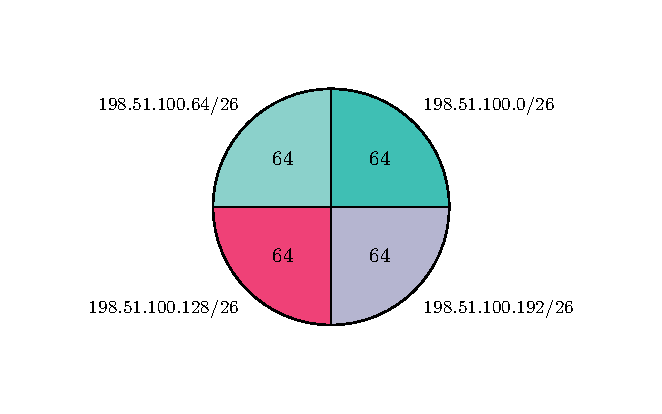
\includegraphics[width=\textwidth]{images/ip/subnetting.pdf}
\end{sidecaption}
\end{figure}

Let's start with the range 192.168.0.0/24.
The host part is eight bits in size so the range contains 256 \IP\ addresses.
Every time we add a bit to the network part, we split the range in two and thus half the number of available addresses per subnet.
If we change the prefix length to 25, we get two subnets each containing 128~addresses.
If we change the prefix length to 26, each of these two subnets gets halved again, all four parts containing 64~addresses.
When we make the prefix length 27~bits, we get eight subnets of 32~addresses each.

As you can see in \vref{fig:vlsm} you can take one subnet and divide it further into smaller parts.
In this case one of the four networks has been split again.
This is called \acf{VLSM}.

\begin{figure}
\begin{sidecaption}%
   [With \acs{VLSM} you can divide an \acs{IP} block in unequal parts]%
   {When using \acs{VLSM} you can further divide a subnet into smaller segments}%
   [fig:vlsm]
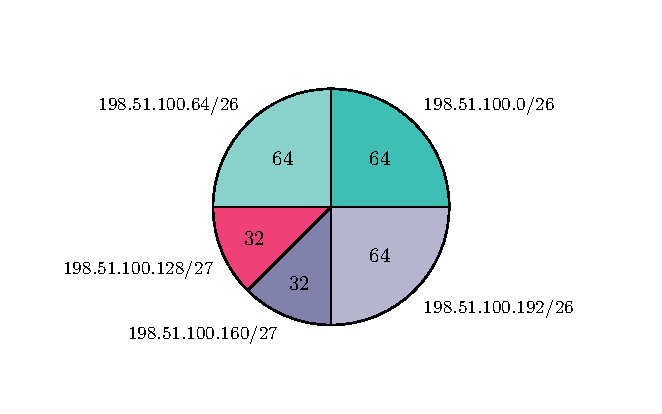
\includegraphics[width=\textwidth]{images/ip/vlsm.pdf}
\end{sidecaption}
\end{figure}


\paragraph{Why do we need subnetting?}
   \index{subnetting}
We are the network administrators of a small company.
We have a couple (50) of desktop computers for the employees, as well as a few (10) servers.
We contact \acs{RIPE} \acs{NCC}%
    \footnote{\gls{RIPE} \gls{NCC} is the \gls{RIR} for Europe, the Middle East and parts of central Asia. As a \gls{RIR}, it oversees the allocation and registration of internet number resources such as \acs{IP} addresses and autonomous system numbers.}
and tell them we need sixty \acs{IP} addresses, plus some extra just in case we will grow and need more computers.
Since a class~c address range contains 256~\acs{IP} addresses, \gls{RIPE} will give us one such range, e.g.~198.51.100.0/24.%
   \iacs{RIPE}

Now we have a problem.
We have plenty of \acs{IP} addresses but we need two separate networks.
Or perhaps we need three or even four.
Maybe we want to isolate the public internet-facing servers from the private servers that should not be reachable from the Internet.
We have received plenty of addresses, it is up to us to decide how to group them and to determine how large each network must be.

Remember that these different classes are just made-up methods of determining which part of the \acs{IP} address is the network number and which part is the host identifier.
\acs{IP} addresses themselves are just 32-bit numbers so we can group them any way we like.


\section{\acl{DHCP}}
\label{sec:ip-dhcp}


\paragraph{simplifies \acs{IP} address configuration}
   \iacs{DHCP}
Without the \gls{DHCP} you would have to contact a network administrator every morning at work when you power on your laptop and want to connect it to the (wireless) network.
Back at home or at a friend's place you need to change the \acs{IP} settings again, including which \acs{DNS} servers to use.
This requires huge lists with available \acs{IP} addresses which are being updated constantly with newly available \acs{IP} addresses -- should you remember to contact your network administrator before leaving work -- or available \acs{IP} addresses becoming unavailable as people come in to work every morning.%
   \footnote{%
      The first chapter of \textcite[3-7]{droms} gives a look in the life of a network administrator in the days when there was no \acs{DHCP} yet.
      I copied it to \vref{chap:dhcp-extract}.
   }

\paragraph{\acs{DORA}}
   \index{DHCP@\acs{DHCP}!DORA@\acs{DORA}}
\gls{DHCP} operations fall into four phases: server discovery, \acs{IP} address lease offer, lease request, and lease acknowledgement.
These stages (see \vref{fig:dora}) are often abbreviated as \acs{DORA} for \acl{DORA}.

\begin{figure}
\begin{sidecaption}{The foure stages of acquiring an \acs{IP} address from a \acs{DHCP} server}[fig:dora]
\centering
\tikzstyle{node}=[
    minimum width=20mm,
    minimum height=8mm,
    inner sep=0mm,
    font=\small\sffamily,
    text=black,
    node distance=12mm,
    draw=spot1,
    fill=spot1!20
]
\tikzstyle{arrow}=[->,>=stealth',semithick]

\begin{tikzpicture}

\node[node] (c) at (0,0) {client};
\node[node] (s) at (7,0) {server};

\draw [thick,arrow] (c) -- +(0,-4) node[below] {$t$};
\draw [thick,arrow] (s) -- +(0,-4) node[below] {$t$};

\node (start) at ($(c)-(0,1)$) {};

\draw [thick,arrow] (start.center) -- node[below] {\footnotesize discover} ++(7,-0.5);
\draw [thick,arrow,<-,spot2] ($(start)+(0,-1.2)$) -- node[below] {\footnotesize offer} ++(7,0.5);
\draw [thick,arrow] ($(start)+(0,-1.4)$) -- node[below] {\footnotesize request} ++(7,-0.5);
\draw [thick,arrow,<-,spot2] ($(start)+(0,-2.6)$) -- node[below] {\footnotesize acknowledge} ++(7,0.5);
\end{tikzpicture}
\end{sidecaption}
\end{figure}

\paragraph{lease time}
   \index{DHCP@\acs{DHCP}!lease time}
When the server offers the client an \acs{IP} address, it does this for a specific lease time.
After this time expires, the client must relinquish the given \acs{IP} address.
To prevent the client from getting disconnected from the network while it requests a new \acs{IP} address, it can refresh the lease on its current \acs{IP} address midway the lease period.

For example, when the client gets an \acs{IP} address with a lease time of eight hours, it can refresh the lease period after four hours.
If the server grants this request, the lease is again valid for eight hours.

If the \acs{DHCP} server denies the request, the client loses the lease right away.
It cannot use the \acs{IP} address for the remaining four hours but must send a \acs{DHCP} discover message to request a new \acs{IP} address.

\paragraph{\acs{DHCP} relay}
   \index{DHCP@\acs{DHCP}!relay}
As it is impractical to configure a \acs{DHCP} server on each network, routers can be configured to act as \acs{DHCP} relays, forwarding the broadcast messages%
   \fxwarning{Explain why \acs{DHCP} uses broadcast messages.}
as unicast to a remote \acs{DHCP} server.

\paragraph{reservations}
A \acs{DHCP} server can be configured such to always provide the same client (\acs{MAC} address) the same \acs{IP} address.
This way the client practically has a fixed \acs{IP} address, as if configured manually on the device itself.
But you keep the \acs{IP} address configuration on a central location.




\section{\Acl{NAT}}
\label{sec:ip-nat}


\paragraph{private \acs{IP} space}
There is nothing special about `private' \acs{IP} addresses.
   \index{IP address@\acs{IP} address!private}
   \index{IP address@\acs{IP} address!public}
   \index{internet}
   \iacs{ISP}
They are not treated any different from `public' \acs{IP} addresses by routers or end hosts.
The only difference is that they \emph{should} not be routed on the public internet.
This means that \acl{ISP} should block packets with a private \acs{IP} address as either the source or the destination address.

There are several blocks of private \acs{IP} addresses which can be used internally by organisations without having to ask for permission to do so.
\begin{multicols}{2}
\raggedcolumns
\begin{itemize}
\item 10.0.0.0/8
\item 100.64.0.0/10
\item 169.254.0.0/16
\item 172.16.0.0/12
\item 192.0.2.0/24
\item 192.168.0.0/16
\item 198.18.0.0/15
\item 198.51.100.0/24
\item 203.0.113.0/24
\end{itemize}
\end{multicols}

The ranges 10.0.0.0/8, 172.16.0.0/12, and 192.168.0.0/16 were introduced as private IP ranges to enable \acf{NAT}.
The ranges 192.0.2.0/24, 198.51.100.0/24, and 203.0.113.0/24 have been reserved for documentation purposes but can be used internally within an organisation.
The range 100.64.0.0/10 was added in 2012 for use in carrier-grade \ac{NAT} scenarios (\rfc{6598}):

\begin{quote}
Shared-address space is distinct from \rfc{1918} private address space because it is intended for use on service-provider networks.
However, it may be used in a manner similar to \rfc{1918} private-address space on routing equipment that is able to do address translation across router interfaces when the addresses are identical on two different interfaces.
\end{quote}

The address range 169.254.0.0/16 is a special case.
These are defined as `link-local' addresses and must not be forwarded by a router as these addresses are not guaranteed to be unique beyond their network segment.%
   \index{IP address@\acs{IP} address!link-local}
Microsoft names this range \acp{APIPA}.%
   \index{IP address@\acs{IP} address!APIPA@\acs{APIPA}}
A \acs{DHCP}\iacs{DHCP} client takes a random \acs{IP} address from this range when it receives no responses from any \acs{DHCP} server.

\paragraph{port-based address translation}
   \iacs{NAT}
The majority of network address translators map multiple private hosts to one publicly exposed \acs{IP} address.
In a typical configuration, a local network uses one of the designated private \acs{IP} address subnets (\rfc{1918}).
One or more routers sit at the border of this private network connecting it to the public Internet.

As traffic passes from the local network to the Internet, the source address in each packet is translated on the fly from its private address to the public address of the router.
The router tracks basic metadata about each active connection (particularly the destination address and port).
When a reply returns to the router, it uses the connection tracking data it stored during the outbound phase to determine the private address on the internal network to which to forward the reply.

All \acs{IP} packets have a source \acs{IP} address and a destination \acs{IP} address.
Typically packets passing from the private network to the public network will have their source address modified, while packets passing from the public network back to the private network will have their destination address modified.
To avoid ambiguity in how replies are translated, further modifications to the packets are required.
For \acs{TCP} and \acs{UDP} the port numbers are changed so that the combination of \acs{IP} address and port number on the returned packet can be unambiguously mapped to the corresponding private network destination.
\rfc{2663} uses the term \gls{NAPT} for this type of \acs{NAT}.
Other names include \gls{PAT}, \acs{IP} \emph{masquerading}, \acs{NAT} \emph{overload} and \emph{many-to-one} \acs{NAT}.
This is the most common type of \acs{NAT} and has become synonymous with the term \acs{NAT} in common usage.
   \index{IP masquerading@\acs{IP} masquerading}
   \index{NAT@\acs{NAT}!overload}
   \index{NAT@\acs{NAT}!many-to-one}
   \iacs{PAT}

\paragraph{pool of public addresses}
   \index{NAT@\acs{NAT}!pool}
It is possible to use multiple public \acs{IP} addresses to translate the private \acs{IP} address into.
When this is used in combination with port-based address translation, it allows for multiple thousands of private hosts to communicate on the Internet.

% TODO: either explain more, or delete?
\extrap{one-to-one translation}
   \index{NAT@\acs{NAT}!static}
   \index{NAT@\acs{NAT}!one-to-one}
This method is most often used to translate a range of private \acs{IP} addresses into a different range of private \acs{IP} addresses.
This is often needed when two companies with overlapping \acs{IP} address space connect their networks together.






\section{\acs{IP} header}
Before we delve into the second major topic, \IP\ routing, let's first take a look at the \IPfour\ packet header.

\begin{figure}
\begin{sidecaption}{The \IPfour\ packet header}[fig:ipv4-header]
\centering
\begin{bytefield}{32}
\bitheader{0,3,4,7,8,13-15,16,18,19,31}\\
\bitbox{4}{version}
\bitbox{4}{\SC{IHL}}
\bitbox{6}{\SC{DSCP}}
\bitbox{2}{\footnotesize\SC{ECN}}
\bitbox{16}{total length} \\
\bitbox{16}{identification}
\bitbox{3}{flags}
\bitbox{13}{fragment offset} \\
\bitbox{8}{\acs{TTL}}
\bitbox{8}{protocol}
\bitbox{16}{checksum} \\
\wordbox{1}{source \IP\ address} \\
\wordbox{1}{destination \IP\ address} \\
\wordbox[tlr]{1}{options}\\
\skippedwords \\
\wordbox[blr]{1}{}\\
\end{bytefield}
\end{sidecaption}
\end{figure}

Most fields are not important to us but a few are.
\begin{description}
\item[source \IP\ address]
   The \IP\ address of the end host sending the packet.
\item[destination \IP\ address]
   The \IP\ address of the end host to which we want to send the packet.
\item[\acf{TTL}]
   The source puts a value (0-255) in this 8-bit field and every router forwarding the packet first decrements this value by one.
   When the number reaches zero, the packet is discarded.
   This is a simple method to prevent loops in the network where packets travel endlessly in a circle between two or more routers.
\item[protocol]
   The value in this 8-bit determines the contents of the packet.
   This value tells the operating system receiving the packet from the network to which higher-level protocol to send the data.
\item[checksum]
   A checksum of the header is calculated and stored in this field.
   The receiver calculates the checksums and compares it to this value.
   If both values are the same, the receiver can assume the data to be correct.
   If both checksums differ, the packet has been corrupted in transit and is discarded.
\end{description}

\begin{margintable}
\begin{tabular}{rl}
 1 & \acs{ICMP}  \\
 6 & \acs{TCP}   \\
17 & \acs{UDP}   \\
47 & \acs{GRE}   \\
50 & \acs{ESP}   \\
51 & \acs{AH}    \\
88 & \acs{EIGRP} \\
89 & \acs{OSPF}  \\
\end{tabular}
\caption{A few important \IP\ protocol values.}
\end{margintable}

\IPfour\ options are not often used and some can even be dangerous.
Many networks are configured to drop packets with either the \emph{Loose source and record route} option or the \emph{Strict source and record route} option.

In \IPsix\ options are implemented as extensions.
For example the IPsec \acf{AH} and \acf{ESP} headers are implemented as \IPsix\ extension headers.
   \index{VPN@\acs{VPN}!IPsec}
Fragmentation is also implemented using an extension header although \IPsix\ packets are not supposed to be fragmented.





\section{\Acl{ICMP}}
\label{sec:ip-icmp}

The \acf{ICMP} is a supporting protocol in the internet protocol suite.
It is used by network devices, including routers, to send error messages and operational information indicating success or failure when communicating with another \acs{IP} address, for example, an error is indicated when a requested service is not available or that a host or router could not be reached.

The program \cmd{ping} uses \acs{ICMP} to detect whether the destination is reachable and alive.
It sends out an \acs{ICMP} echo request (\cref{tab:icmp}) and expects to receive an \acs{ICMP} echo reply from the destination.
Receiving this reply tells us two things:
\begin{itemize}
\item
   the destination host is turned on and connected to the network as it was able to receive our message and reply to it;
\item
   the network between our computer and the destination is working as all the devices in the middle were able to send our request to the destination as well as send its reply back to us.
\end{itemize}

\begin{table}
\begin{sidecaption}{Most common \acs{ICMP} types and codes}[tab:icmp]
\centering
\begin{tabular}{rrl}
{type} & {code} & {description} \\
\midrule
 0 &  0 & echo reply \\
 3 &  0 & destination network unreachable \\
 3 &  1 & destination host unreachable \\
 3 &  2 & destination protocol unreachable \\
 3 &  3 & destination port unreachable \\
 3 &  4 & fragmentation needed but \SC{DF}-bit set \\
 3 & 13 & communication administratively prohibited \\
 5 &  0 & redirect datagram for the network \\
 5 &  1 & redirect datagram for the host \\
 8 &  0 & echo request \\
11 &  0 & \acs{TTL} expired in transit \\
\end{tabular}
\end{sidecaption}
\end{table}

If we do not receive a reply from the end host it can be because of one or more issue in the network.
\begin{itemize}
\item
   The end host could be turned off, have a firewall configured which prohibits sending or receiving \acs{ICMP} messages, or have an incorrect gateway configured so that the reply cannot reach us.
\item
   A network firewall in the path between source and destination can prevent the \acs{ICMP} query from reaching the destination.
   It could also prevent the reply form reaching us.
\item
   The destination network could be unknown to one of the routers in the path preventing the query from reaching its destination.
   Our own network could also be unknown to one of the routers in the path preventing the reply from reaching us.
\end{itemize}
More troubleshooting is needed to determine the exact problem or problems so that they can get fixed.
A good place to start would be to use the program \cmd{traceroute} (on Windows it is called \cmd{tracert}).

\fxwarning{Complete this section.}


\paragraph{\acl{PMTUD}}

\Acf{PMTUD} is a standardized technique in computer networking for determining the \acf{MTU} size on the network path between two \IP\ hosts, usually with the goal of avoiding \IP\ fragmentation.
\Acl{PMTUD} was originally intended for routers in \IP\ version~4.
However, all modern operating systems use it on endpoints.

\Acl{PMTUD} works by setting the \emph{don't fragment} (\SC{DF}) flag bit in the \IP\ headers of outgoing packets.
Then, any device along the path whose \acs{MTU} is smaller than the packet will drop it, and send back an \acs{ICMP} \emph{fragmentation needed} (type~3, code~4) message containing its \acs{MTU}, allowing the source host to reduce its path \acs{MTU} appropriately.
The process is repeated until the \acs{MTU} is small enough to traverse the entire path without fragmentation.

See also \emph{time-to-live} on p.~\pageref{par:ip-ttl} and \emph{fragmentation} on p.~\pageref{par:ip-fragmentation}.







\section{Routing}
\label{sec:ip-routing}

\paragraph{What is a router?}
   \index{router}
   \index{packet!forwarding}
A router is really just a specialised computer that \emph{forwards} packets it receives but which are not destined for itself.
A computer can also be configured to function as a router by turning on this option (\vref{lst:freebsd-enable-routing,lst:rhel-enable-routing}).


\begin{fltlisting}[h!]
\begin{sidecaption}{Enable routing on a FreeBSD host}[lst:freebsd-enable-routing]
\begin{lstlisting}
# sysrc gateway_enable="YES"
# sysctl net.inet.ip.forwarding=1
\end{lstlisting}
\end{sidecaption}
\end{fltlisting}

\begin{fltlisting}[h!]
\begin{sidecaption}{Enable routing on a \acs{RHEL} host}[lst:rhel-enable-routing]
\begin{lstlisting}
# echo "net.ipv44.ip_forward=1" >> /etc/sysctl.conf
# echo 1 > /proc/sys/net/ipv4/ip_forward
\end{lstlisting}
\end{sidecaption}
\end{fltlisting}

\fxwarning{These new listings don't play nice with \textbackslash{}vref.}

When a router receives a packet with a destination \acs{IP} address which does not belong to any of the router's interfaces, the router looks up the \acs{IP} address in its \emph{routing table} and forwards the packet out the given interface.%
   \index{routing table}

\begin{fltlisting}[h!]
\begin{sidecaption}{The routing table on a linux machine}[fig:routing-table]
\begin{lstlisting}
[doyle] ~ $ netstat -rn
Kernel IP routing table
Destination     Gateway         Genmask         Iface
10.0.0.0        172.24.12.1     255.255.240.0   eth1
10.0.16.0       172.24.12.1     255.255.240.0   eth1
10.0.32.0       192.168.16.1    255.255.224.0   eth2
172.21.3.0      0.0.0.0         255.255.255.0   eth0
172.24.12.0     0.0.0.0         255.255.255.0   eth1
192.168.16.0    0.0.0.0         255.255.255.0   eth2
0.0.0.0         172.21.3.1      0.0.0.0         eth0
\end{lstlisting}
\end{sidecaption}
\end{fltlisting}

Routers only know about the networks they directly connect to.
They must thus learn about distant networks.
This can happen in one of two ways, either the network administrator manually configures the router to forward a certain prefix to some other router (the \emph{next-hop} router) or the routers in a network can use a \emph{dynamic routing protocol} to teach each other about the networks they know and how to reach them.
   \index{router!next-hop}

\begin{marginfigure}
\noindent
\fxwarning[layout=inline]{Insert a figure here.}
\caption{Router $R_1$ knows about networks~1 and~2, but not about network~3.}
\label{fig:ip-local-networks}
\end{marginfigure}

\paragraph{\acl{TTL}}
\label{par:ip-ttl}
   \iacs{TTL}
The \acs{IP} header contains a \gls{TTL} field which indicates how many routers (hops) it can pass before it must be deleted.
This prevents the data packet from circulating indefinitely.
As it is an 8-bit field, the maximum value is~255 but a recommended initial value is~64.\footnote{See \rfc{1700}, p.~64.}

As it does not really signify some time spent in transit, with the development of \acs{IP} version~6, they changed the name of this field to \emph{hop limit} as that is what it really does: limit the number of hops (routers) that a packet can travel.


\paragraph{fragmentation}
\label{par:ip-fragmentation}
   \index{fragmentation}
   \iacs{MTU}
Different physical media have different maximum frame sizes.
For example, Ethernet has a maximum frame size of 1518~bytes or a \gls{MTU} of 1500~bytes, which is the frame size minus the header length.
Token Ring has a much larger \gls{MTU} of 4464~bytes, \gls{ATM} and \SC{X.25} have much smaller \acp{MTU} of 48~and 576~bytes respectively.

When a router connects an Ethernet segment to an \gls{ATM} circuit, it must \emph{fragment} the 1500-byte frames it receives into 48-byte cells that it can forward across the \ac{ATM} network.
Once fragmented, routers do not reassemble the pieces back together as they might take different paths through the network and are not guaranteed to arrive in the correct order.
The end host is responsible for piecing all fragments back together.

Another example when fragmentation is being used, is in the communication between a data centre and campus network as the former often uses jumbo frames (an \acs{MTU} of 9000~bytes) while the latter uses normal Ethernet frames which have an \acs{MTU} of 1500~bytes.%
   \index{frame!jumbo}
   \index{data centre}

Finally, you will also encounter fragmentation on IPsec \aclp{VPN} where the maximum transmission unit is slightly smaller than the normal 1500~bytes.
   \index{VPN@\acs{VPN}!IPsec!fragmentation}

\paragraph{broadcast domain}
   \index{broadcast domain}
A \emph{broadcast domain} is that part of the network to which a broadcast messages propagates.
One of the functions of a router is to stop broadcasts, not forwarding the to other parts of the network.

\paragraph{static routing}
   \index{static routing}
Static routing is a form of routing that occurs when a router uses a manually-configured routing entry, rather than information from dynamic routing traffic.
In many cases, static routes are manually configured by a network administrator by adding in entries into a routing table, though this may not always be the case.
Unlike dynamic routing, static routes are fixed and do not change if the network is changed or reconfigured.
Static routing and dynamic routing are not mutually exclusive.
Both dynamic routing and static routing are usually used on a router to maximise routing efficiency and to provide backups in case dynamic routing information fails to be exchanged.
Static routing can also be used in \emph{stub networks},%
\index{stub network}%
\footnote{%
A stub network is a (part of a) network with only one way to reach the rest of the network.
It thus does not need detailed knowledge about the network but can usually route all traffic using a single default route pointing to the exit point.
}
or to provide a gateway of last resort.

\pagebreak
\paragraph{dynamic routing protocols}%
   \index{routing protocol!distance-vector}%
   \index{routing protocol!link-state}%
\begin{description}
\item[distance-vector]
A distance-vector routing protocol is like putting signposts on every crossroads with the router being the crossroads.
Every router learns about all networks but only the direction it has to send traffic to (the next-hop router) and the total distance to reach the remote network.
\item[link-state]
A link-state routing protocol is comparable to every router building a roadmap with all links interconnecting the different routers included.
Once the entire map has been drawn, each router can calculate the best path to reach each destination.
\end{description}

\paragraph{metric}
   \index{metric}
When we take a look at \vref{fig:metric}, we see that router $R_4$ connects to the network 192.0.2.0/24.
It advertises this to routers $R_2$ and $R_3$ which in turn both advertise this network to router $R_1$.
Router $R_1$ now knows two paths to reach the destination network 192.0.2.0/24, once via $R_2$ and once via $R_3$.
For $R_1$ to decide which path is best, it compares the \emph{metric} of both paths; the lowest value is the best path.

When a router advertises a network, it includes a metric value.
When another router forwards this information -- e.g.~router $R_2$ forwards the information about network 192.0.2.0/24 to router $R_1$ -- it updates the metric value.

Every routing protocol can use a different metric.
\acs{RIP} uses a simple \emph{hop count} or the number of routers you have to traverse to reach your destination.
\acs{OSPF} and \acs{IS-IS} use a generic \emph{cost} value.
Most \acs{OSPF} implementation use a cost value based on the bandwidth of the links while with \acs{IS-IS} the network administrator has to manually set a cot value for each link.
\acs{EIGRP} uses a very complex formula to determine the metric, see \vref{eqn:eigrp-metric}.

\begin{figure}
\begin{sidecaption}[The metric decides the best route in a network]{A router can learn a prefix from several other routers. The metric decides the best route.}[fig:metric]
\centering
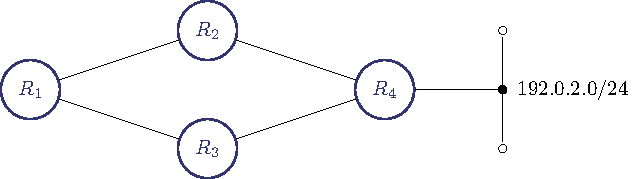
\includegraphics[width=\textwidth]{images/ip/metric.pdf}
\end{sidecaption}
\end{figure}


\paragraph{equal-cost multi-path routing}
   \iacs{ECMP}
   \index{load balancing!network}
If both $R_2$ and $R_3$ advertise the same metric towards $R_1$ both paths are equally good and $R_1$ \emph{load balances} traffic over both paths.
The router uses an algorithm to send roughly fifty percent of packets via $R_2$ and the other fifty percent via~$R_3$.

\paragraph{administrative distance}
   \index{administrative distance}
The \emph{metric} indicates the preference of a single route learnt from different routers via the same routing protocol.
It is however also possible for a router to learn a route from different routing protocols.
The \emph{administrative distance} gives the preference or credibility of a routing protocol over another.
For example, on Cisco routers the administrative distance or credibility of \acs{RIP} is~110 while the administrative distance of \acs{OSPF} is~90.
As lower values are preferred, when a router running both \acs{RIP} and \acs{OSPF} learn about the same route from both protocols, it will prefer the route learnt from \acs{OSPF} over the route learnt from \acs{RIP}.%
   \footnote{%
      The administrative distance is -- as the name implies -- a purely administrative value, meaning the network administrator chooses which routing protocol to prefer over the other.
      However, as a best practice a network should only use a single routing protocol.
      It is not good to combine several routing protocols as the network then becomes needlessly complex and error prone.
   }

\paragraph{\acf{RIP}}
The \acl{RIP} is an example of a distance-vector routing protocol using the \emph{hop count} or the number of routers to count how good a given path is.%
   \index{metric!hop count}
It is a very simple protocol useful in smaller networks.
The protocol is not suitable for larger networks because of its slow \emph{convergence time} and its tendency to propagate good information slowly and negative information quickly.
   \index{convergence time}

\extrap{route poisoning}
   \index{route poisoning}
% source: https://www.geeksforgeeks.org/route-poisoning-and-count-to-infinity-problem-in-routing/
The main issue with distance-vector routing protocols is routing loops.%
   \fxwarning{Briefly explain routing loops.}
   \index{routing loop}
This routing loop in the network causes the count-to-infinity problem.%
   \fxwarning{Briefly explain the count-to-infinity problem.}
   \index{count-to-infinity}
Routing loops usually occur when an interface goes down or two routers send updates at the same time.

Route poisoning helps to alleviate this problem by advertising the route back to its source with a metric of infinity.
This ensures that the router originally advertising the prefix can never use its neighbours to reach the given network.

\extrap{split horizon}
   \index{split horizon}
Split horizon is another method to prevent routing loops from occuring.%
   \index{routing loop}
This time, instead of advertising the routes back with a metric of infinity, we simple do not advertise the route back to where we learned it from.
This method is not as good as using route poisoning to prevent routing loops.
Logically you can not use both both methods. Either you use neither method, or you use one or the other.

\extrap{hold-down timer}
   \index{hold-down timer}
When a router receives a routing update advertising a network to be unreachable, it starts a hold-down timer.
Until the timer expires, the router will discard any subsequent route messages that indicate the route is in fact reachable.
It can solve the case where multiple routers are connected indirectly.
There are realistic scenarios where split horizon and split horizon with poisoned reverse can do nothing.%
\fxwarning{This is very vague.}

\paragraph{\acl{EIGRP}}
   \iacs{EIGRP}
The \acf{EIGRP} was a Cisco proprietary protocol which has been made publicly available in 2013 but has not been implemented by other vendors.

While \acs{RIP} and \acs{OSPF} have a very simple metric, \acs{EIGRP} has a rather complex one.
The metric $m$ is calculated as such:
\begin{equation}
m = \left[\left(k_1 B_m  + k_2 \frac{B_m}{256-L} + k_3 D_s\right) \times \frac{k_5}{k_4 + R}\right] \times 256,
\label{eqn:eigrp-metric}
\end{equation}
with $B_m$ being the minimum bandwidth along the path to the destination, $D_s$ being the total delay along the path, $L$ and $R$ being the load an the reliability of the link respectively, taken over a five-minute interval.
The five $k$ values are user-configurable weights to each part of the equation.%
   \footnote{%
      My advice is to change these $k$ values to exclude the bandwidth from the equation.
      Altering the bandwidth value also changes the calculations for \acs{QOS} among other things while the delay value is used only by \acs{EIGRP}.
      This will result in more readable metrics and it will be easier to tune \acs{EIGRP} without interfering with other services on the router.
      See the exercises on how to do this.
   }

As if \cref{eqn:eigrp-metric} is not complex enough, there are a few important caveats.
The minimum bandwidth $B_m$ is calculated by dividing a reference bandwidth of \SI{1e7}{\bit\per\second} by the smallest configured bandwidth on the interfaces along the path.
It does not take into account the actual bandwidth of an interface, but the setting configured on the interface.

The total delay also is not measured along the path but fixed values are used depending on the interface type.
A serial interface always has a default delay of \SI{20000}{\micro\second} while a Gigabit Ethernet interface has a default delay of \SI{10}{\micro\second}, regardless of the length of the cable.
Both settings are user configurable.
The value $D_s$ is measured in tens of microseconds so for a serial interface the value 2000 would be used instead of \numprint{20000}.

\begin{margintable}
\begin{tabular}{lr}
serial   & {20000} \\
\SC{T1}  & {20000} \\
Ethernet & 1000  \\
FastE    & 100   \\
GigE     & 10    \\
10GigE   & 10    \\
\end{tabular}
\caption{Default delay values per interface type}
\label{tab:ip-intf-delay}
\end{margintable}

If load an reliability are used in the computation -- which by default they are not -- the initial values are set during peer establishment and do not change dynamically with the router.
These values are a remnant of an older version of the protocol where they did change with every update to reflect the live status of the network.

Finally, when $k_5=0$, instead of the entire equation to become zero, this factor is removed from the equation.

\paragraph{\acf{OSPF}}
   \iacs{OSPF}
The \acl{OSPF} protocol is a link-state routing protocol suitable for small network all the way up to massive service provider networks.
It can scale to very large networks because of the introduction of a concept called \emph{areas}, used to divide the entire network into smaller, more manageable parts.

The \acs{OSPF} metric $m$ is calculated by summing all costs along the path with the cost being a reference bandwidth devided by the actual bandwidth $B_i$ of the link.

\begin{margintable}
\begin{tabular}{lr}
\SC{T1}  & 64      \\
Ethernet & 10      \\
FastE    & 1       \\
GigE     & 1       \\
10GigE   & 1       \\
\end{tabular}
\caption{Default \acs{OSPF} cost values per interface type}
\label{tab:ip-ospf-cost}
\end{margintable}

\begin{equation}
m = \sum_i\frac{10^8}{B_i}
\end{equation}

As you can see in \vref{tab:ip-ospf-cost} \acs{OSPF} by default cannot differentiate between a FastEthernet link at \SI{100}{\mega\bit\per\second} or a 10GigE link, while it clearly should!
Thus it is very important that you change the refence bandwidth on \emph{all} your routers in the network to a value higher than your highest network link (see the practice questions).


\paragraph{\acf{BGP}}
   \iacs{BGP}
   \index{routing protocol!path-vector}
   \index{autonomous system}
The \acl{BGP} is neither a distance-vector nor a link-state routing protocol.
It is the only \emph{path-vector} routing protocol and it is used to interconnect different \emph{autonomous systems}, meaning it can be used to interconnect networks operated by different organisations.
A basic \acs{BGP} configuration is relatively simple but it can quickly become extremely complex.

Contrary to normal routing protocols which serve to make all networks known within the entire internetwork, \acs{BGP} aims to limit reachability and focusses on \emph{policies}.
You can tweak the protocol so that you can exactly control the path a packet has to travel through the network to reach its destination.



\section{Review questions}
\label{sec:ip-review-questions}
\fxwarning{I should probably differentiate between review questions for the theory course, guided exercises for the extra hands-on course and practice questions for students to do at home.}

\begin{enumerate}
\item
   Given the network 100.65.0.0/16, give the network address, broadcast address, and the first and last available \IP\ addresses.
\item
   Given the network 198.19.0.0/24, give the network address, broadcast address, and the first and last available \IP\ addresses.
\item
   Given the network 203.0.113.32/27, give the network address, broadcast address, and the first and last available \IP\ addresses.
\item
   How many available or usable \IP\ addresses are there in the network 192.168.12.128/25?
\item
   Which class of \IP\ addresses provides a maximum of only 254 host addresses per network \SC{ID}?
   \begin{multicols}{2}
   \raggedcolumns
   \begin{enumerate}
   \item class a
   \item class b
   \item class c
   \item class d
   \item class e
   \end{enumerate}
   \end{multicols}
\item
   Given the \IP\ range 192.0.2.64/26, split this range up into four smaller blocks.
   Give the network and broadcast address for each of these four subnetworks.
\item
   What is the maximum number of \IP\ addresses that can be assigned to hosts on a local subnet that uses the 255.255.255.224 subnet mask?
   \begin{multicols}{2}
   \begin{enumerate}
   \item 14
   \item 15
   \item 16
   \item 30
   \item 31
   \item 62
   \end{enumerate}
   \end{multicols}
\item
   What is the subnetwork address for a host with the \IP\ address 200.10.5.68/28?
   \begin{multicols}{2}
   \begin{enumerate}
   \item 200.10.5.56
   \item 200.10.5.32
   \item 200.10.5.64
   \item 200.10.5.0
   \end{enumerate}
   \end{multicols}
\item
   You want to implement a mechanism that automates the \IP\ configuration, including \IP\ address, subnet mask, default gateway, and \acs{DNS} information.
   Which protocol will you use to accomplish this?
   \begin{multicols}{2}
   \begin{enumerate}
   \item \acs{SMTP}
   \item \acs{ARP}
   \item \acs{DHCP}
   \item \acs{SNMP}
   \end{enumerate}
   \end{multicols}
\item
   You have an interfaces on a router with the \IP\ address of 192.168.192.10/29.
   What is the broadcast address the hosts will use on this \acs{LAN}?
   \begin{multicols}{2}
   \begin{enumerate}
   \item 192.168.192.15
   \item 192.168.192.31
   \item 192.168.192.63
   \item 192.168.192.127
   \item 192.168.192.255
   \item 192.168.255.255
   \end{enumerate}
   \end{multicols}
\item
   To test the \IP\ stack on your local host, which \IP\ address would you ping?
   \begin{multicols}{2}
   \raggedcolumns
   \begin{enumerate}
   \item 127.0.0.0
   \item 1.0.0.127
   \item 127.0.0.1
   \item 127.0.0.255
   \item 255.255.255.255
   \end{enumerate}
   \end{multicols}
\item
   Which two of the following are private \IP\ addresses?
   \begin{multicols}{2}
   \begin{enumerate}
   \item 25.7.0.1
   \item 172.33.194.4
   \item 169.172.19.93
   \item 172.19.25.54
   \item 192.168.77.12
   \item 203.0.113.7
   \end{enumerate}
\end{multicols}
\end{enumerate}

\section{Guided exercises}
\label{sec:ip-guided-exercises}

\section{Practice questions}
\label{sec:ip-practice-questions}
\begin{enumerate}
\item
   Create a small network with a router, a switch and two computers.
   Configure the router's interface with the \IP\ address 192.168.0.1/26 and configure a \acs{DHCP} server so that the computers automatically get an \IP\ address when they power on.
   One computer should always get the \IP\ address 192.168.0.7.
\item
   Set up a small network with a few routers and configure \acs{EIGRP} as the routing protocol between them.
\item
   Change the $k$ values so that only the interface delay is used to calculate the metric.
\item
   Set up a small network with a few routers and configure \acs{OSPF} as the routing protocol between them.
\item   
\label{ex:ip-ospf-ref-bw}
   Change the reference bandwidth for \acs{OSPF} to match \SI{100}{\giga\bit\per\second}.
\end{enumerate}



\section{Further reading}
\label{sec:ip-reading}
\textcite{lammle-ccna,lammle-comptia} are both good resources to continue from here.
They both explain \acs{IP} addresses, subnetting, \acs{DHCP}, and routing in more detail.
Another great resource is \textcite{stevens} but this masterpiece is probably a bit too in-depth.
\textcite{doyle} is another classic.
The first volume focusses on the routing protocols \acs{RIP}, \acs{OSPF}, and \acs{IS-IS} while the second volume covers \acs{BGP}.
\Chapter{Transport layer protocols}
\label{chap:transport-layer}

\Section{\acl{UDP}}
\label{sec:udp}

\Paragraph{port numbers}
\mode<article>{
In computer networking, a port is a communication endpoint.
At the software level, within an operating system, a port is a logical construct that identifies a specific process or a type of network service.
A port is identified for each transport protocol and address combination by a 16-bit unsigned number, known as the \emph{port number}.

A port number is always associated with an \acs{IP} address of a host and the type of transport protocol used for communication.
It completes the destination or origination network address of a message.
Specific port numbers are reserved to identify specific services so that an arriving packet can be easily forwarded to a running application.
For this purpose, port numbers lower than 1024 identify the historically most commonly used services and are called the \emph{well-known port numbers}.
Higher-numbered ports are available for general use by applications and are known as \emph{ephemeral ports}.

\Vref{tab:port-numbers} lists a few well-known port numbers while \vref{tab:ephemeral-ports} lists the range of port numbers used by some operating systems.

\begin{table}
    \centering
    \sffamily
    \begin{tabular}{rl}
    \textbf{port} & \textbf{application} \\[1ex]
     22 & \acs{SSH} \\
     25 & \acs{SMTP} \\
     53 & \acs{DNS} \\
     67 & \acs{DHCP} (server) \\
     68 & \acs{DHCP} (client) \\
     80 & HTTP \\
    110 & POP3 \\
    143 & IMAP \\
    443 & HTTPS \\
    \end{tabular}
    \caption{A few well-known ports}
    \label{tab:port-numbers}
\end{table}

\begin{table}
    \centering
    \sffamily
    \begin{tabular}{lr@{--}l}
    \textbf{operating system} & \multicolumn{2}{l}{\textbf{port range}} \\[1ex]
    Many Linux kernels & \num{32768} & \num{60999} \\
    FreeBSD            & \num{49152} & \num{65535} \\
    Windows XP         & \num{1025} & \num{5000} \\
    Windows 7          & \num{49152} & \num{65535} \\
    \end{tabular}
    \caption{Port ranges used by operating systems as ephemeral ports}
    \label{tab:ephemeral-ports}
\end{table}
}
\slide{well-known port numbers}
\slide{ephemeral port numbers}


\Paragraph{checksum}
\mode<article>{
A checksum is a small-sized block of data derived from another block of digital data for the purpose of detecting errors that may have been introduced during its transmission or storage.
By themselves, checksums are often used to verify data integrity but are not relied upon to verify data authenticity.
}

\Paragraph{`unreliable'}
\mode<article>{
The \ac{UDP} does not keep track of which packets have been sent and received correctly.
It sends data and forgets about it.
Should the application require reliability, it itself is responsible for this function.
This lack of reliability makes \ac{UDP} a very fast protocol.
}

\Section{\acl{TCP}}
\label{sec:tcp}


\Paragraph{port numbers and checksum}
\mode<article>{
See \cref{sec:udp}.
}

\Paragraph{`reliable'}
\mode<article>{
The \ac{TCP} makes sure all data that is sent, is also received correctly by the destination.
It uses a combination of \emph{sequence numbers} and \emph{acknowledgements} to achieve this reliability.
}

\Paragraph{three-way handshake}
\mode<article>{
Before a client attempts to connect with a server, the server must first bind to and listen at a port to open it up for connections: this is called a passive open.
Once the passive open is established, a client may establish a connection by initiating an active open using the three-way handshake.
\begin{description}
\item[\abbr{SYN}]
The active open is performed by the client sending a \abbr{SYN} to the server.
The client sets the segment's sequence number to a random value $A$.
\item[\abbr{SYN+ACK}]
In response, the server replies with a \abbr{SYN+ACK}.
The acknowledgement number is set to one more than the received sequence number i.e. $A+1$, and the sequence number that the server chooses for the packet is another random number, $B$.
\item[\abbr{ACK}]
Finally, the client sends an \abbr{ACK} back to the server.
The sequence number is set to the received acknowledgment value i.e. $A+1$, and the acknowledgment number is set to one more than the received sequence number i.e. $B+1$.
\end{description}
Steps 1 and 2 establish and acknowledge the sequence number for one direction.
Steps~2 and~3 establish and acknowledge the sequence number for the other direction.
Following the completion of these steps, both the client and server have received acknowledgements and a full-duplex communication is established.
}

\Paragraph{acknowledgements}
\mode<article>{
\ac{TCP} uses a sequence number to identify each byte of data.
The sequence number identifies the order of the bytes sent from each computer so that the data can be reconstructed in order, regardless of any out-of-order delivery that may occur.
The sequence number of the first byte is chosen by the transmitter for the first packet, which is flagged \abbr{SYN}.
This number can be arbitrary, and should, in fact, be unpredictable to defend against \ac{TCP} sequence prediction attacks.

Acknowledgements (\abbr{ACK}) are sent with a sequence number by the receiver of data to tell the sender that data has been received to the specified byte.
Acknowledgements do not imply that the data has been delivered to the application, they merely signify that it is now the receiver's responsibility to deliver the data.

Reliability is achieved by the sender detecting lost data and retransmitting it.
\ac{TCP} uses two primary techniques to identify loss: retransmission timeout (\abbr{RTO}) and duplicate cumulative acknowledgements.
}

\Paragraph{flow control}
\mode<article>{
\acs{TCP} uses a \emph{sliding window} flow control protocol.
In each \acs{TCP} segment, the receiver specifies in the \emph{receive window} field the amount of additionally received data (in bytes) that it is willing to buffer for the connection.
The sending host can send only up to that amount of data before it must wait for an acknowledgement and receive window update from the receiving host.
}

\Paragraph{congestion control}
\mode<article>{
The final main aspect of \acs{TCP} is congestion control.
\acs{TCP} uses a number of mechanisms to achieve high performance and avoid congestion collapse, where network performance can fall by several orders of magnitude.
These mechanisms control the rate of data entering the network, keeping the data flow below a rate that would trigger collapse.
They also yield an approximately max-min fair allocation between flows.

Acknowledgments for data sent, or lack of acknowledgments, are used by senders to infer network conditions between the \acs{TCP} sender and receiver.
Coupled with timers, \acs{TCP} senders and receivers can alter the behavior of the flow of data.
This is more generally referred to as \emph{congestion control} and/or \emph{network congestion avoidance}.

Modern implementations of \acs{TCP} contain four intertwined algorithms: \emph{slow-start}, congestion avoidance, \emph{fast retransmit}, and \emph{fast recovery} (\acs{RFC}~5681).
}
\chapter{Ethernet}
\label{sec:ethernet}

In \vref{sec:arp} hadden we gezien hoe een computer het destination MAC-adres bekomt als hij een frame wilt versturen over het netwerk.
In dit hoofdstuk leren we hoe switches deze frames naar hun bestemming sturen en welke gevaren er schuil gaan in een netwerk op laag~2.

\subsection{De werking van Ethernet}


\begin{figure}[hbp]
    \centering
    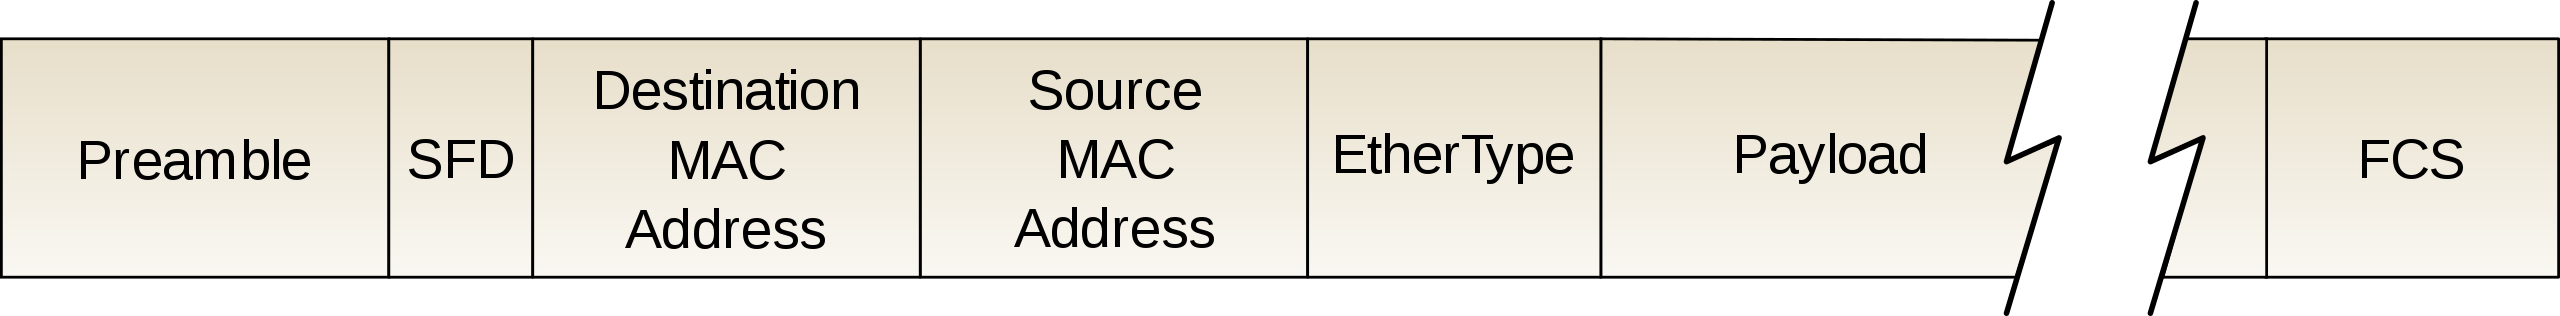
\includegraphics[width=\textwidth]{images/Ethernet_frame.png}
    \caption{An Ethernet frame inside an Ethernet packet, with SFD marking the end of the packet preamble and indicating the beginning of the frame}
    \label{fig:ethernet-frame}
\end{figure}


\Vref{fig:ethernet-frame} toont de velden in een Ethernet frame.
Eerst komen de \emph{preamble} en de \emph{start of frame delimiter} (SFD).
Deze dienen om het kloksignaal van de ontvanger af te stemmen op het kloksignaal van de zender zodat beide machines weten hoe lang het signaal van een 0 of een 1 duurt.

Hierna begint het eigenlijke Ethernet frame met het destination MAC-adres, gevolgd door het MAC-adres van de zender.
De \emph{EtherType} vertelt de ontvanger wat voor data er wordt verstuurd.
Enkele voorbeelden van geldige EtherTypes worden gegeven in \vref{tab:ethertype}.
Hierna komt de eigenlijke data of de \emph{payload} en ten slotte komt de \emph{frame check sequence} (FCS).
Dit is een code die gebruikt wordt om te detecteren of er fouten in het frame zitten.
Als het frame corrupt is, wordt deze gewoon verwijderd.
De ontvanger verwittigt de zender van het frame niet dat het frame niet goed is aangekomen.

\begin{table}[htp]
    \centering
    \begin{tabular}{ll}
    \textit{EtherType} & \textit{protocol} \\[1ex]
    0x0800 & IPv4 \\
    0x0806 & address resolution protocol (ARP) \\
    0x8100 & VLAN-tagged frame \\
    0x86DD & IPv6 \\
    \end{tabular}
    \caption{Enkele mogelijke waarden van de EtherType in een Ethernet frame}
    \label{tab:ethertype}
\end{table}


\section{Ethernetswitches}

Een Ethernetswitch ziet er niet anders uit dan een hub.
Een hub werkt echter heel anders dan een switch.
De interfaces van een hub zijn rechtstreeks met elkaar verbonden door middel van koperdraadjes zodat een elektrisch signaal dat binnenkomt op een van de interfaces, doorgestuurd wordt naar alle andere interfaces van de hub.
Een hub bevat geen intelligentie en kan niet geconfigureerd worden.

Een switch daarentegen is een toestel met heel wat intelligentie.
Er bestaan twee soorten switches: \emph{managed} en \emph{unmanaged} switches.
Unmanaged switches hebben de nodige intelligentie maar kunnen verder niet geconfigureerd worden.
Managed switches daarentegen beschikken over een volledig besturingssysteem en kunnen over zeer veel geavanceerde features beschikken.

\Vref{fig:ethernetswitch} toont een Juniper switch met 48~poorten of interfaces.
Rechts onder de display bevinden zich nog vier ``gaten'' in de switch.
Dit zijn sloten waar SFP-modules geplaatst kunnen worden (zie \vref{sec:sfp-modules}).

\begin{figure}
    \centering
    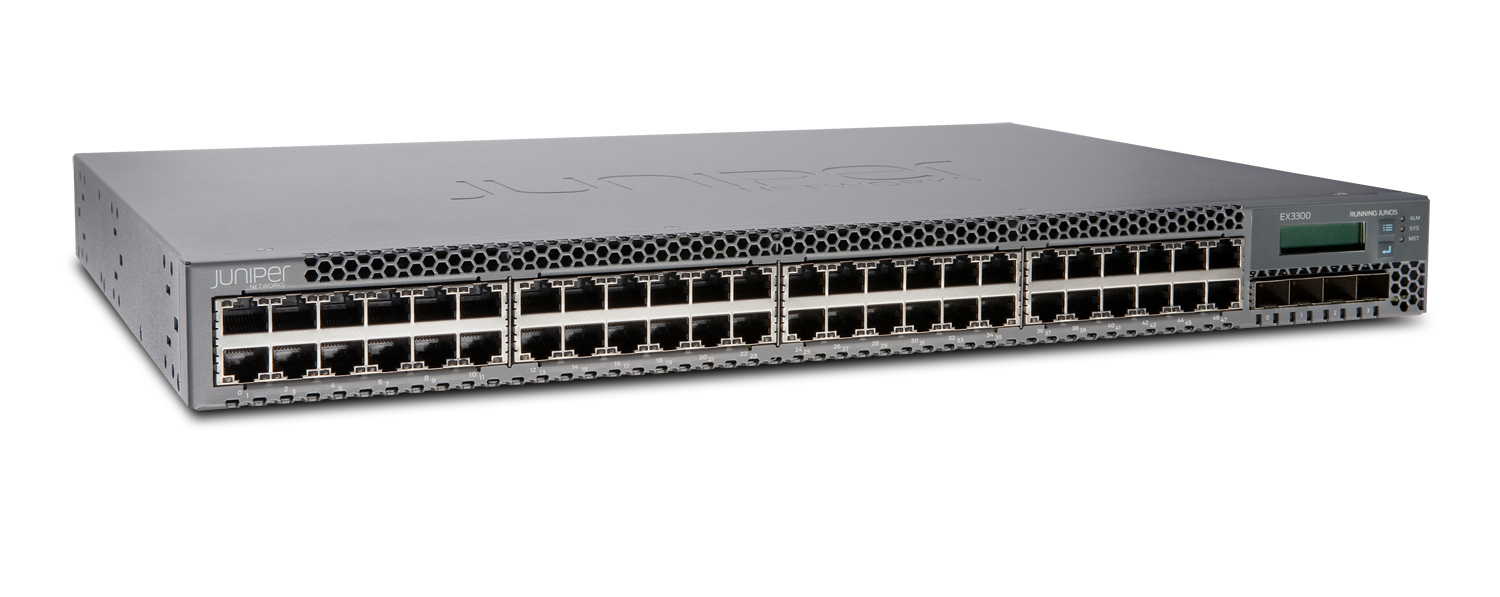
\includegraphics[width=\textwidth]{images/ethernetswitch.jpg}
    \caption{Een Ethernetswitch met 48 poorten en 4 openingen voor SFP-modules}
    \label{fig:ethernetswitch}
\end{figure}


In \vref{fig:simple-lan} zijn drie computers met elkaar verbonden via een switch.
Computer~1 wil communiceren met computer~2.
We gaan er even van uit dat beide computers elkaars IP-adres en MAC-adres kennen.
Als de switch de eerste frame ontvangt van computer~1, weet het nog niets over het netwerk of de toestellen die verbonden zijn met de switch, dus stuurt het het frame via alle interfaces naar buiten.
Computers~2 en~3 ontvangen dus dit eerste frame.
Computer~3 ziet het destination MAC-adres van het frame en, omdat dit niet zijn MAC-adres is, gooit het frame weg.
Computer~2 herkent wel zijn eigen MAC-adres in het frame en verwerkt de inhoud en stuurt uiteindelijk een antwoord terug.

De switch stuurt niet alleen het frame aan alle interfaces naar buiten, maar maakt ook notitie van het source MAC-adres en noteert dit in de MAC-tabel samen met de interface waarop hij het MAC-adres geleerd heeft.
\begin{center}
\begin{tabular}{cc}
\textit{MAC-adres} & \textit{interface} \\[1ex]
0200.aaaa.0001 & fa0/1\\
\end{tabular}
\end{center}
Als computer~2 nu een antwoord stuurt naar computer~1, komt dit frame aan op fa0/2 van de switch.
Weer noteert de switch het source MAC-adres in de MAC-tabel samen met de interface waarop de switch het frame ontvangt.
Vervolgens zoekt de switch het destination MAC-adres op in de MAC-tabel, vindt de bijhorende interface, en verstuurt het frame enkel langs deze interface naar buiten.
Computer~3 ziet dit antwoord -- en alle verder communicatie tussen computers~1 en~2 -- niet meer.

\begin{figure}
    \centering
    \documentclass[tikz]{standalone}
\usepackage{ifthen}
\usepackage{contour}
\input{../tex/mdt-colors}
\input{../pgf/tikz-pgf}
\input{../pgf/layers}
\input{../pgf/connections}
\input{../pgf/nodes}
\begin{document}
\begin{tikzpicture}[framed]
\def\iconset{basic}
%\showhostnamesinterfaces
\nodeswitch[bottom]{switch}{3,0}{Cisco 2960}{}
\nodehost[left]{pc 1}{0,0}{FreeBSD}{0200.aaaa.0001}
\nodehost{pc 2}{6,0}{FreeBSD}{0200.aaaa.0002}
\nodehost{pc 3}{3,3}{Linux}{0200.aaaa.0003}
\connect{switch}{fa0/1}{pc 1}{em0}
\connect{switch}{fa0/2}{pc 2}{em0}
\connect{switch}{fa0/3}{pc 3}{eth0}


\end{tikzpicture}
\end{document}
    \caption{Een eenvoudig netwerk met twee computers die met elkaar verbonden zijn via een switch}
    \label{fig:simple-lan}
\end{figure}

Een MAC-adres kan slechts aan één interface gekoppeld zijn.
Als de switch een MAC-adres dat het al kent, opnieuw leert via een andere interface, dan update het de bestaande entry in de MAC-tabel door de oude interface te vervangen door de nieuwe interface.

Het is wel mogelijk dat meerdere MAC-adressen op dezelfde interface geleerd worden.
Dit is mogelijk als een computer met meerdere virtuele machines, verbonden wordt met de switch.
Elke virtuele machine heeft immers een eigen MAC-adres.
Het is ook mogelijk meerdere MAC-adressen te leren op een interface als deze interface met een andere switch verbindt.
De eerste switch leert dan de MAC-adressen van alle computers die verbinden met de tweede switch via deze interface.


\section{Lussen in het netwerk}
\label{sec:stp}

Als één switch niet meer voldoende is om alle computers en printers met elkaar te verbinden, verbinden we een tweede switch met de eerste switch.
Als beide switch niet meer voldoende zijn, kunnen we nog een derde switch verbinden met het netwerk, en vervolgens nog een vierde en vijfde switch (zie \vref{fig:daisy-chain}).
Een dergelijk netwerk kan lang goed functioneren.
Tot op een dag bijvoorbeeld switch~2 kapot gaat en alle computers die met switches~3 tot en met~5 verbonden zijn, geen Internetconnectiviteit meer hebben.
Maar dit is eenvoudig op te lossen.
We verbinden switch~1 snel met switch~3 en de connectiviteit is hersteld.


\begin{figure}
    \centering
    \documentclass[tikz]{standalone}
\usepackage{ifthen}
\usepackage{contour}
\input{../tex/mdt-colors}
\input{../pgf/tikz-pgf}
\input{../pgf/layers}
\input{../pgf/connections}
\input{../pgf/nodes}
\begin{document}
\begin{tikzpicture}[framed]
\def\iconset{basic}
\nodecloud{Internet}{0,4}{}{}
\nodefirewall{firewall}{0,2}{}{}
\nodeswitch[bottom]{sw1}{0,0}{}{}
\nodeswitch[bottom]{sw2}{2,0}{}{}
\nodeswitch[bottom]{sw3}{4,0}{}{}
\nodeswitch[bottom]{sw4}{6,0}{}{}
\nodeswitch[bottom]{sw5}{8,0}{}{}
\connect{Internet}{}{firewall}{}
\connect{firewall}{}{sw1}{}
\connect{sw1}{}{sw2}{}
\connect{sw2}{}{sw3}{}
\connect{sw3}{}{sw4}{}
\connect{sw4}{}{sw5}{}
\end{tikzpicture}
\end{document}
    \caption{Meerdere switches worden met elkaar verbonden in een lange lijn. Dit noemt \emph{daisy chaining}.}
    \label{fig:daisy-chain}
\end{figure}


Dit brengt echter een groot gevaar met zich mee.
Zolang switch~2 defect blijft, is er niets aan de hand.
Maar zodra switch~2 vervangen wordt door een nieuwe switch, hebben we een lus gemaakt in het netwerk.
Switch~1 verbindt met switch~2, zo met switch~3 en dan opnieuw naar switch~1.
Dit lijkt onschadelijk maar is dat zeker niet.

Neem opnieuw een computer verbonden met switch~1.
Deze wil met een andere computer in het netwerk communiceren.
De MAC-tabellen van alle drie de switches zijn leeg.
Als het eerste frame van de computer aankomt op switch~1, kan deze het source MAC-adres invullen zijn MAC-tabel maar omdat hij het destination MAC-adres niet kent, stuurt hij het frame via alle interfaces naar buiten.
Dit frame komt dus zowel bij switch~2 als bij switch~3 aan.
Switch~2 heeft ook een lege MAC-tabel dus stuurt het frame ook aan alle interfaces naar buiten, dus ook naar switch~3.

Switch~3 ontvangt het frame dus twee keer, een keer van switch~1 en een keer van switch~2.
Omdat het destination MAC-adres nog altijd niet bekend is, stuurt de switch beide frames langs alle interfaces naar buiten.
Switch~3 stuurt het frame dat hij van switch~2 gekregen heeft, door naar switch~1 en stuurt het frame van switch~1 door naar switch~2.

Eén frame heeft zich via deze lus verdubbeld en deze twee frames blijven rondlussen in het netwerk.
Dit soort fysieke lussen in het netwerk, kunnen een netwerk snel op de knieën brengen.



\section{Spanning-tree protocol (STP)}
Deze fysieke lussen zijn goed.
Als een switch of kabel kapot gaat, hebben de computers nog steeds netwerkconnectiviteit via de andere route.
Maar door de manier waarop switches omgaan met BUM-verkeer (broadcast, unknown unicast, multicast -- voor deze drie types heeft een switch nooit het destination MAC-adres in de MAC-tabel) zijn deze fysieke lussen net schadelijk voor je netwerk.
Het \emph{spanning-tree protocol} (STP) is een protocol dat deze fysieke lussen detecteert en telkens één interface in de lus uitschakelt.
Op die manier is het gevaar geweken want de frames kunnen niet meer eindelijk rondjes blijven draaien in de lus.
Als er echter een switch of kabel kapot gaat, wordt dit gedetecteerd door STP en wordt de interface die werd uitgezet, terug aangezet.

Spanning-tree protocol doet dit met behulp van \emph{bridge protocol data units} (BPDU),%
    \footnote{%
        De term ``bridge'' is een oude term voor ``switch.''
        Er waren enkele technische verschillen tussen beide soorten toestellen maar nu kunnen beide termen door elkaar gebruikt worden.%
        In de technische documentatie rondom STP wordt nog steeds bijna uitsluitend de term ``bridge'' gebruikt.
    }
speciale frames die switches naar elkaar sturen om informatie uit te wisselen over de status van het netwerk.
STP doorloopt vier stappen om een \emph{loop-free network} te bekomen.
\begin{enumerate}
\item
    Beslis samen welke switch de \emph{root bridge} wordt van het netwerk.
    Deze switch is als het ware de baas en verstuurt de BPDU's waarop de andere switches hun keuzes baseren.
    We kunnen de root bridge ook zien als de stam van de boom waar alle andere switches en verbindingen van aftakken.
\item
    Elke switch bepaalt de kortste route naar de root bridge en markeert deze interface als de \emph{root port}.
\item
    Elke link (kabel die twee switches met elkaar verbindt) heeft één \emph{designated port}.
    Als een van beide uiteindes al een root port is, moet de andere kant de designated port zijn.
    Als geen van beide uiteindes de root port is, wordt op basis van een selectiecriterium bepaald welk van de twee de designated port wordt.
\item
    Elke interface die geen root port of designated port is, wordt uit gezet.
    Op deze manier worden alle lussen in het netwerk verbroken.
\end{enumerate}

In stappen~1 en~3 moeten de switches een keuze maken.
Deze wordt gemaakt op basis van de volgende criteria.

LALALA NOT COMPLETE TODO


\section{Virtuele switches}


\section{Virtuele kabels}

% Ik heb geen idee wat ik bedoelde met virtuele kabels...
\Chapter{Wires and wireless}
\label{chap:wires-wireless}

\Section{Wires}
\label{sec:wires}

\Paragraph{twisted pair}
\mode<article>{
Twisted pair cabling is a type of wiring in which two conductors of a single circuit are twisted together for the purposes of improving electromagnetic compatibility.
Compared to a single conductor or an untwisted balanced pair, a twisted pair reduces electromagnetic radiation from the pair and crosstalk between neighbouring pairs and improves rejection of external \ac{EMI}.
It was invented by Alexander Graham Bell.
}

\Paragraph{shielded vs unshielded}
\mode<article>{
For additional noise immunity, twisted-pair cabling may be shielded.
Cable with shielding is known as \ac{ShTP} and without as \ac{UTP}.

Common shield construction types include \emph{individual} shielding (\abbr{U/\-FTP}) with aluminium foil for each twisted pair or quad.
This type of shielding helps prevent \ac{EMI} from entering or exiting individual pairs and also protects neighbouring pairs from crosstalk.
\emph{Overall} shielding with overall foil (\abbr{F/UTP}), braided shield (\abbr{S/UTP}), or braiding with foil across all of the pairs (\abbr{SF/UTP}).
This type of shielding helps prevent \ac{EMI} from entering or exiting the cable.

Finally, there is \emph{individual and overall} shielding which uses individual shielding using foil between the twisted pair sets, and also an outer foil or braided shielding (\abbr{F/FTP}, \abbr{S/FTP}, and \abbr{SF/FTP}).
This type of shielding helps prevent \ac{EMI} from entering or exiting the cable and also protects neighbouring pairs from crosstalk.
}

\Paragraph{categories}
\mode<article>{
There are different categories of twisted pair cabling.
Each category must adhere to a different standard and stringent specifications for crosstalk and system noise.
These standard specify the maximum distance a cable must be able to cover, the bandwidth, and the required shielding.

See \vref{tab:tp-categories} for an overview of the different categories.


\begin{table}
   \caption{Twisted pair categories}
   \label{tab:tp-categories}
   \centering
   \sffamily
   \begin{tabular}{lrrl}
   \textbf{cat.} & \textbf{dist. (m)} & \textbf{\textsc{BW} (MHz)} & \textbf{application} \\[1ex]
   3 & 100 & 16 & \abbr{10BASE-T} \\
   4 &     & 20 & Token Ring \\
   5 & 100 & 100 & \abbr{1000BASE-T} \\
   5e & 100 & 100 & \abbr{1000BASE-T}, \abbr{2.5GBASE-T} \\
   6  & 55  & 250 & \abbr{10GBASE-T} \\
   $6_\mathrm{A}$ & 100 & 500 & \abbr{10GBASE-T} \\
   7 & 100 & 600 & \abbr{10GBASE-T} \\
   $7_\mathrm{A}$ & & 1000 & \\
   8.1 & 36 & 2000 & \abbr{40GBASE-T} \\
   8.2 & 36 & 2000 & \abbr{40GBASE-T} \\
   \end{tabular}
\end{table}
}

\Paragraph{\acs{RJ45}}
\mode<article>{
The connector used for network cables is actually called an \acs{8P8C} connector but everyone knows it as a \acs{RJ45} connector.
A completely plastic connector is used for unshielded cabling while a metalic version exists for shield cabling.

\begin{figure}
   \centering
   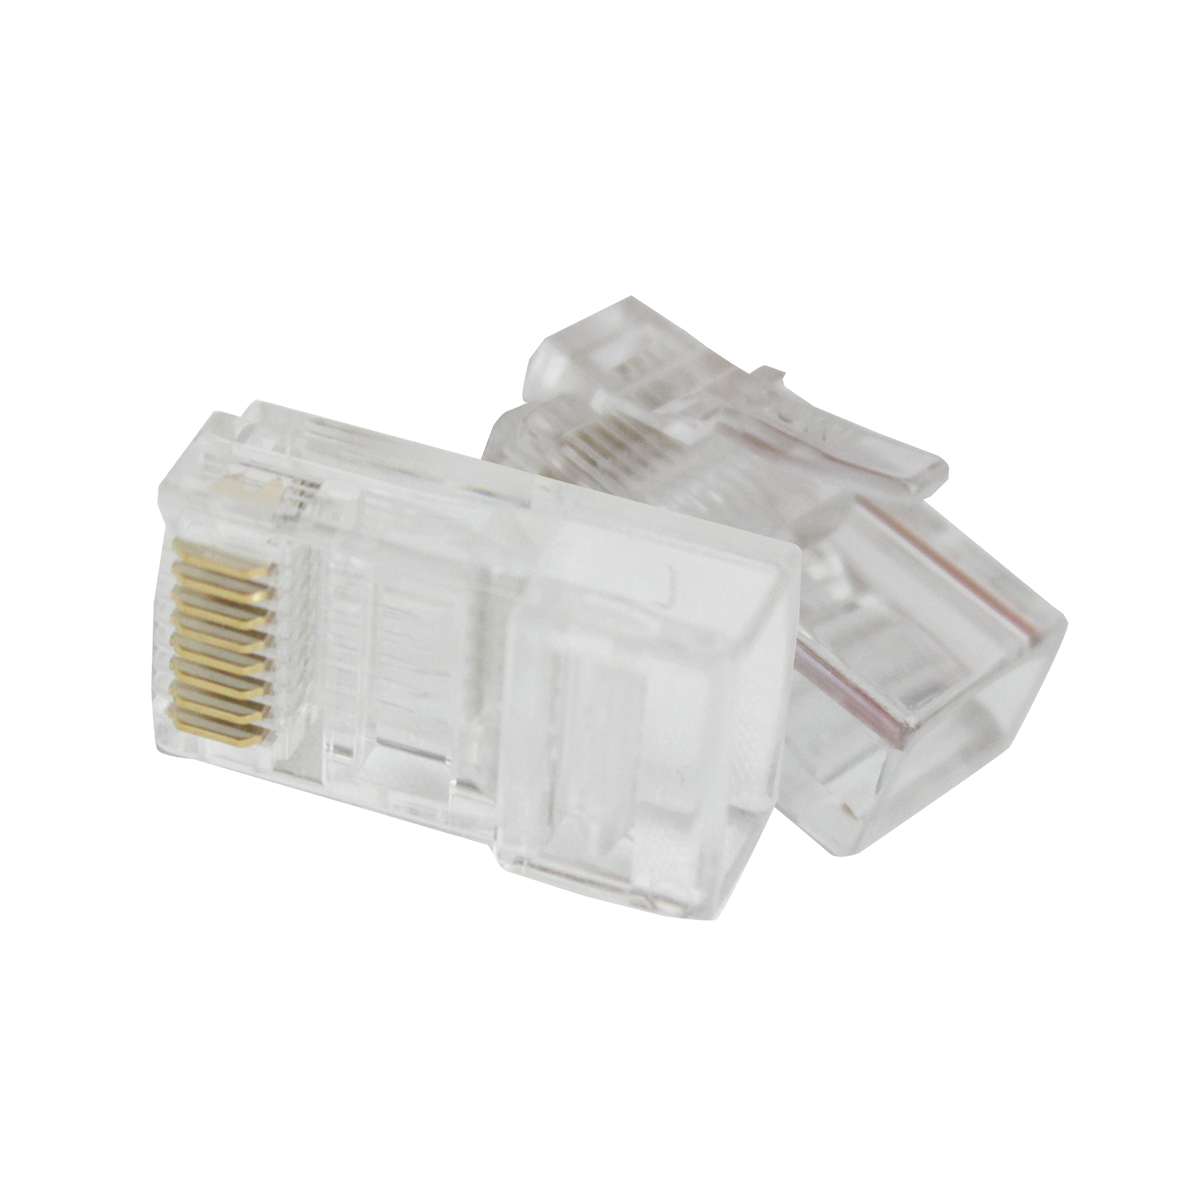
\includegraphics[width=.5\textwidth]{images/8p8c.png}
   \caption{Two plastic \acs{RJ45} connectors used with unshielded cabling}
   \label{fig:rj45}
\end{figure}
}
\slide{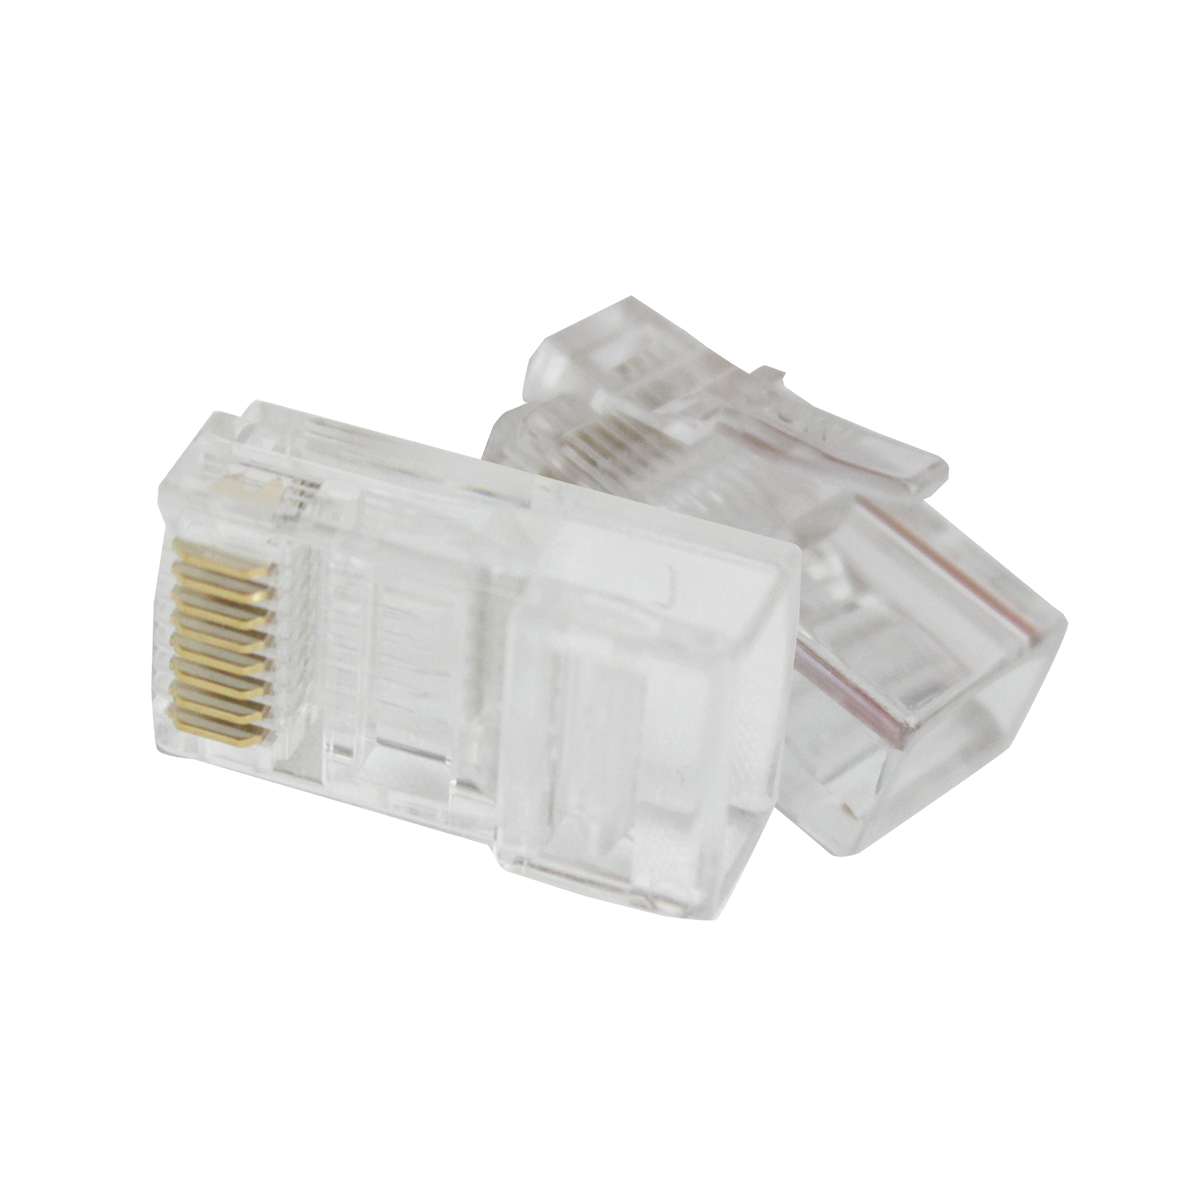
\includegraphics[width=.7\textwidth]{images/8p8c.png}}

\Paragraph{Fast Ethernet}
\mode<article>{
\abbr{100BASE-TX} is the predominant form of Fast Ethernet, and runs over two wire-pairs inside a category~5 or above cable.
Each network segment can have a maximum cabling distance of \SI{100}{\metre}.
One pair is used for each direction, providing full-duplex operation with \SI{100}{\mega\bit\per\second} of throughput in each direction.
Like \abbr{10BASE-T}, the active pairs in a standard connection are terminated on pins 1,~2,~3 and~6.
Since a typical category~5 cable contains 4~pairs, it can support two \abbr{100BASE-TX} links with a wiring adaptor.
}

\Paragraph{crossover cable}
\mode<article>{
An Ethernet crossover cable is a crossover cable for Ethernet used to connect computing devices together directly.
It is most often used to connect two devices of the same type, e.g. two computers (via their network interface controllers) or two switches to each other.
By contrast, \emph{straight-through} patch cables are used to connect devices of different types, such as a computer to a network switch.
Intentionally crossed wiring in the crossover cable connects the transmit signals at one end to the receive signals at the other end.
Many network devices today support auto-\acs{MDI-X} (aka auto-crossover) capability, wherein a patch cable can be used in place of a crossover cable, or vice versa, and the receive and transmit signals are reconfigured automatically within the device to yield a working connection.

To make a straight-through patch cable, either use the order defined by \abbr{T568A} on both ends of the cable, or the order defined by \abbr{T568B}.
To create a crossover patch cable, use \abbr{T568A} on one side and \abbr{T568B} on the other.

\begin{figure}
\centering
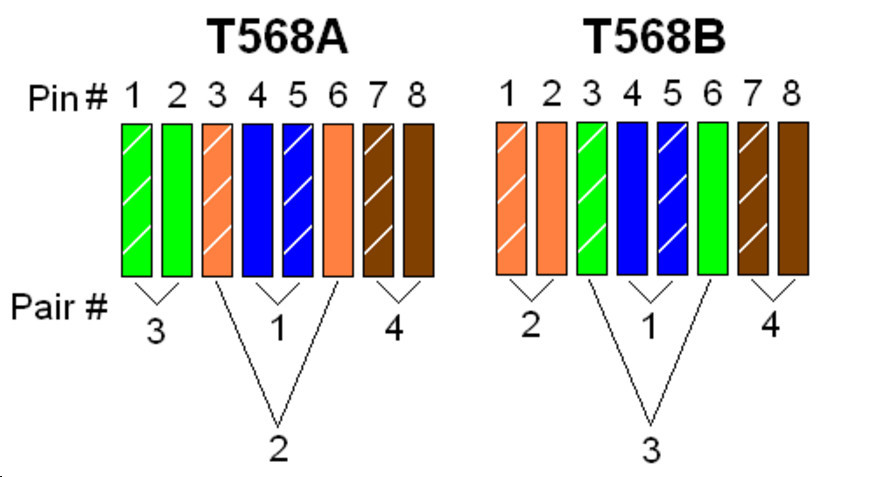
\includegraphics[width=.7\textwidth]{images/t568.jpeg}
\caption{The \abbr{T568} standard for twisted-pair cabling}
\label{fig:t568}
\end{figure}

% TODO: explain (with a drawing?) that pair 1/3 is used for sending and the other for receiving data.
}

\Paragraph{Gigabit Ethernet}
\mode<article>{
In computer networking, Gigabit Ethernet (GbE or 1~GigE) is the term applied to transmitting Ethernet frames at a rate of a gigabit per second.
The most popular variant \abbr{1000BASE-T} is defined by the \acs{IEEE} 802.3ab standard.
It came into use in 1999, and has replaced Fast Ethernet in wired local networks due to its considerable speed improvement over Fast Ethernet, as well as its use of cables and equipment that are widely available, economical, and similar to previous standards.

Each \abbr{1000BASE-T} network segment is recommended to be a maximum length of 100~metres, and must use Category~5 cable or better (including Cat~5e and Cat~6).
In a departure from both \abbr{10BASE-T} and \abbr{100BASE-TX}, \abbr{1000BASE-T} uses four lanes over all four cable pairs for simultaneous transmission in both directions.
}

\Paragraph{auto \acs{MDI-X}}
\mode<article>{
Auto \acs{MDI-X} (aka `auto crossover') automatically detects the required cable connection type and configures the connection appropriately, removing the need for crossover cables to interconnect switches or connecting \acsp{PC} peer-to-peer.
As long as it is enabled on either end of a link, either type of cable can be used.
For auto \acs{MDI-X} to operate correctly, the data rate on the interface and duplex setting must be set to `auto.'

Gigabit and faster Ethernet links over twisted pair cable use all four cable pairs for simultaneous transmission in both directions.
For this reason, there are no dedicated transmit and receive pairs, and consequently, crossover cables are never required for \abbr{1000BASE-T} communication.
}

\Paragraph{100\,Gbit Ethernet}
\mode<article>{
Using Cat.~8 twisted pair cabling it is possible to go up to \SI{40}{\giga\bit\per\second} using cables up to \SI{30}{\metre}.
Higher speeds or longer lengths require fibre optic cables to be used.
}

\Paragraph{\acl{DAC}}
\mode<article>{
A \acf{DAC} cable is a copper 10~Gigabit Ethernet cable which comes in either an active or passive twinax (twinaxial) cable assembly and connects directly into an \acs{SFP+} housing (\vref{fig:dac}).
\abbr{40GBASE-CR4} and \abbr{100GBASE-CR10} physical layers using \SI{7}{\metre} twin-axial cable are being developed as part of the 100~Gbit Ethernet specifications by the \acs{IEEE}.

\begin{figure}
\centering
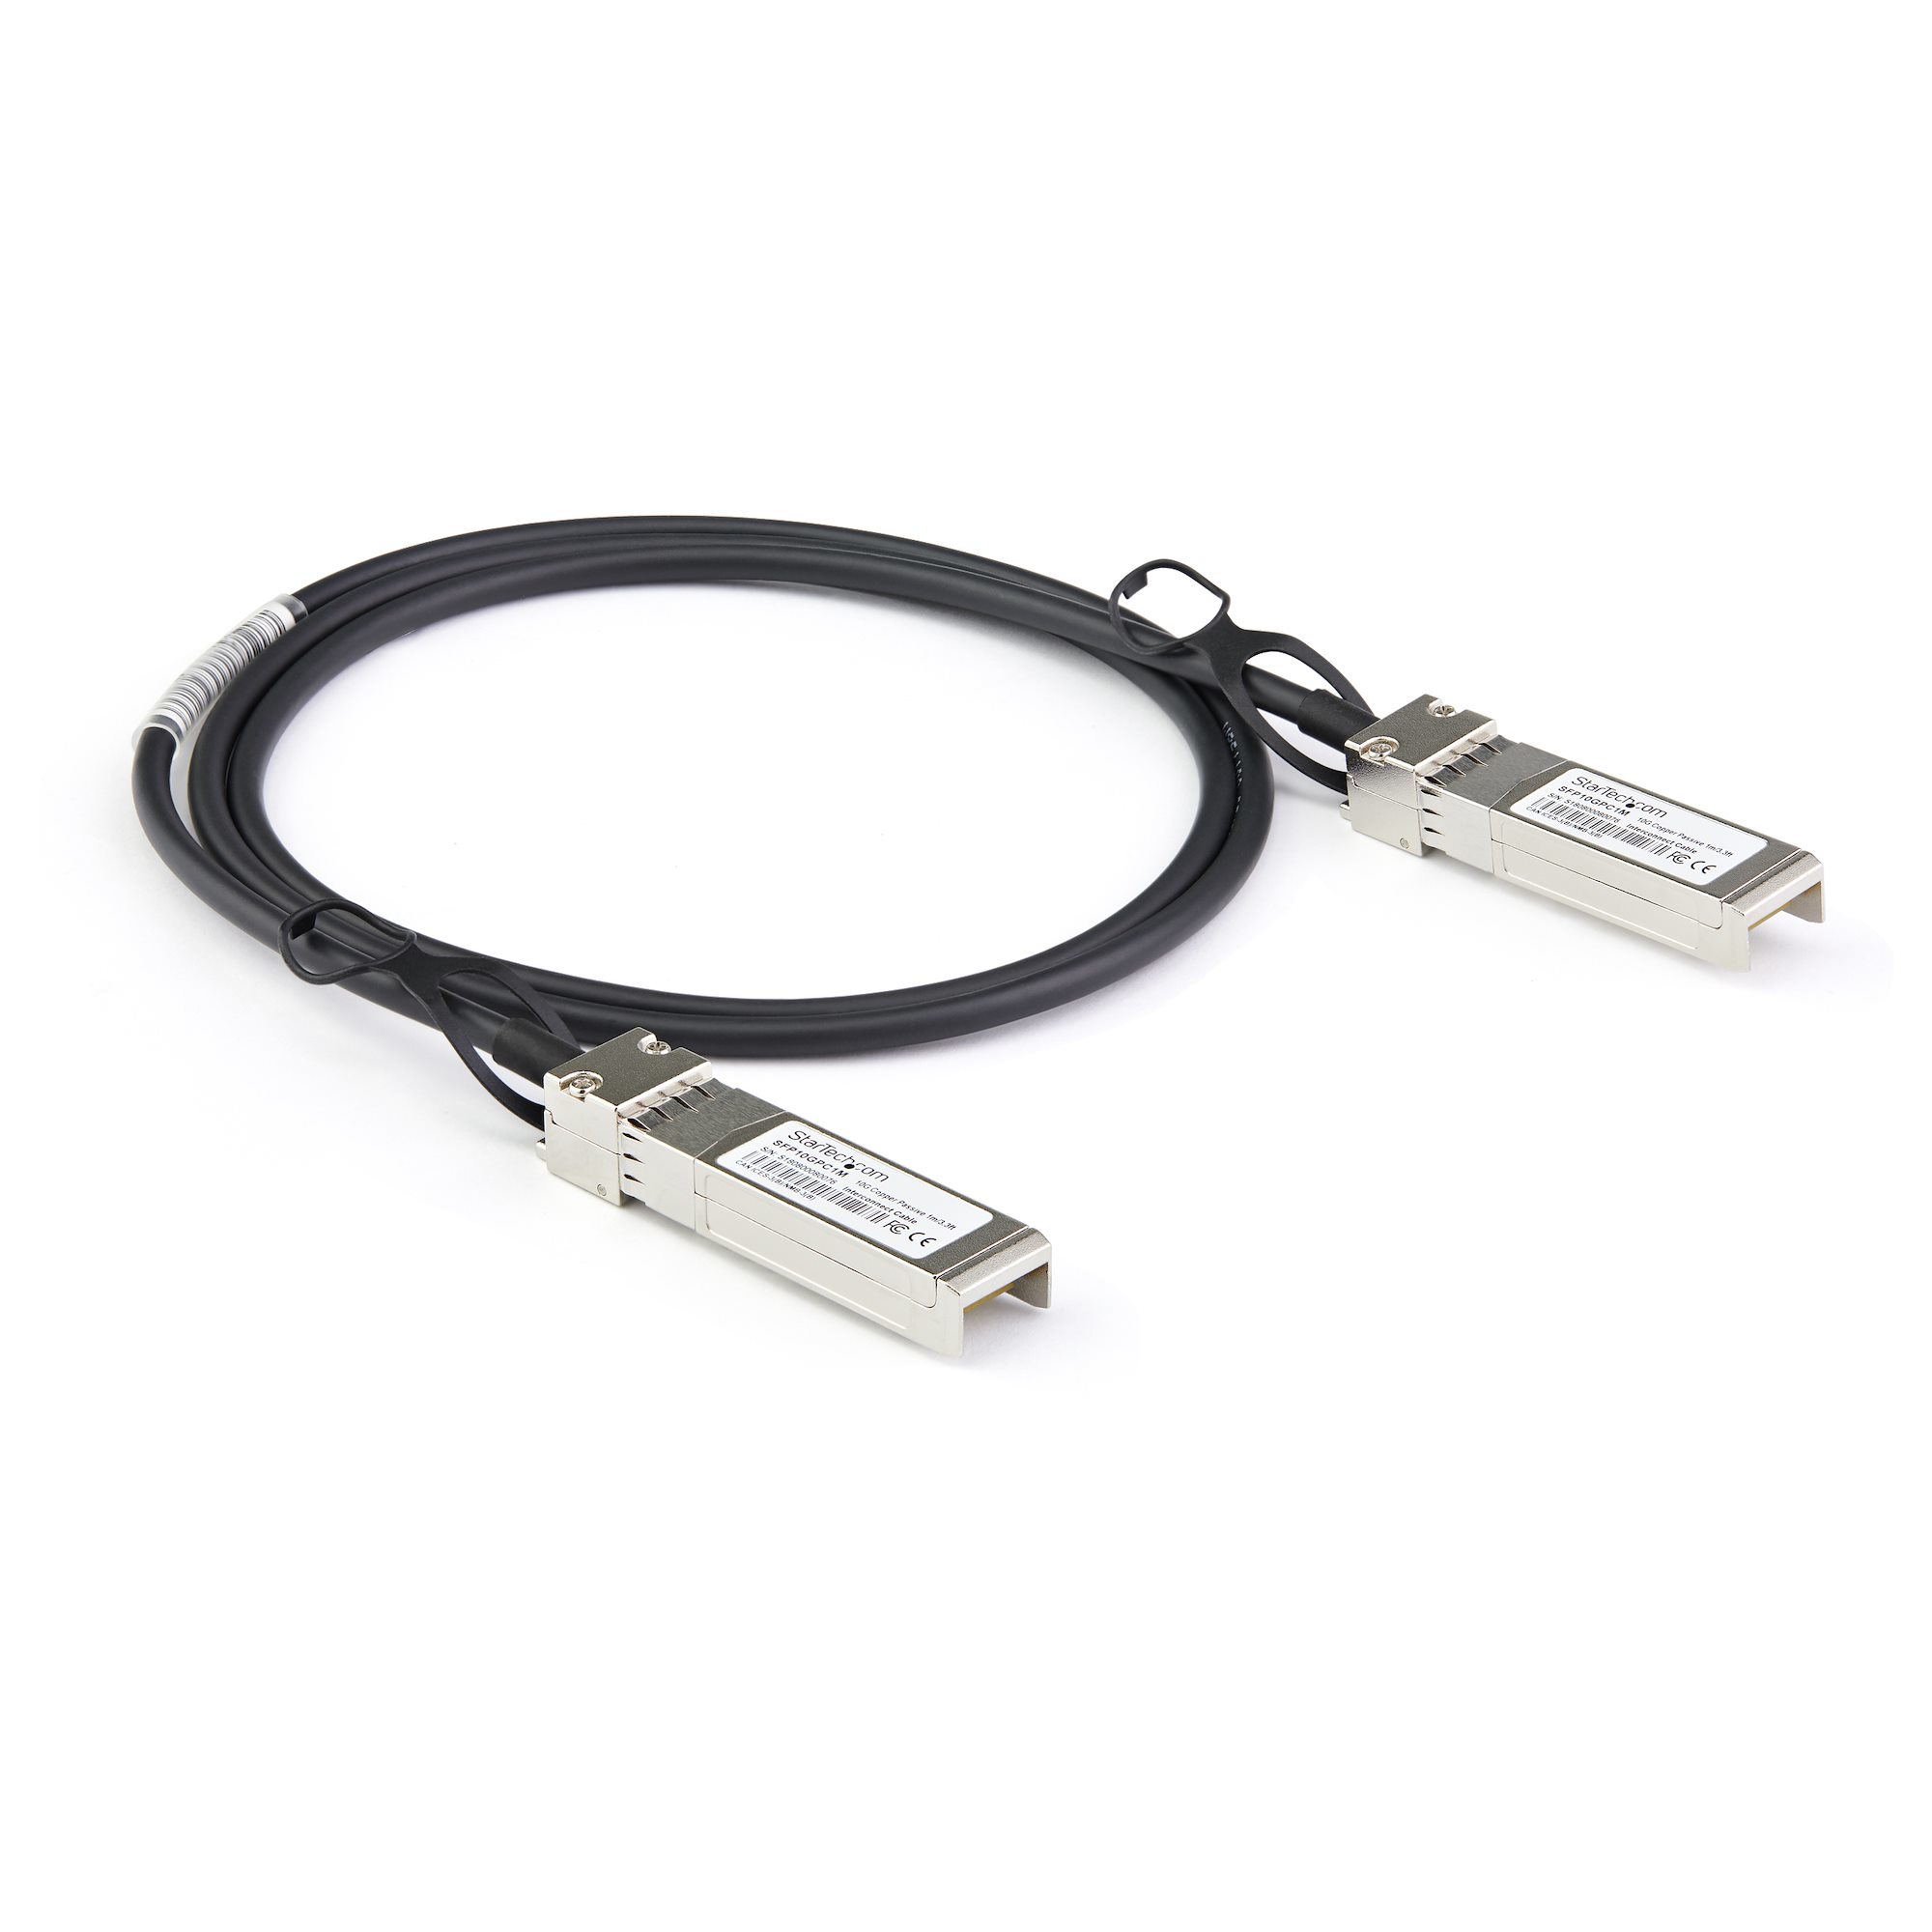
\includegraphics[width=.7\textwidth]{images/dac-cable.jpeg}
\caption{A direct-attach copper cable}
\label{fig:dac}
\end{figure}
}

\Paragraph{optical fibre}
\mode<article>{
An optical fibre is a flexible, transparent fibre made by drawing glass (silica) or plastic to a diameter slightly thicker than that of a human hair.
Fibres are used instead of metal wires because signals travel along them with less loss; in addition, fibres are immune to electromagnetic interference, a problem from which metal wires suffer.
The concept of a direct-attech copper cable also exist with optical cables.
These are then called \acf{AOC}.

\begin{table}
   \caption{Fibre optic categories}
   \label{tab:fo-categories}
   \centering
   \sffamily
   \begin{tabular}{lrrll}
   \textbf{cat.} & \textbf{core ($\bm{\mathrm{\upmu{}m}}$)} & {\small\textbf{\abbr{BW} (MHz)}} & \textbf{color} & \textbf{Ethernet standard} \\[1ex]
   \abbr{OM1} & 62.5    &  200 & orange & {\small \abbr{10GBASE-SR} (\SI{33}{\metre})} \\
   \abbr{OM2} & 50      &  500 & orange & {\small \abbr{10GBASE-SR} (\SI{82}{\metre})} \\
   \abbr{OM3} & 50      & 2000 & aqua   & {\small \abbr{100GBASE-SR4} (\SI{100}{\metre})} \\
   \abbr{OM4} & 50      & 4700 & aqua   & {\small \abbr{100GBASE-SR4} (\SI{150}{\metre})}\\
   \abbr{OS1} & 8--10.5 &      & yellow & {\small \abbr{100GBASE-ER4} (\SI{40}{\kilo\metre})} \\
   \abbr{OS2} & 8--10.5 &      & yellow & {\small \abbr{100GBASE-ER4} (\SI{40}{\kilo\metre})} \\
   \end{tabular}
\end{table}
}

\Paragraph{single-mode}
\mode<article>{
In fibre-optic communication, a \ac{SMF}, also known as fundamental- or mono-mode, is an optical fibre designed to carry only a single mode of light -- the transverse mode.
Waves can have the same mode but have different frequencies. This is the case in single-mode fibres, where we can have waves with different frequencies, but of the same mode, which means that they are distributed in space in the same way, and that gives us a single ray of light.
}

\Paragraph{multi-mode}
\mode<article>{
Multi-mode optical fibre is a type of optical fibre mostly used for communication over short distances, such as within a building or on a campus.
Multi-mode links can be used for data rates up to \SI{100}{\giga\bit\per\second}.
Multi-mode fibre has a fairly large core diameter that enables multiple light modes to be propagated and limits the maximum length of a transmission link because of modal dispersion.
}

\Paragraph{transceivers}
\mode<article>{
As there are so many different options regarding transceivers depending on bandwidth, distance and the use of lasers or \acsp{LED}, network equipment does not have built-in transceivers.
It is more convenient to have a modular system where you can plug in the transceiver you need.
There are different form factors available, including \acs{SFP}, \acs{SFP+} and \acs{QSFP}.

\begin{figure}
   \begin{subfigure}[b]{0.45\textwidth}
   \centering
   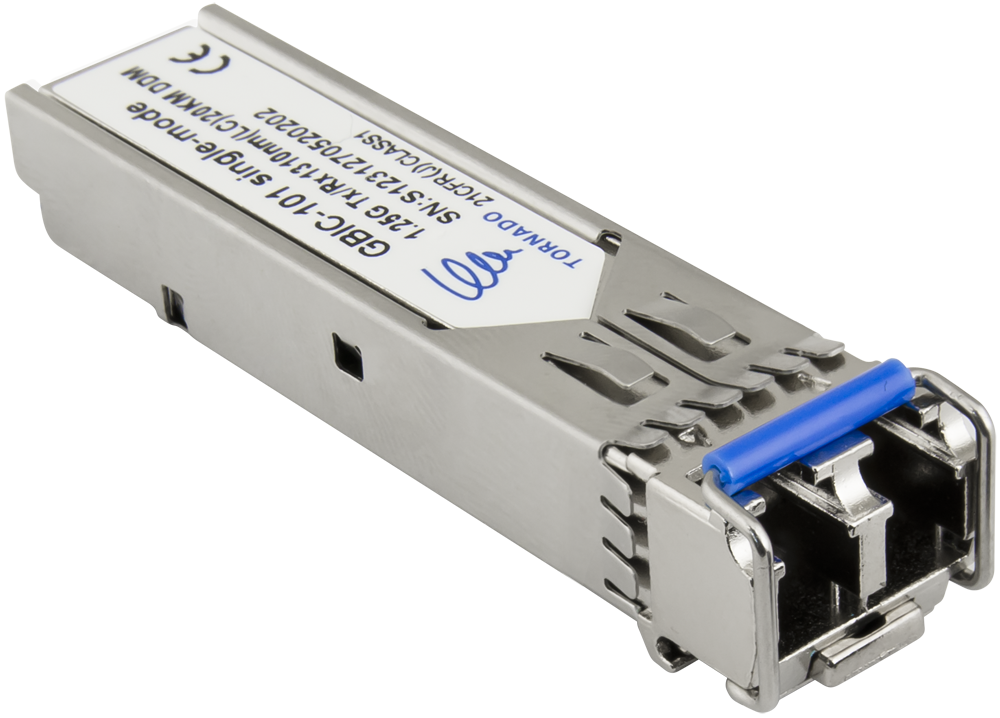
\includegraphics[width=\textwidth]{images/sfp.png}
   \caption{An \acs{SFP} with an \acs{LC} connector}
   \label{fig:sfp-lc}
   \end{subfigure}
   \hfill
   \begin{subfigure}[b]{0.45\textwidth}
   \centering
   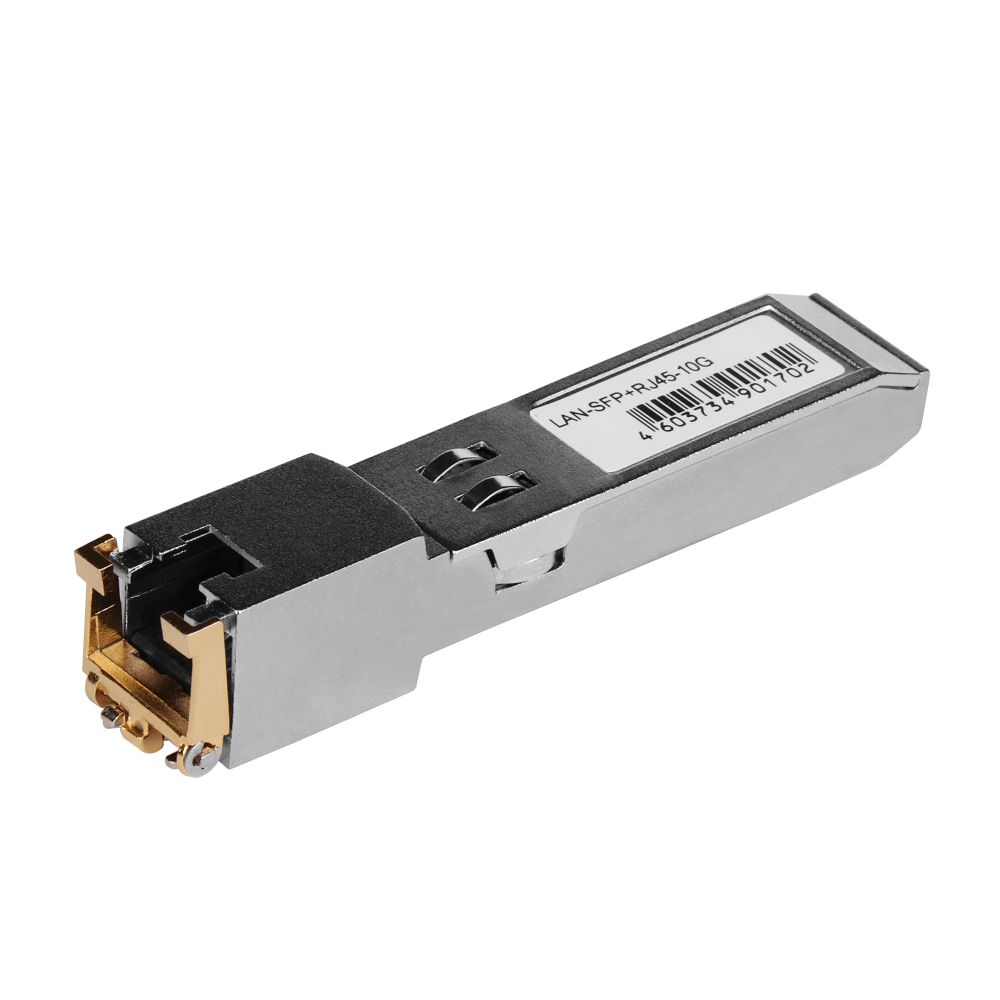
\includegraphics[width=\textwidth]{images/sfp-rj45.png}
   \caption{An \acs{SFP} with a \acs{RJ45} connector}
   \label{fig:sfp-rj45}
   \end{subfigure}
   \caption{Two small \acf{SFP} transceivers}
   \label{fig:sfp}
\end{figure}

Nowadays most connectors are \acs{LC} (as in \vref{fig:sfp}) but in data centres \acs{MPO} cables (\vref{fig:mpo}) are also used for high-speed connections and for interconnecting patch panels.
An \acs{MPO} cable can have up to 72 fibre strands in a cable.
See also \href{https://www.qsfptek.com/article/fiber-connector-types-lc-sc-fc-st-mtp-mpo}{qsfptek.com} for more information on different fibre optic connectors.

\begin{figure}
   \centering
   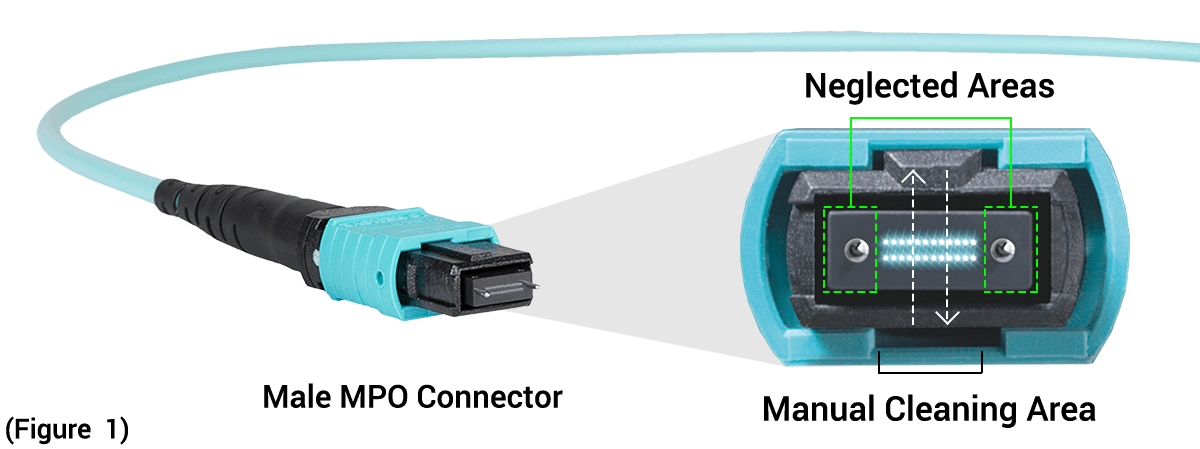
\includegraphics[width=\textwidth]{images/mpo.png}
   \caption{\acs{MPO} connnector}
   \label{fig:mpo}
\end{figure}

\begin{figure}
   \centering
   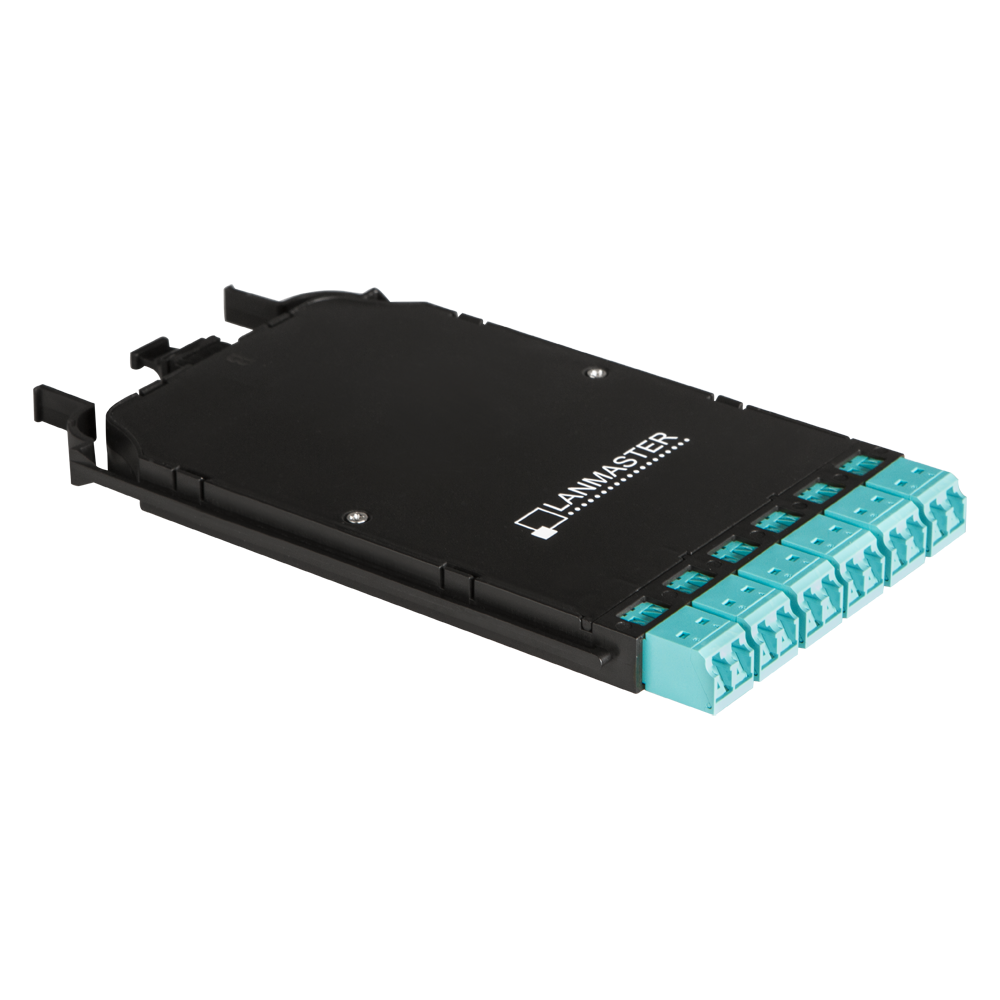
\includegraphics[width=.5\textwidth]{images/mpo-cassette.png}
   \caption{\acs{MPO} cassette}
   \label{fig:mpo-cassette}
\end{figure}
}
\slide{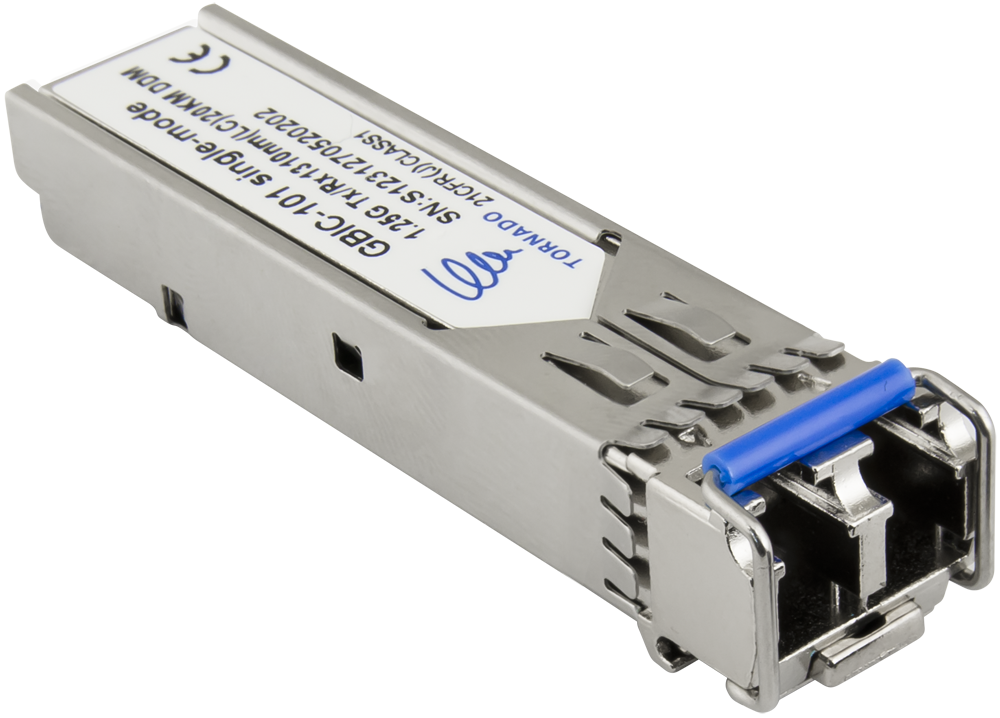
\includegraphics[width=.7\textwidth]{images/sfp.png}}
\slide{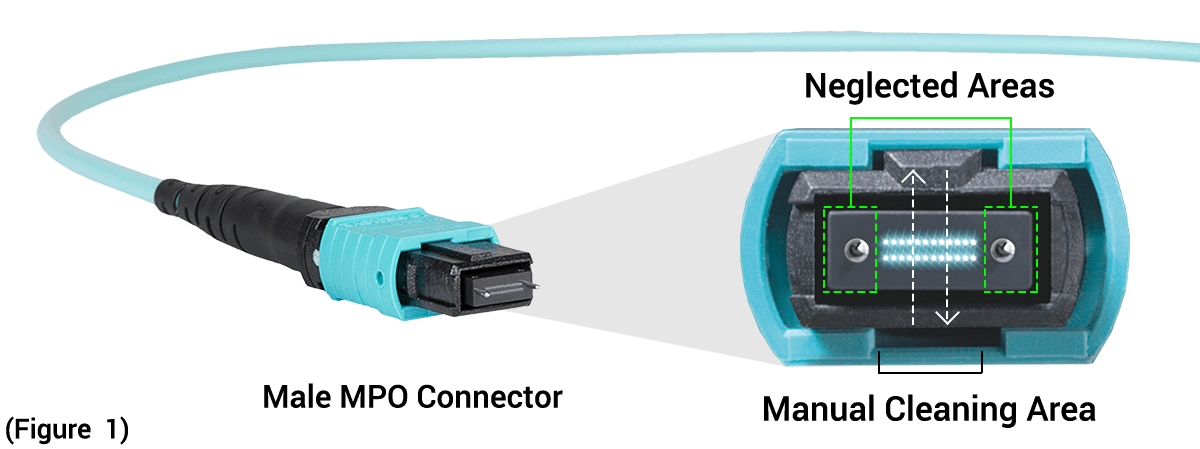
\includegraphics[width=.7\textwidth]{images/mpo.png}}
\slide{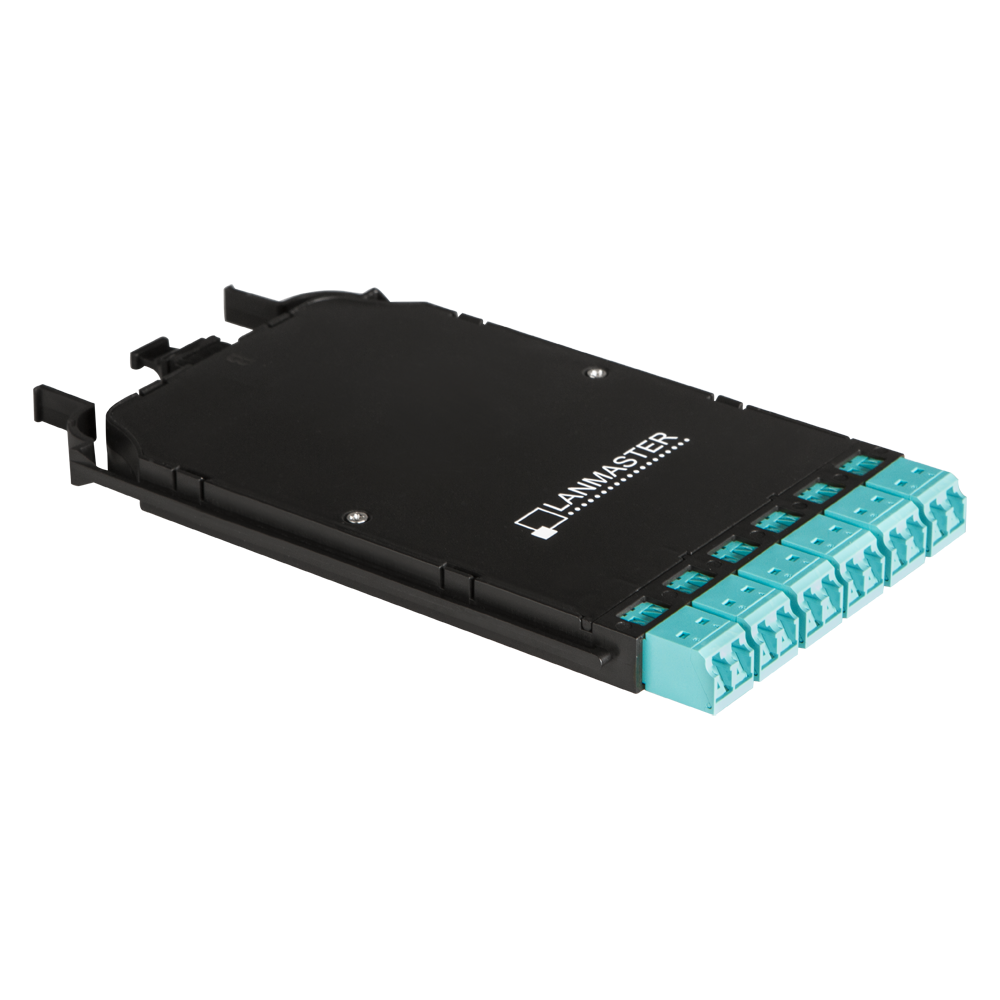
\includegraphics[width=.7\textwidth]{images/mpo-cassette.png}}






\Section{Wireless}
\label{sec:wireless}

\Paragraph{802.11}
\mode<article>{
\acs{IEEE} 802.11 specifies the set of \acf{MAC} and physical layer (\abbr{PHY}) protocols for implementing \acf{WLAN} computer communication.
The standard and amendments provide the basis for wireless network products using the Wi-Fi brand and are the world's most widely used wireless computer networking standards.

\begin{table}
   \centering
   \sffamily
   \begin{tabular}{lrrrl}
   \textbf{standard} & \textbf{generation} & \textbf{max linkrate}   & \textbf{adoption} & \textbf{frequency} \\
                     &                     & {\small \textbf{(Mbps)}} &                   & {\small \textbf{(GHz)}} \\[1ex]
   802.11   & 0  &       2 & 1997 & 2.4 \\
   802.11a  & 2  &      54 & 1999 & 5   \\
   802.11b  & 1  &      11 & 1999 & 2.4 \\
   802.11g  & 3  &      54 & 2003 & 2.4 \\
   802.11n  & 4  &     600 & 2008 & 2.4/5 \\
   802.11ac & 5  &  6\,933 & 2014 & 5 \\
   802.11ax & 6  &  9\,608 & 2019 & 2.4/5 \\
            & 6\abbr{E} &  9\,608 & 2020 & 2.4/5/6 \\
   802.11be & 7  & 40\,000 & \emph{t.b.d.} & 2.4/5/6 \\
   \end{tabular}
   \caption{Wi-Fi generations}
   \label{fig:wifi-generations}
\end{table}
}

\Paragraph{frequency}
\mode<article>{
\acs{IEEE} 802.11 uses various frequencies including \SI{2.4}{\giga\hertz}, \SI{5}{\giga\hertz}, \SI{6}{\giga\hertz}, and \SI{60}{\giga\hertz} frequency bands.
Although \acs{IEEE} 802.11 specifications list channels that might be used, the radio frequency spectrum availability allowed varies significantly by regulatory domain.
}

\Paragraph{channel}
\mode<article>{
The \SI{2.4}{\giga\hertz} frequency supports eleven channels in the United States and thirteen channels in Europe and most of the world.
The \SI{5}{\giga\hertz} frequency supports over fifty channels, depending on the bandwidth used.

\begin{figure}
\centering
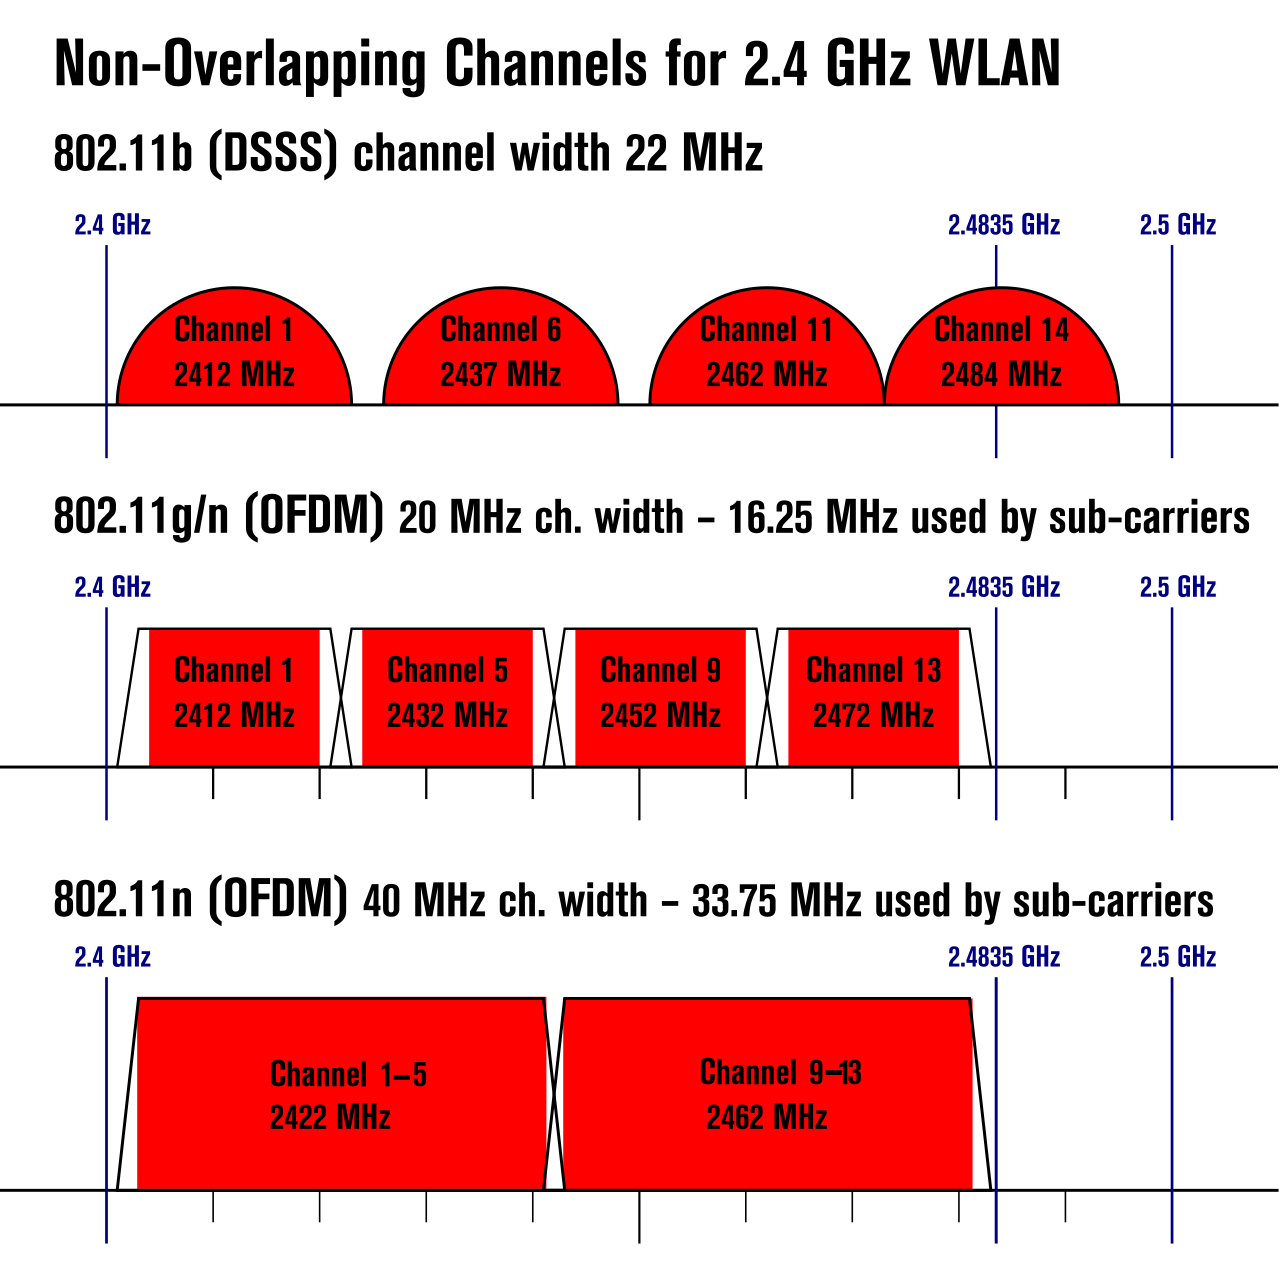
\includegraphics[width=.7\textwidth]{images/wifi-channels.png}
\caption{Non-overlapping wireless channels in the \SI{2.4}{\giga\hertz}-range}
\label{fig:wifi-channels}
\end{figure}
}

\Paragraph{bandwidth}
\mode<article>{
The bandwidth is one of the determinants of the capacity of a given communication channel.
Using a wireless channel with a bandwidth of \SI{40}{\mega\hertz} results in bigger speeds than a bandwidth of \SI{20}{\mega\hertz}.
However, when choosing the bandwidth, you have to make sure all devices that must connect to the wireless network do support this higher bandwidth.
}

\Paragraph{SSID}
\mode<article>{
The \ac{SSID} defines a service set or extended service set.%
\footnote{An \ac{ESS} is a wireless network, created by multiple access points, which appears to users as a single, seamless network, such as a network covering a home or office that is too large for reliable coverage by a single access point.}
Normally it is broadcast in the clear by stations in beacon packets to announce the presence of a network and seen by users as a wireless network name.
}

\Paragraph{antennas}
\mode<article>{
Professional access points are designed to be mounted upside down on the ceiling.
They radiate down into the room for a few metres and try to cover as much space on the floor as possible.
They are not designed to radiate upwards to the above floor or far down, to reach the floor below.

If you want to use such an access point to cover a large area in a garden, you would have to connect a different, external, antenna with a different coverage area.
}

\Paragraph{security}
\mode<article>{
Wi-Fi security includes \ac{WEP} and \ac{WPA}.
\ac{WEP} is a notoriously weak security standard: the password it uses can often be cracked in a few minutes with a basic laptop computer and widely available software tools.

There are two options available when chosing \ac{WPA}: personal mode and enterprise mode.
\ac{WPA} personal is also referred to as \acs{PSK} or \acl{PSK}.
This mode is designed for home and small office networks and does not require an authentication server.
Instead all users can access the wireless network using a common \acl{PSK}.

\ac{WPA} enterprise or \abbr{802.1X} requires a \ac{RADIUS} server for authentication.
This mode requires a more complicated setup, but provides additional security (e.g.\ protection against dictionary attacks on short passwords).
Most noticably, it requires users to authenticate to the wireless network using both a username and a password.
Often the credentials required are the same as the credentials required to access your company computer and thus Windows can authenticate to the wireless network automatically.

\ac{WPS} is an alternative authentication key distribution method intended to simplify and strengthen the process, but which, as widely implemented, creates a major security hole via \ac{WPS} \abbr{PIN} recovery.
}

\mode<article>{
\section{Further reading}
\textcite{oliviero} covers cables in quite a bit of detail and \textcite{coleman} covers wireless networks.
}
\chapter{Applications}
\label{chap:applications}

\section{Remote access}

\paragraph{Telnet}
   \index{Telnet}
   \index{terminal!virtual}
Telnet is an application protocol used on a network to provide a bidirectional interactive text-oriented communication facility using a virtual terminal connection.
Telnet was developed in~1969.
The name stands for `teletype network.'

Historically, Telnet provided access to a command-line interface on a remote host.
However, because of serious security concerns -- it sends all data, including passwords, in clear-text over the network -- when using Telnet over an open network such as the Internet, its use for this purpose has waned significantly in favour of \acs{SSH}.

\paragraph{\acs{SSH}}
   \iacs{SSH}
The \acf{SSH} protocol is a cryptographic network protocol for operating network services securely over an unsecured network.
Its most notable applications are remote login and command-line execution.

\acs{SSH} was first designed in 1995.
The most commonly implemented software stack is OpenSSH, released in 1999 as open-source software by the OpenBSD developers.
Implementations are distributed for all types of operating systems in common use, including embedded systems.
In Windows 10 version 1709, an official Win32 port of OpenSSH is available.

\section{File transfer}

\paragraph{\acs{FTP}}
   \iacs{FTP}
The \acf{FTP} is a standard communication protocol used for the transfer of computer files from a server to a client on a computer network.
\acs{FTP} is built on a client–server model architecture using separate control and data connections between the client and the server.
\acs{FTP} users may authenticate themselves with a clear-text sign-in protocol, normally in the form of a username and password, but can connect anonymously if the server is configured to allow it.

\paragraph{active vs passive}
\acs{FTP} may run in active or passive mode, which determines how the data connection is established.
In active mode, the client starts listening for incoming data connections from the server on port $M$.
It sends the \acs{FTP} command \SC{PORT M} to inform the server on which port it is listening.
The server then initiates a data channel to the client from its port~20, the \acs{FTP} server data port.

In situations where the client is behind a firewall and unable to accept incoming \acs{TCP} connections, passive mode may be used.
In this mode, the client uses the control connection to send a \SC{PASV} command to the server and then receives a server \acs{IP} address and server port number from the server, which the client then uses to open a data connection from an arbitrary client port to the server \acs{IP} address and server port number received.

\paragraph{\acs{TFTP}}
   \iacs{TFTP}
\acf{TFTP} is a simple file transfer protocol which allows a client to get a file from or put a file onto a remote host.
One of its primary uses is in the early stages of nodes booting from a local-area network.
\acs{TFTP} has been used for this application because it is very simple to implement.

Due to its simple design, \acs{TFTP} can be easily implemented by code with a small memory footprint.
It is therefore the protocol of choice for the initial stages of any network booting strategy like \acs{BOOTP}, \acs{PXE}, \acs{BSDP}, etc., when targeting from highly resourced computers to very low resourced \acp{SBC} and \acp{SOC}.
It is also used to transfer firmware images and configuration files to network appliances like routers, firewalls, \acs{IP} phones, etc.
   \iacs{BOOTP}
   \iacs{PXE}
   \iacs{BSDP}
   \iacs{SBC}
   \iacs{SOC}

\paragraph{\acs{FTPS}}
   \iacs{FTPS}
   \iacs{SSL}
   \iacs{TLS}
\ac{FTPS} (also known \acs{FTP}-\acs{SSL}) is an extension to the commonly used \acf{FTP} that adds support for the \acf{TLS} and, formerly, the \acf{SSL} cryptographic protocols.

Because \acs{FTP} uses a dynamic secondary port (for data channels), many firewalls were designed to snoop \acs{FTP} control messages in order to determine which secondary data connections they need to allow.
However, if the \acs{FTP} control connection is encrypted using \acs{TLS}/\acs{SSL}, the firewall cannot determine the \acs{TCP} port number of a data connection negotiated between the client and \acs{FTP} server.
Therefore, in many firewalled networks, an \acs{FTPS} deployment will fail when an unencrypted \acs{FTP} deployment will work.
This problem can be solved with the use of a limited range of ports for data and configuring the firewall to open this port range.

\paragraph{\acs{SFTP}}
   \iacs{SFTP}
   \iacs{SSH}
   \iacs{IETF}
The \acl{SFTP} is a network protocol that provides file access, file transfer, and file management over any reliable data stream.
It was designed by the \acs{IETF} as an extension of the \acf{SSH} protocol version~2.0 to provide secure file transfer capabilities.%
   \footnote{%
   The \acf{SSHFS} is a file system client to mount and interact with directories and files located on a remote server or workstation over a normal \acs{SSH} connection.
   The client interacts with the remote file system via the \acf{SFTP}.
   }

This protocol assumes that it is run over a secure channel, such as \acs{SSH}, that the server has already authenticated the client, and that the identity of the client user is available to the protocol.

\acs{SFTP} is not \acs{FTP} run over \acs{SSH}, but rather a new protocol designed from the ground up by the \acs{IETF} \SC{SECSH} working group.


\section{\acl{DNS}}
   \iacs{DNS}
The \acf{DNS} is the hierarchical and decentralised naming system used to identify computers reachable through the Internet or other \acs{IP} networks.
The resource records contained in the \acs{DNS} associate domain names with other forms of information.
These are most commonly used to map human-friendly domain names to the numerical \acs{IP} addresses computers need to locate services and devices using the underlying network protocols, but have been extended over time to perform many other functions as well.
The \acl{DNS} has been an essential component of the functionality of the Internet since 1985.


\paragraph{authoritative server}
   \index{DNS@\acs{DNS}!authoritative server}
An authoritative name server is a name server that only gives answers to \acs{DNS} queries from data that has been configured by an original source, for example, the domain administrator or by dynamic \acs{DNS} methods, in contrast to answers obtained via a query to another name server that only maintains a cache of data.

\paragraph{resolver}
   \index{DNS@\acs{DNS}!resolver}
The client side of the \acs{DNS} is called a \acs{DNS} resolver.
A resolver is responsible for initiating and sequencing the queries that ultimately lead to a full resolution (translation) of the resource sought, e.g., translation of a domain name into an \acs{IP} address.
\acs{DNS} resolvers are classified by a variety of query methods, such as \emph{recursive}, \emph{non-recursive}, and \emph{iterative}.
A resolution process may use a combination of these methods.

In a \emph{non-recursive} query, a \acs{DNS} resolver queries a \acs{DNS} server that provides a record either for which the server is authoritative, or it provides a partial result without querying other servers.

In a \emph{recursive} query, a \acs{DNS} resolver queries a single \acs{DNS} server, which may in turn query other \acs{DNS} servers on behalf of the requester.
For example, a simple stub resolver running on a home router typically makes a recursive query to the \acs{DNS} server run by the user's \acs{ISP}.
A recursive query is one for which the \acs{DNS} server answers the query completely by querying other name servers as needed.

The \emph{iterative} query procedure is a process in which a \acs{DNS} resolver queries a chain of one or more \acs{DNS} servers.
Each server refers the client to the next server in the chain, until the current server can fully resolve the request.
For example, a possible resolution of www.ex\-am\-ple.com would query a global root server, then a `com' server, and finally an `example.com' server.


\paragraph{address resolution}
   \index{name resolution}
The process of address resolution is shown in \vref{fig:dns}.
The computer in the top left corner wants to acccess the server `example.com.'
The client computer queries its local \acs{DNS} resolver using a recursive query (step~1) for the \acs{IP} address of example.com.
The resolver uses iterative queries to retrieve the required \acs{IP} address (steps~2 through 7).
After the client receives the \acs{IP} address from the resolver (step~8) it can initiate communication with the server (steps~9 and~10).


\begin{figure}
\centering
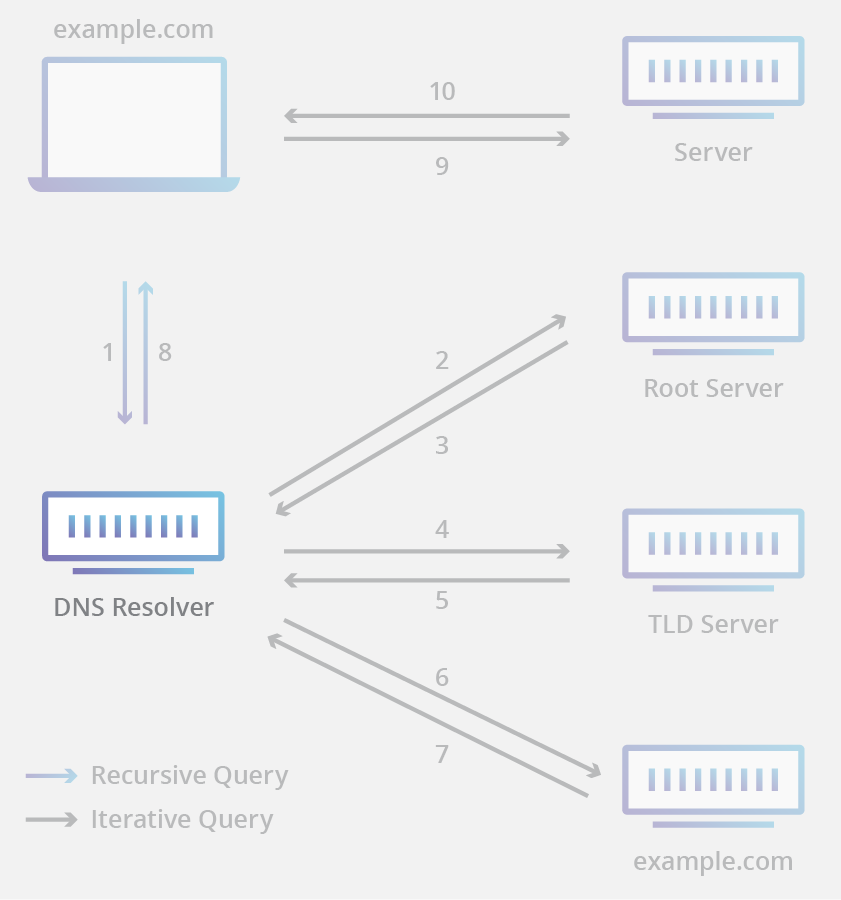
\includegraphics[width=\textwidth]{images/applications/recursive-resolver.png}
\caption{\acs{DNS} address resolution}
\label{fig:dns}
\end{figure}



\paragraph{\acs{mDNS}}
   \iacs{mDNS}
When a \acl{mDNS} client needs to resolve a hostname, it sends an \acs{IP} multicast query message that asks the host having that name to identify itself.
That target machine then multicasts a message that includes its \acs{IP} address.
All machines in that subnet can then use that information to update their \acs{mDNS} caches.
Any host can relinquish its claim to a name by sending a response packet with a \acf{TTL} equal to zero.
   \iacs{TTL}

By default, \acs{mDNS} exclusively resolves hostnames ending with the `.local' top-level domain.
This can cause problems if .local includes hosts that do not implement \acs{mDNS} but that can be found via a conventional unicast \acs{DNS} server.
Resolving such conflicts requires network configuration changes that \acs{mDNS} was designed to avoid.


\section{Email}
   \index{email}
Email operates across computer networks, primarily the Internet, and also local-area networks.
Today's email systems are based on a store-and-forward model.
Email servers accept, forward, deliver, and store messages.
Neither the users nor their computers are required to be online simultaneously; they need to connect, typically to a mail server or a webmail interface to send or receive messages or download it.


\paragraph{\acs{SMTP}}
   \iacs{SMTP}
The \acl{SMTP} is an internet standard communication protocol for electronic mail transmission.
Mail servers and other message transfer agents use \acs{SMTP} to send and receive mail messages.
User-level email clients typically use \acs{SMTP} only for sending messages to a mail server for relaying, and typically submit outgoing email to the mail server on port~587 or~465 per \rfc{8314}.

\acs{SMTP} servers commonly use the \acf{TCP} on port number~25 (for plaintext) and~587 (for encrypted communications).


\paragraph{\acs{POP3}}
   \iacs{POP3}
The \acl{POP3} provides access via an \acs{IP} network for a user client application to a mailbox (\emph{maildrop}) maintained on a mail server.
The protocol supports download and delete operations for messages.
\acs{POP3} clients connect, retrieve all messages, store them on the client computer, and finally delete them from the server.
This design of \acs{POP3} and its procedures was driven by the need of users having only temporary Internet connections, such as dial-up access, allowing these users to retrieve email when connected, and subsequently to view and manipulate the retrieved messages when offline.

A \acs{POP3} server listens on well-known port number~110 for service requests.
Encrypted communication for \acs{POP3} is either requested after protocol initiation, using the \SC{STLS} command, if supported, or by \acs{POP3S}, which connects to the server using \acs{TLS} or \acs{SSL} on well-known \acs{TCP} port number~995.


\paragraph{\acs{IMAP}}
   \iacs{IMAP}
The \acl{IMAP} was designed with the goal of permitting complete management of an email box by multiple email clients, therefore clients generally leave messages on the server until the user explicitly deletes them.
An \acs{IMAP} server typically listens on port number~143.
\acs{IMAP} over \acs{SSL}/\acs{TLS} (\acs{IMAPS}) is assigned the port number~993.

\paragraph{webmail}
   \index{webmail}
Companies no longer host their own email servers using Postfix or Microsoft Exchange.
Instead they use cloud solutions like Gmail or Office~365.

\paragraph{spam}
   \index{spam}
Email spam, or \acf{UBE}, refers to the sending of unwanted or irrelevant emails to a large number of recipients.
These emails are often commercial in nature, and are sent in an attempt to promote products or services.
Email spam has steadily grown since the early 1990s, and by 2014 was estimated to account for around ninety percent of total email traffic.

\epigraph{\emph{``Two years from now, spam will be solved.''}}{Bill Gates, World Economic Forum meeting\\ Davos, Switzerland, 2004}

\section{Further reading}
\textcite{nemeth} explains all applications and protocols covered in this chapter in more detail and provides the details of how to setup name servers and mail servers.
Some interesting reads are \rfc{1912} and \rfc{2822}.

\Chapter{Cisco Packet Tracer}
\label{chap:cisco-pt}

\mode<article>{
Cisco's Packet Tracer is a powerful network \emph{simulation} tool which assists in learning about computer networks and enables you to practice the commands required to configure a computer network using Cisco hardware.
In this chapter we will touch on the basics required to get up and running with this powerful training aid.
}

\mode<article>{
\nocite{*}
\printbibliography
}
\end{document}
